% %%%%%%%%%%%%%%%%%%%%%%%%%%%%%%%%%%%%%%%%%%%%%%%%%%%%%%%%%%%%%%%%%%%%%%
% Dummy Chapter:
% %%%%%%%%%%%%%%%%%%%%%%%%%%%%%%%%%%%%%%%%%%%%%%%%%%%%%%%%%%%%%%%%%%%%%%

% %%%%%%%%%%%%%%%%%%%%%%%%%%%%%%%%%%%%%%%%%%%%%%%%%%%%%%%%%%%%%%%%%%%%%%
% The Introduction:
% %%%%%%%%%%%%%%%%%%%%%%%%%%%%%%%%%%%%%%%%%%%%%%%%%%%%%%%%%%%%%%%%%%%%%%
\fancychapter{Applications}
\label{cap:applications}

\slshape

In this chapter, we benchmark and compare our code with other implementations by simulating the Hubbard model in \acs{1D} and on the \acs{2D} square lattice, for which results are well established from either an analytical or numerical perspective.
Then, we consider the honeycomb lattice with both periodic and nanoribbon boundary conditions.
Finally, we carry out original calculations, applying our code to a minimal model of \acs{TMD} nanoribbons.
We compare our \acs{QMC} results with those also obtained by us in the mean field approximation.
The latter is formulated allowing a site and orbital-dependent mean field, and the self-consistency relation is solved numerically.
We characterize the convergence issues arising in this iterative procedure.

\normalfont

\section{One-dimensional Chain}
\label{sec:1d-chain}

The analytical solution of the \acs{1D} Hubbard model at half filling indicates that the ground state is antiferromagnetic \cite{lieb_absence_1968}.
To build a physical picture of the Hubbard chain, start by considering the $\frac{U}{t} \gg 1$ limit. 
Then, the Hubbard model can be replaced by an effective atomic Heisenberg model defined in the Hilbert subspace with one electron per site, and antiferromagnetic (AF) order sets in.
In the Hubbard model, at zero temperature, it is found that upon decreasing $U$, the system is not only \acs{AF} for large $U$, but remains an \acs{AF} \emph{insulator} down to $U \rightarrow 0$, becoming a \emph{conductor} and losing \acs{AF} order only at $U = 0$.
Thus, for high enough $\beta = 1 / T$, we expect to see signs of \acs{AF} order for all $0 < U < \infty$.
Upon decreasing $\beta$, thermal fluctuations tend to completely destroy long range order.
Conversely, as $\beta$ is increased, we expect to see a divergence in $\chi$, corresponding to a phase transition to the antiferromagnetic ground state.
We identify it by measuring both the equal-time and time-displaced spin-spin correlation functions, $\left\langle S^z_i  S^z_j \right\rangle$ and $\left\langle S^z_i (\tau) S^z_j (0) \right\rangle$ with Monte Carlo.
Fourier transforming as per Eqs.(\ref{eq:S(q)},\ref{eq:chi(q)}), we obtain a peak at $q = \pi$ in the magnetic structure factor $S ( q ) $, and in the magnetic susceptibility $\chi (q)$.
Both peaks increase in magnitude as temperature is decreased, and in fact, within statistical uncertainty, the \say{staggered} susceptibility $\chi (\pi)$ appears to diverge very near $T_c = 0$.
Contrastingly, the $q = 0$ components of both the structure factor and the susceptibility go to zero as the temperature is decreased, indicating  no sign of ferromagnetic ordering in the ground state (see Fig.(\ref{fig:corr_FT})).
\begin{figure}[H]
\hspace{0.2cm}
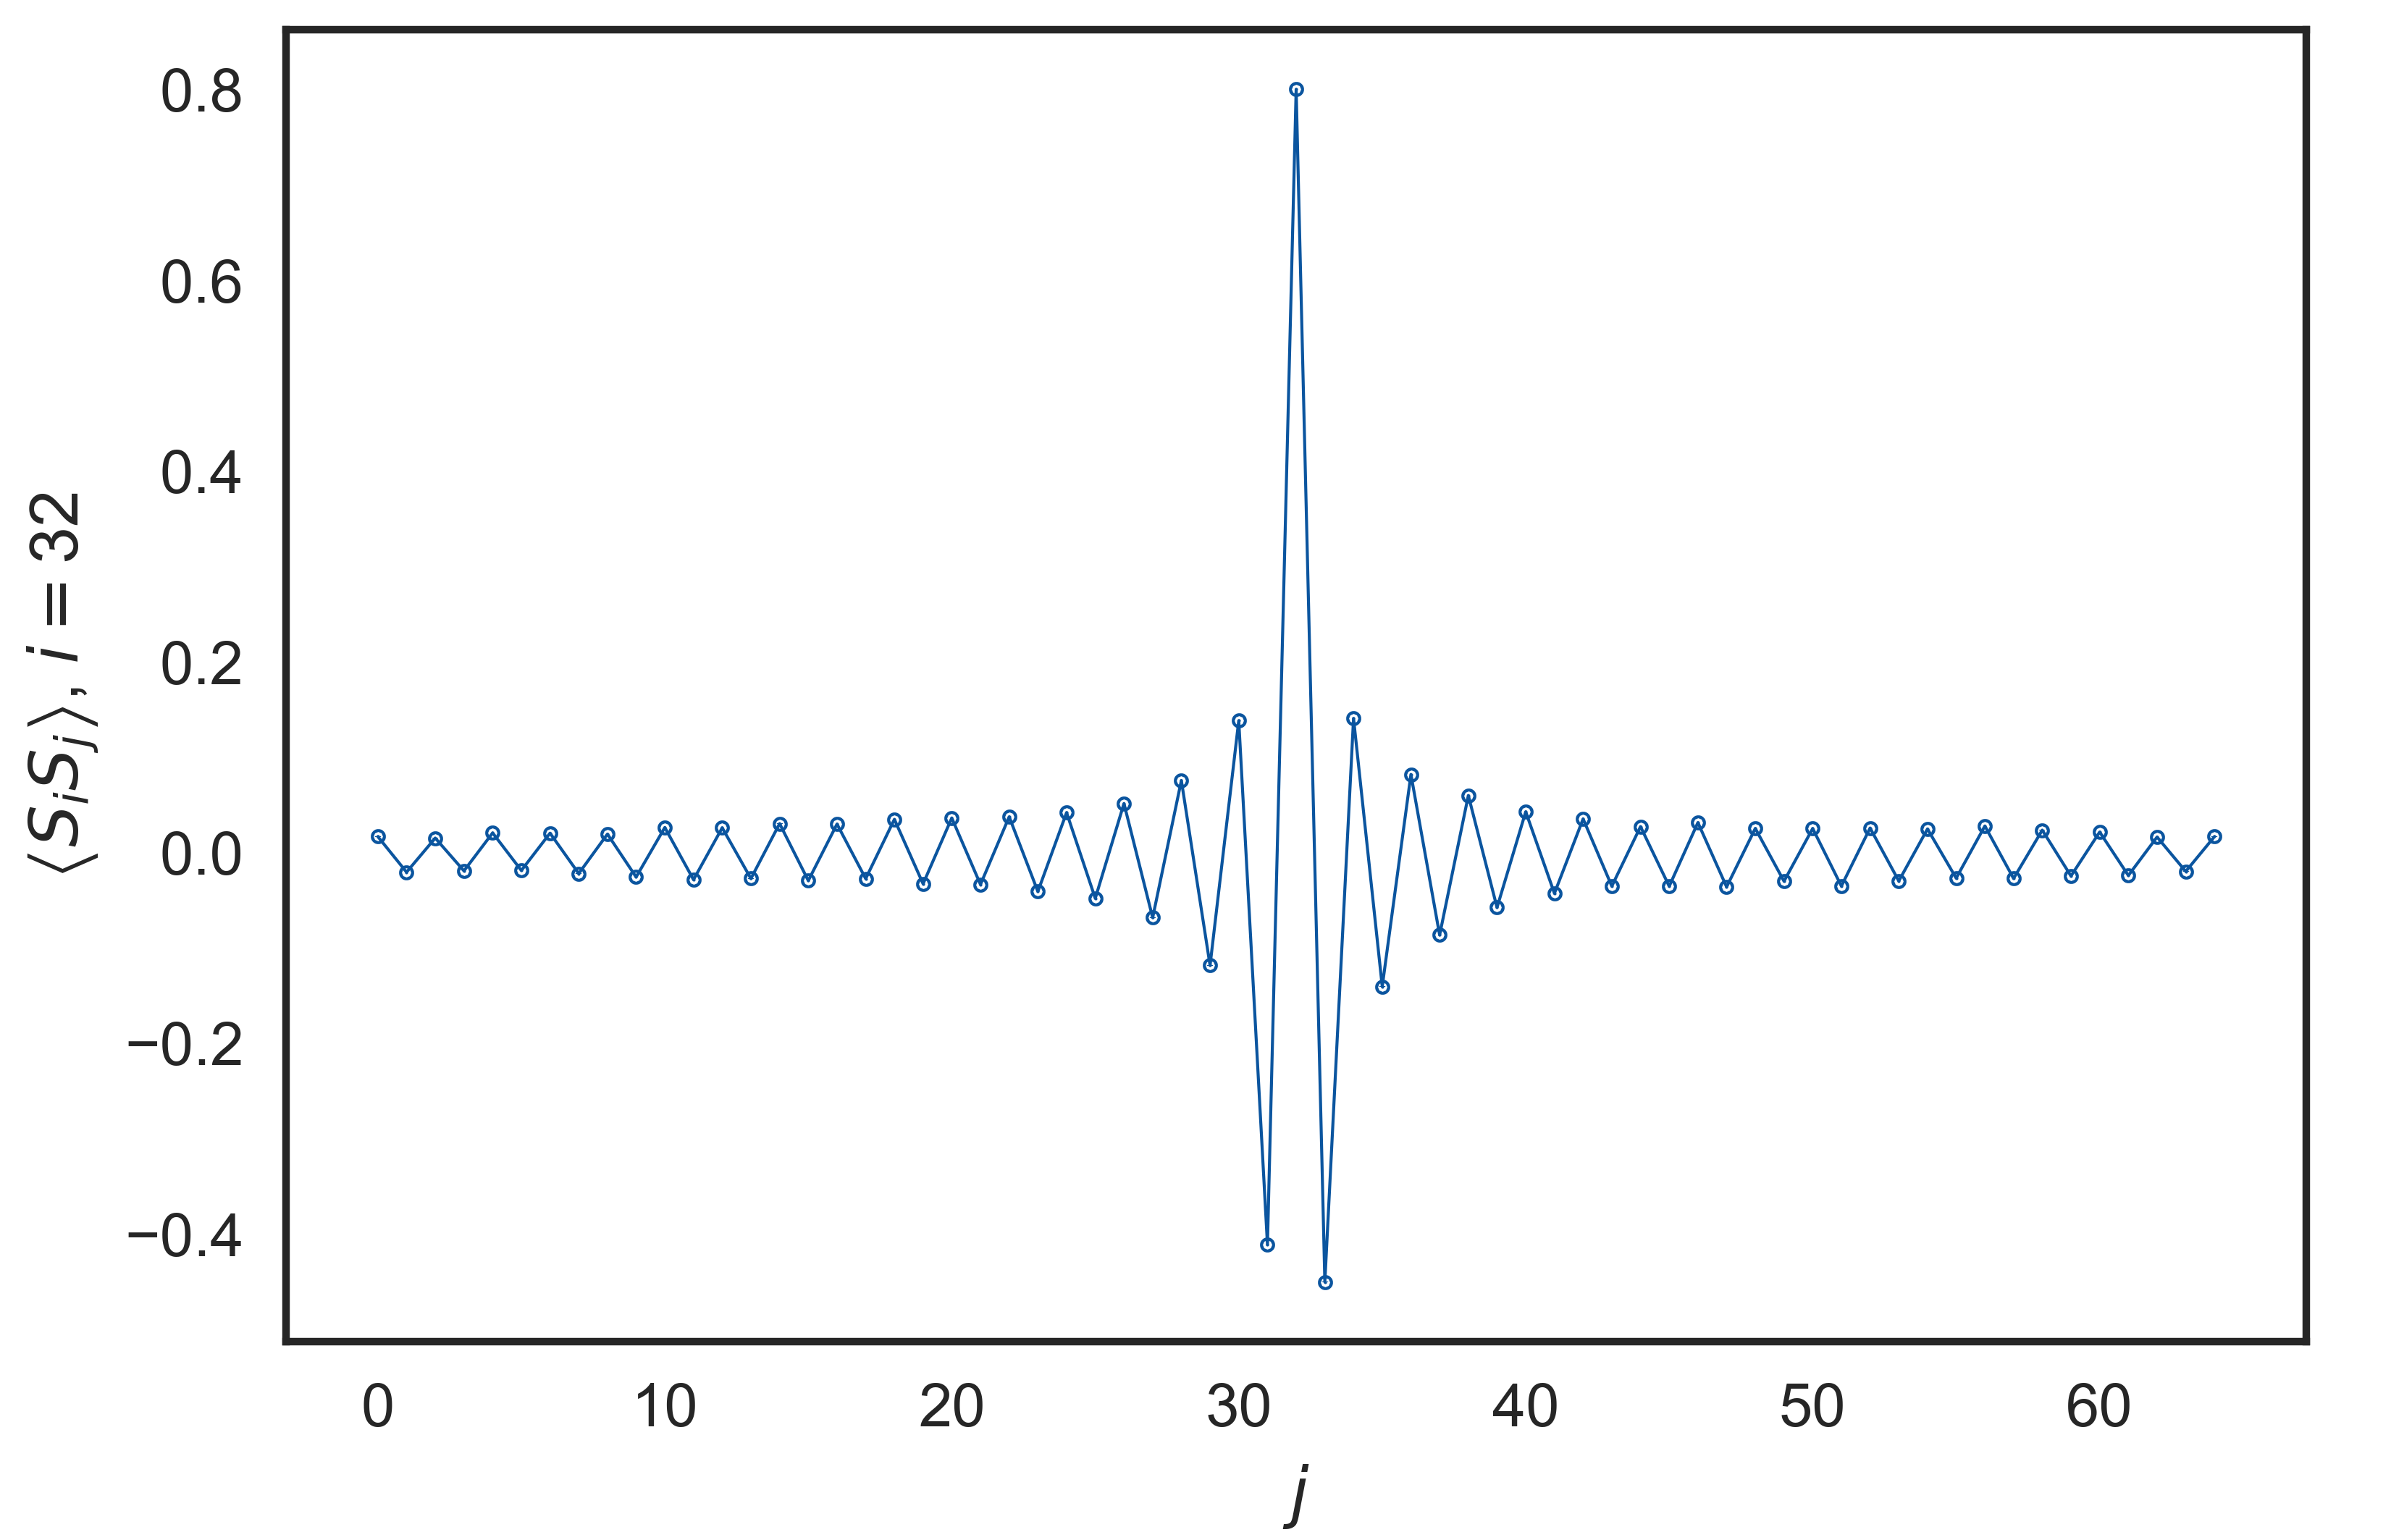
\includegraphics[scale=0.53]{Applications/magCorr.png}
\hspace{0.7cm}
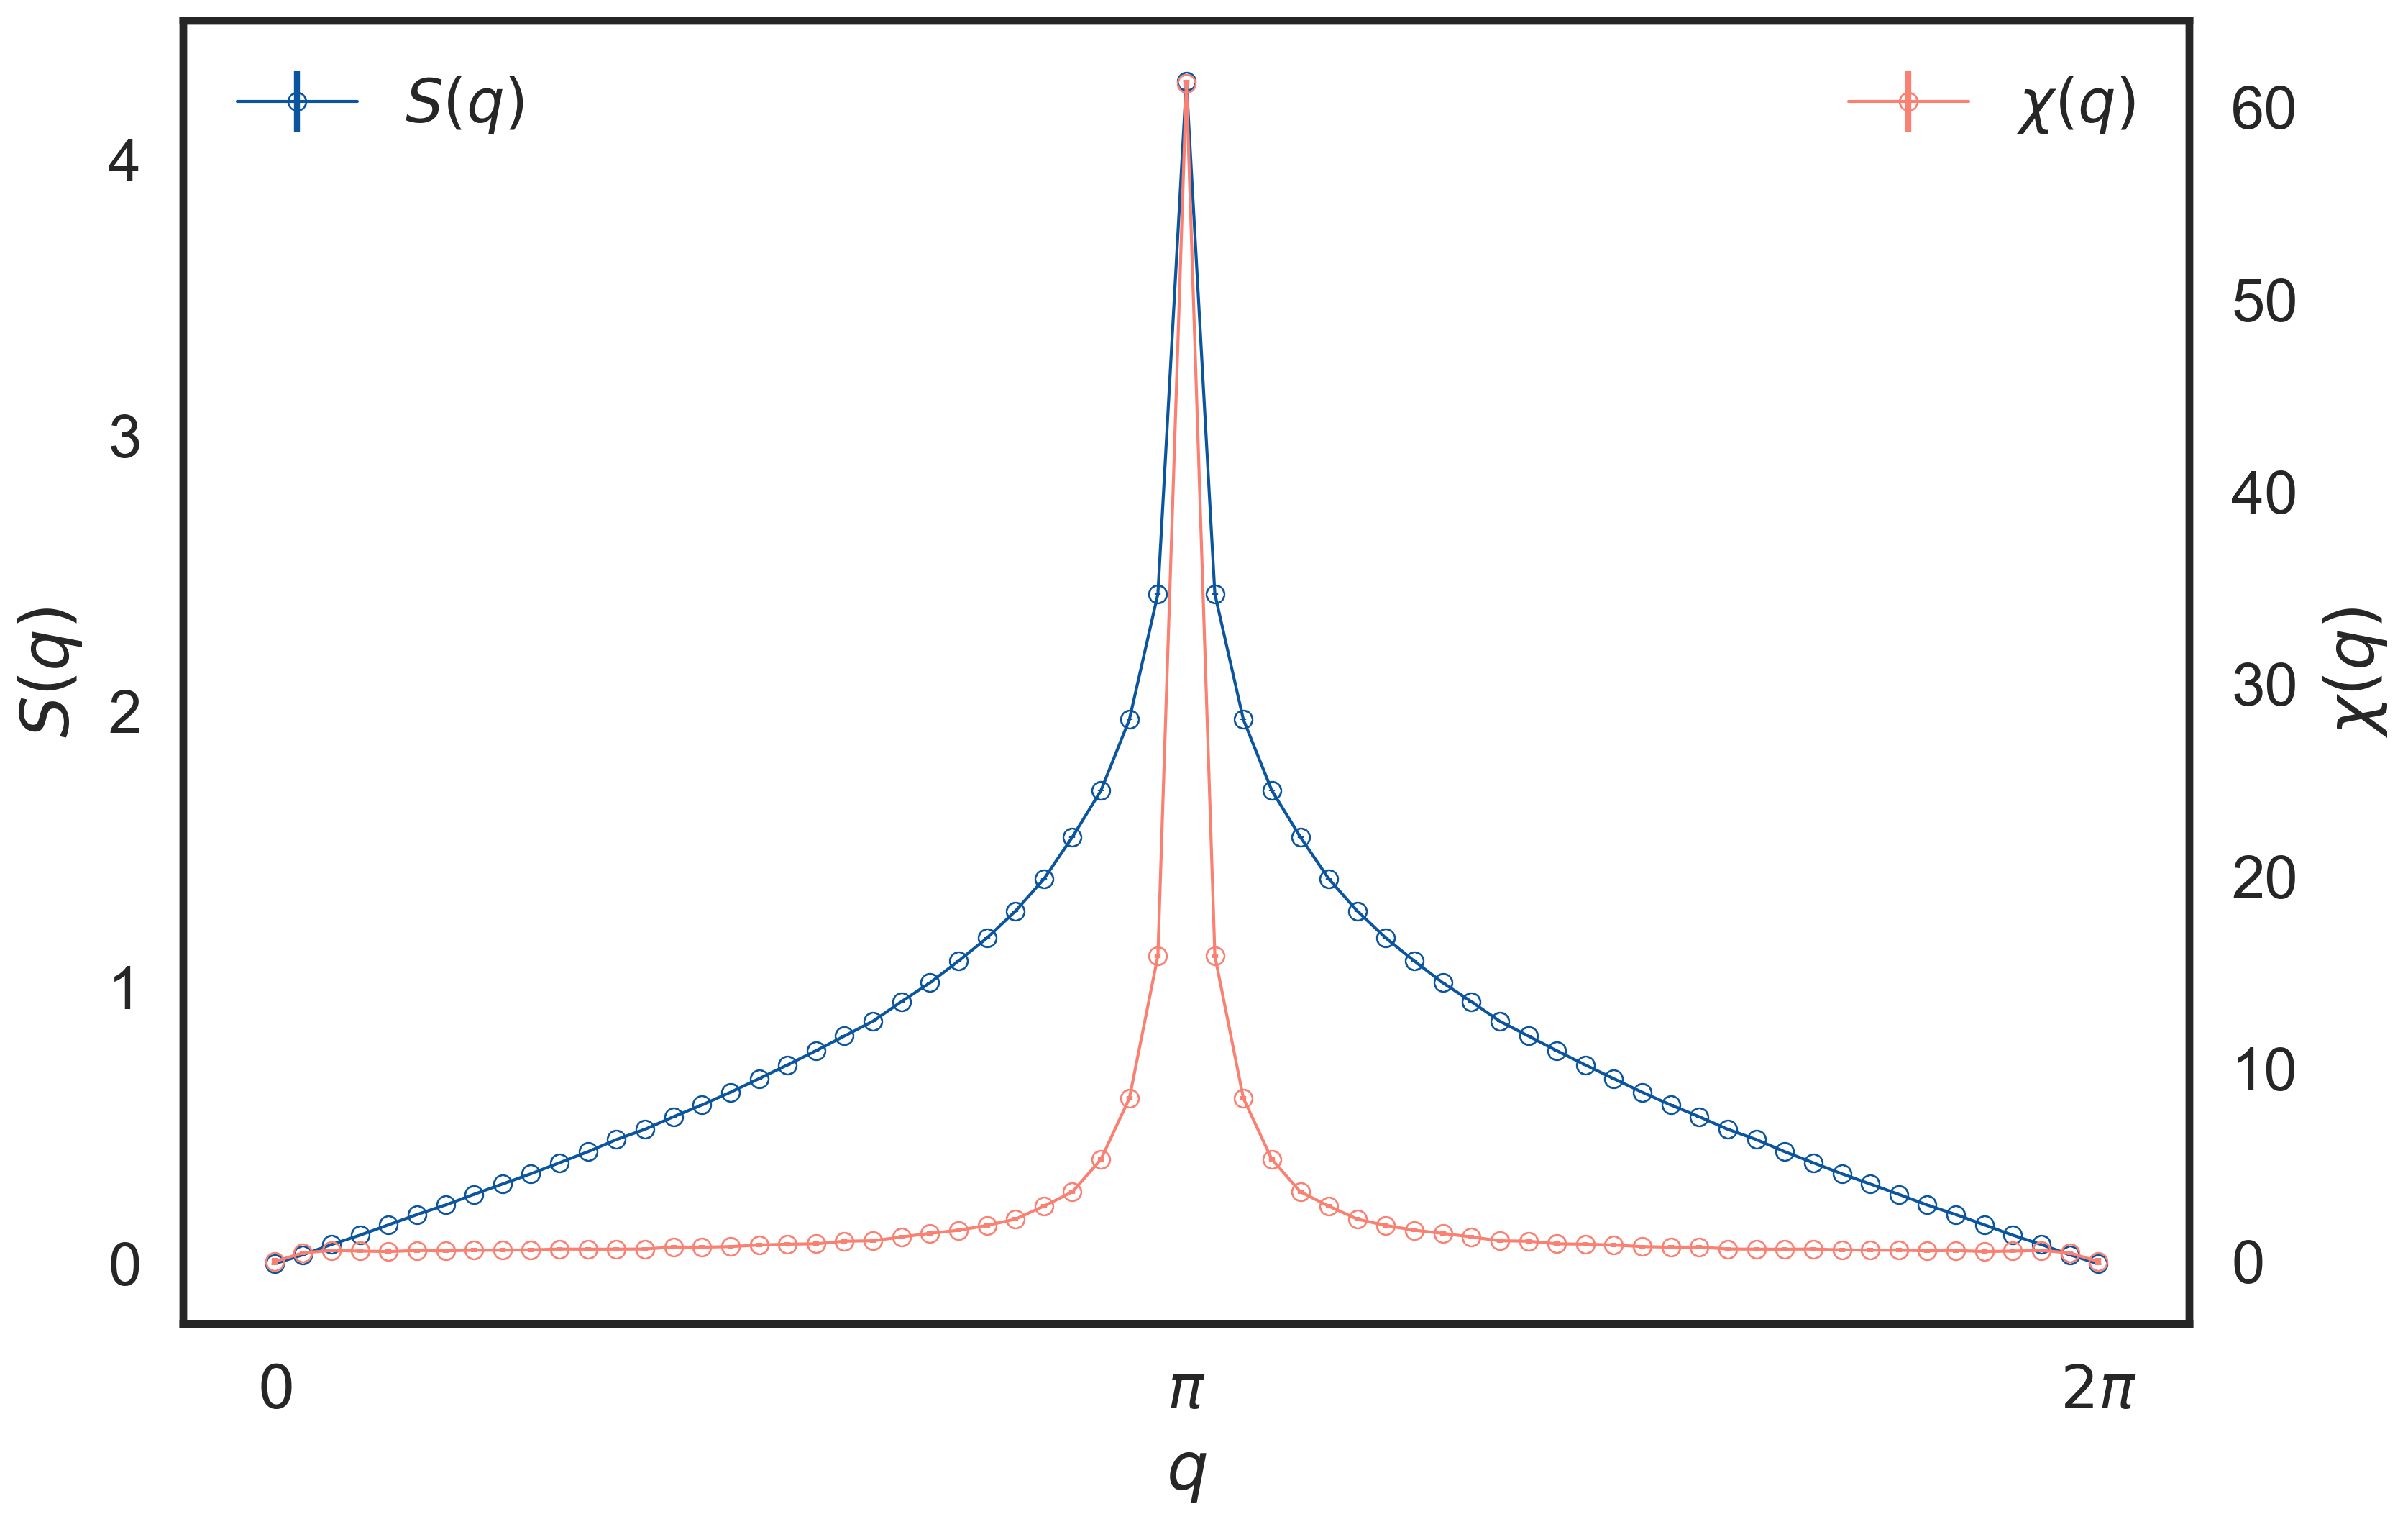
\includegraphics[scale=0.53]{Applications/SandChi.png}
\caption[Spin-spin correlation function, magnetic structure factor, and susceptibility for a 64 site Hubbard chain at $\beta t = 25 $, for $U = 4t$.]{Left: Spin-spin correlation function $\left\langle S^z_i S^z_j \right\rangle$ centered on the middle of the chain.
Right: Magnetic structure factor, and susceptibility for a 64-site Hubbard chain at $\beta t = 25 $, for $U = 4t$, at half filling $\left\langle n \right\rangle = 1$.\label{fig:corr_FT}}
\end{figure}
%According to spin-wave theory, the magnetic susceptiblity can be obtained from the spin-wave dispersion relation $\varepsilon ( k ) \propto k$, and at low temperature, we have
%\begin{equation}
%\chi \propto \int k dk \frac{e^{\beta k}}{(e^{\beta k} -1)^2} \propto T \ln T
%\end{equation}
%
%We find that within statistical uncertainty (which is bigger for $q=0$ for both the structure factor and the susceptibility), our results match this limit at low temperature already at $U = 4t$ (see Fig.(\ref{fig:Schi0})).
%\begin{figure}[H]
%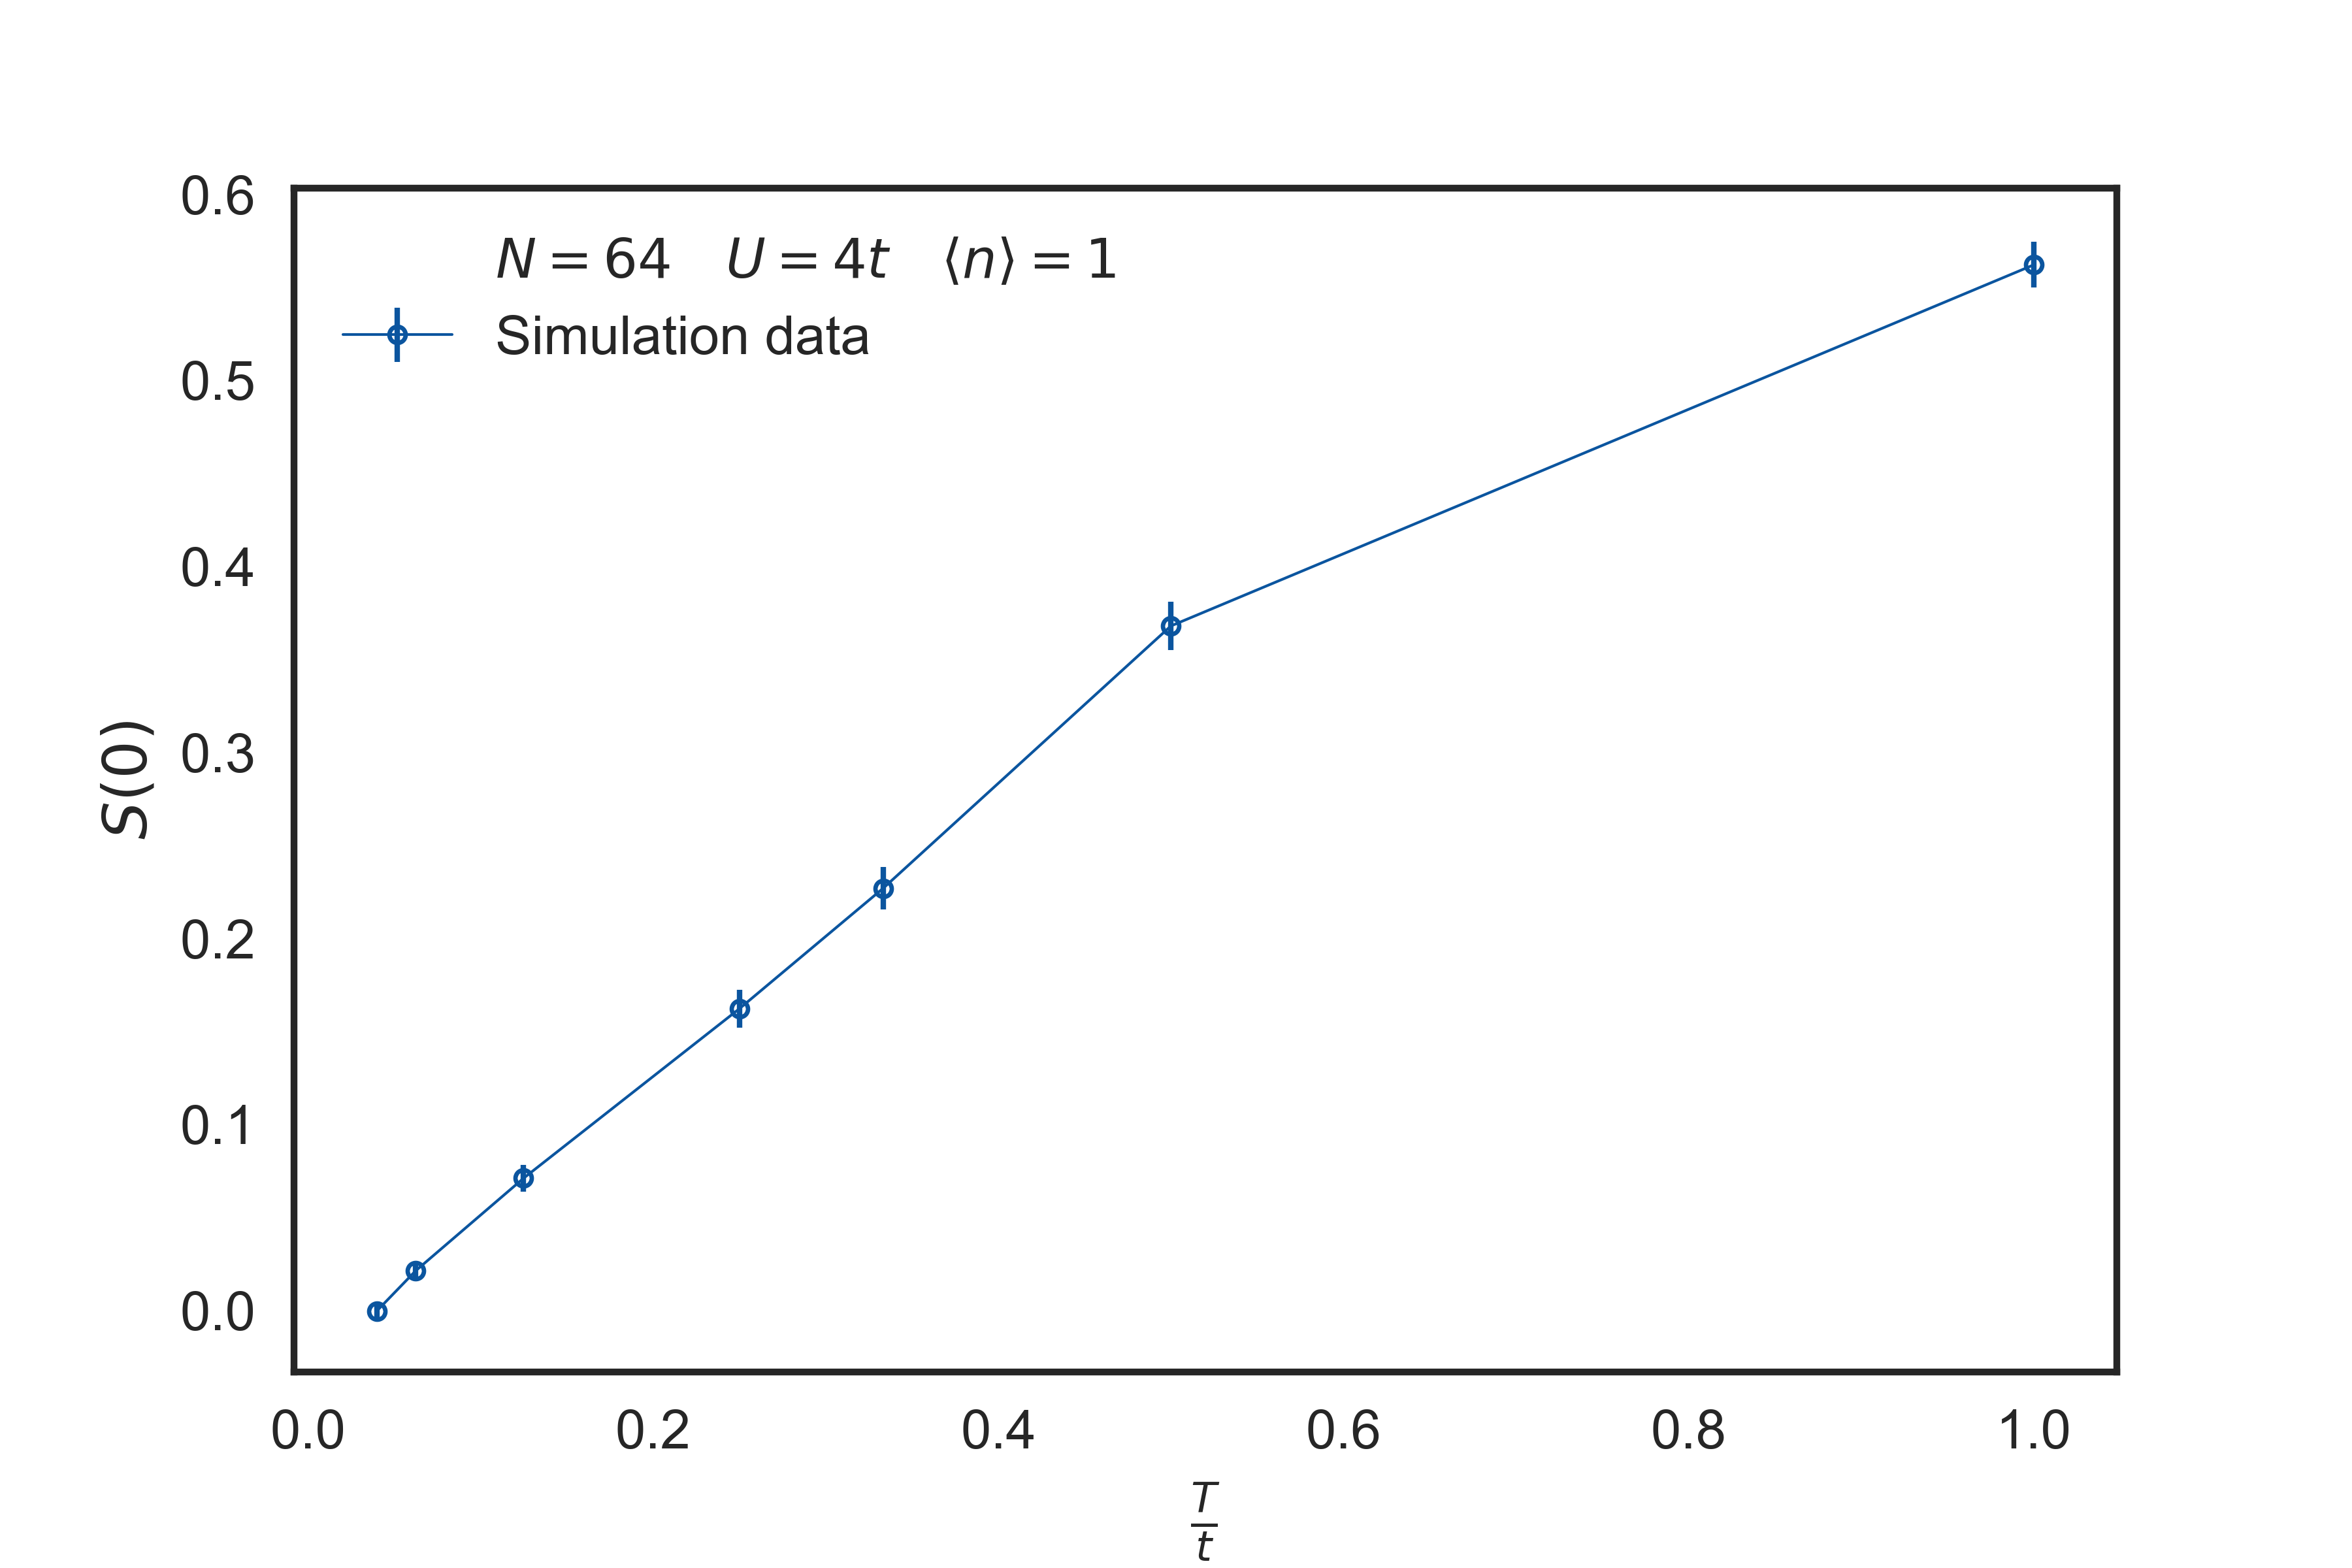
\includegraphics[scale=0.53]{Applications/S0T.png}
%\hspace{-0.5cm}
%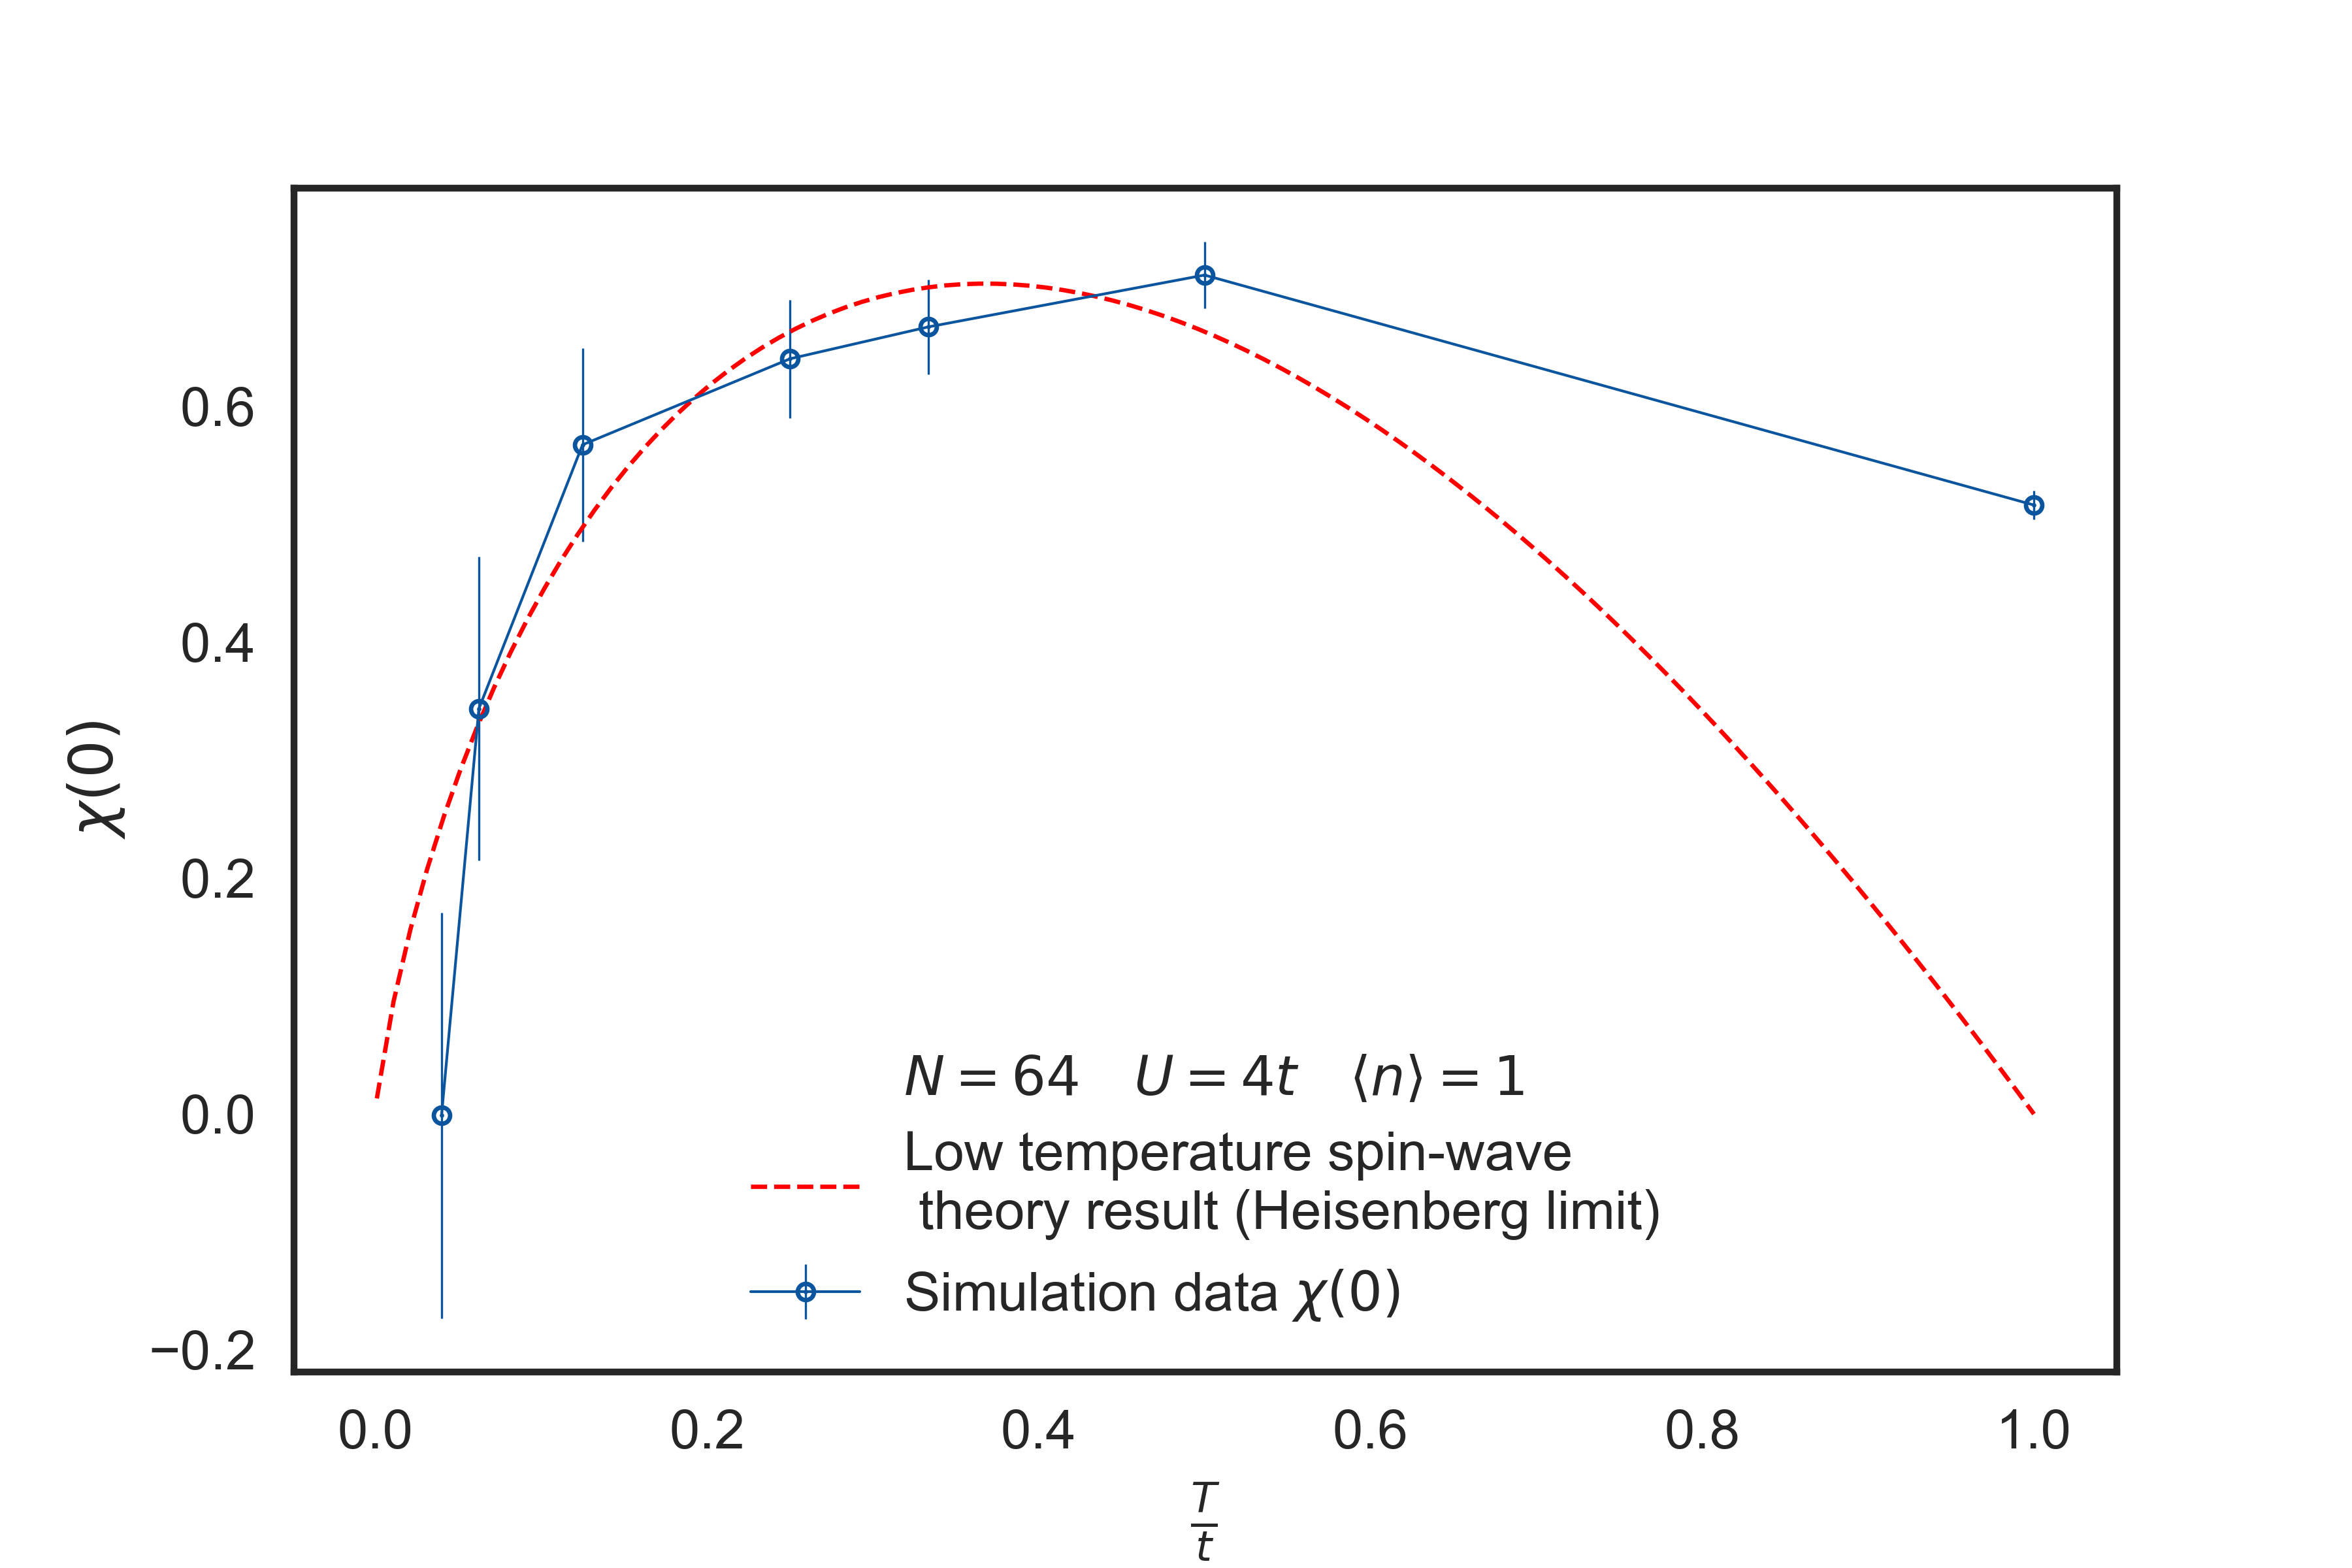
\includegraphics[scale=0.53]{Applications/Sus.png}
%\caption[$q=0$ components of the magnetic structure factor and susceptibility as a function of temperature, indicating that the ground state does not have ferromagnetic ordering.]{By performing simulations for varying temperature and looking at the $q=0$ components of the magnetic structure factor and susceptibility as a function of temperature, we see that the ground state does not have ferromagnetic ordering.
%Furthermore, our result agrees with the low temperature prediction of spin-wave theory for the Heisenberg model, the large $U$ limit of the Hubbard model.\label{fig:Schi0}}
%\end{figure}
In the Heisenberg limit, $U \gg t$, the staggered susceptibility $\chi_{\text{st}} \equiv \chi (\pi)$ diverges as $\chi_{\text{st}} ( T ) \propto 1 / (T - T_c) $.
Already at $U = 4 t$, we find exactly this behavior with a critical temperature $T_c$ very close to zero (see Fig.(\ref{fig:SchiPi})).
In fact, the ground state of the Hubbard model for the 1D chain is also antiferromagnetic, hence the divergence at $T_c = 0$ of the staggered susceptibility.
\vspace{-0.4cm}
\begin{figure}[H]
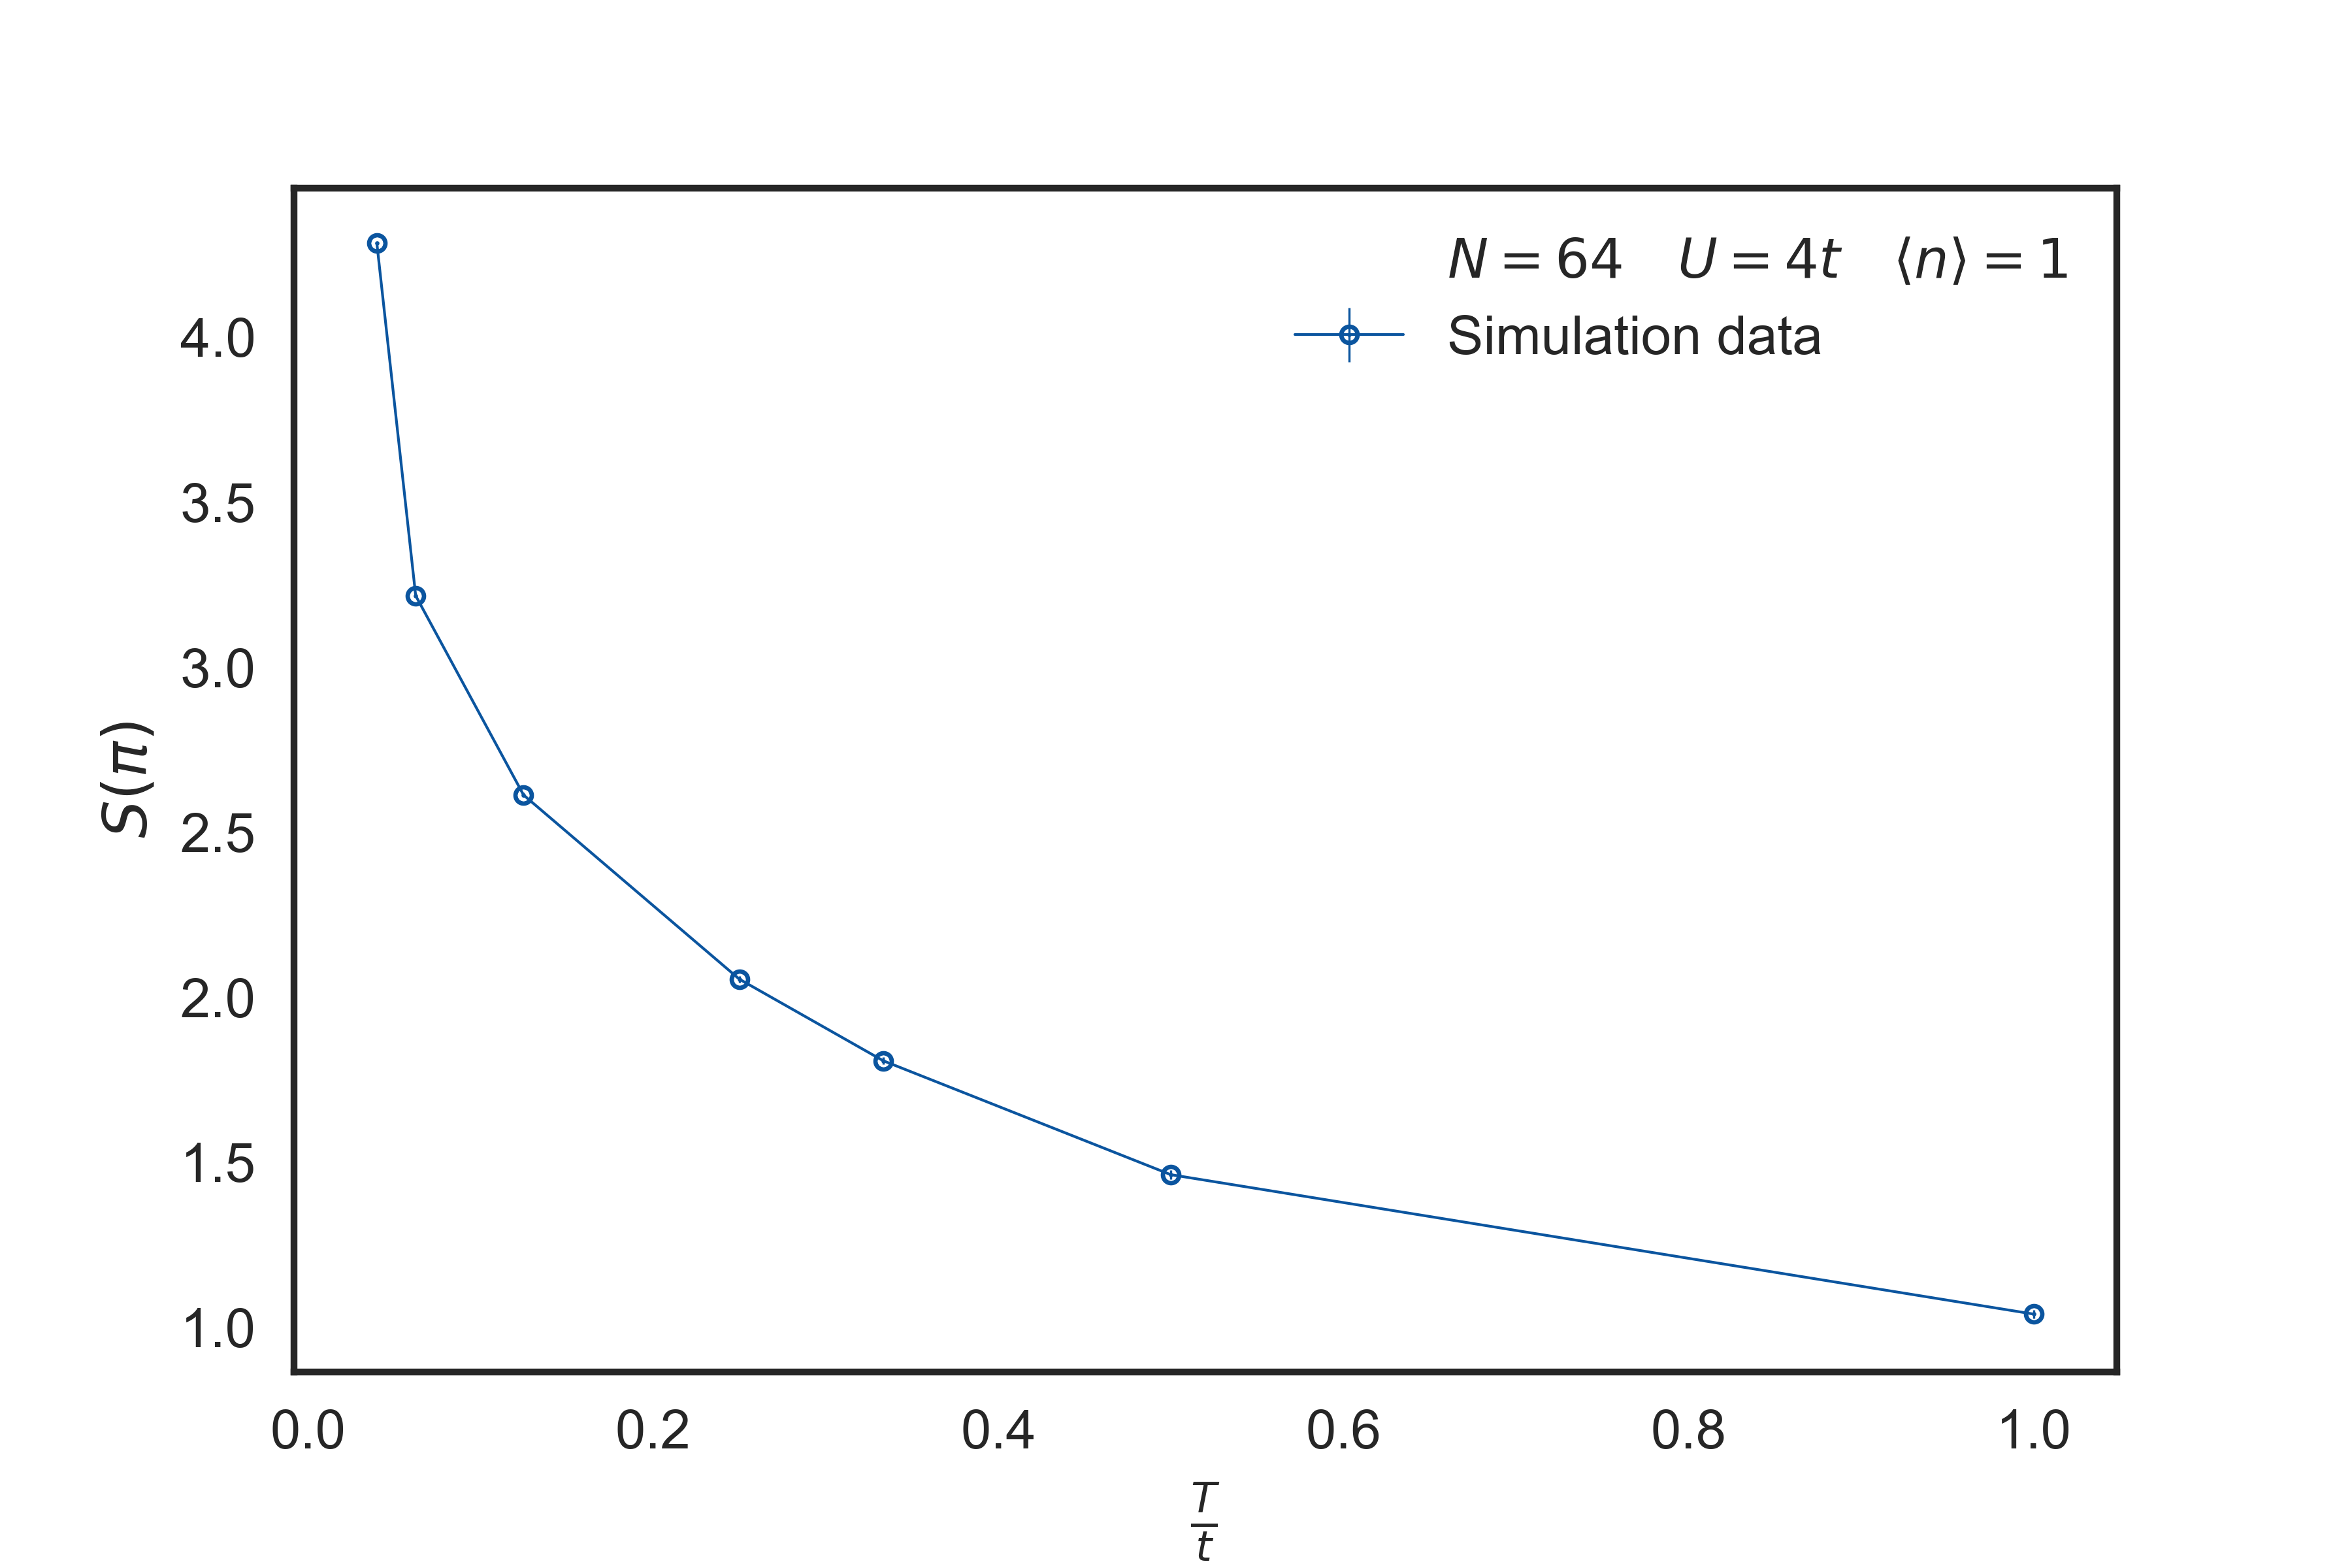
\includegraphics[scale=0.53]{Applications/SqT.png}
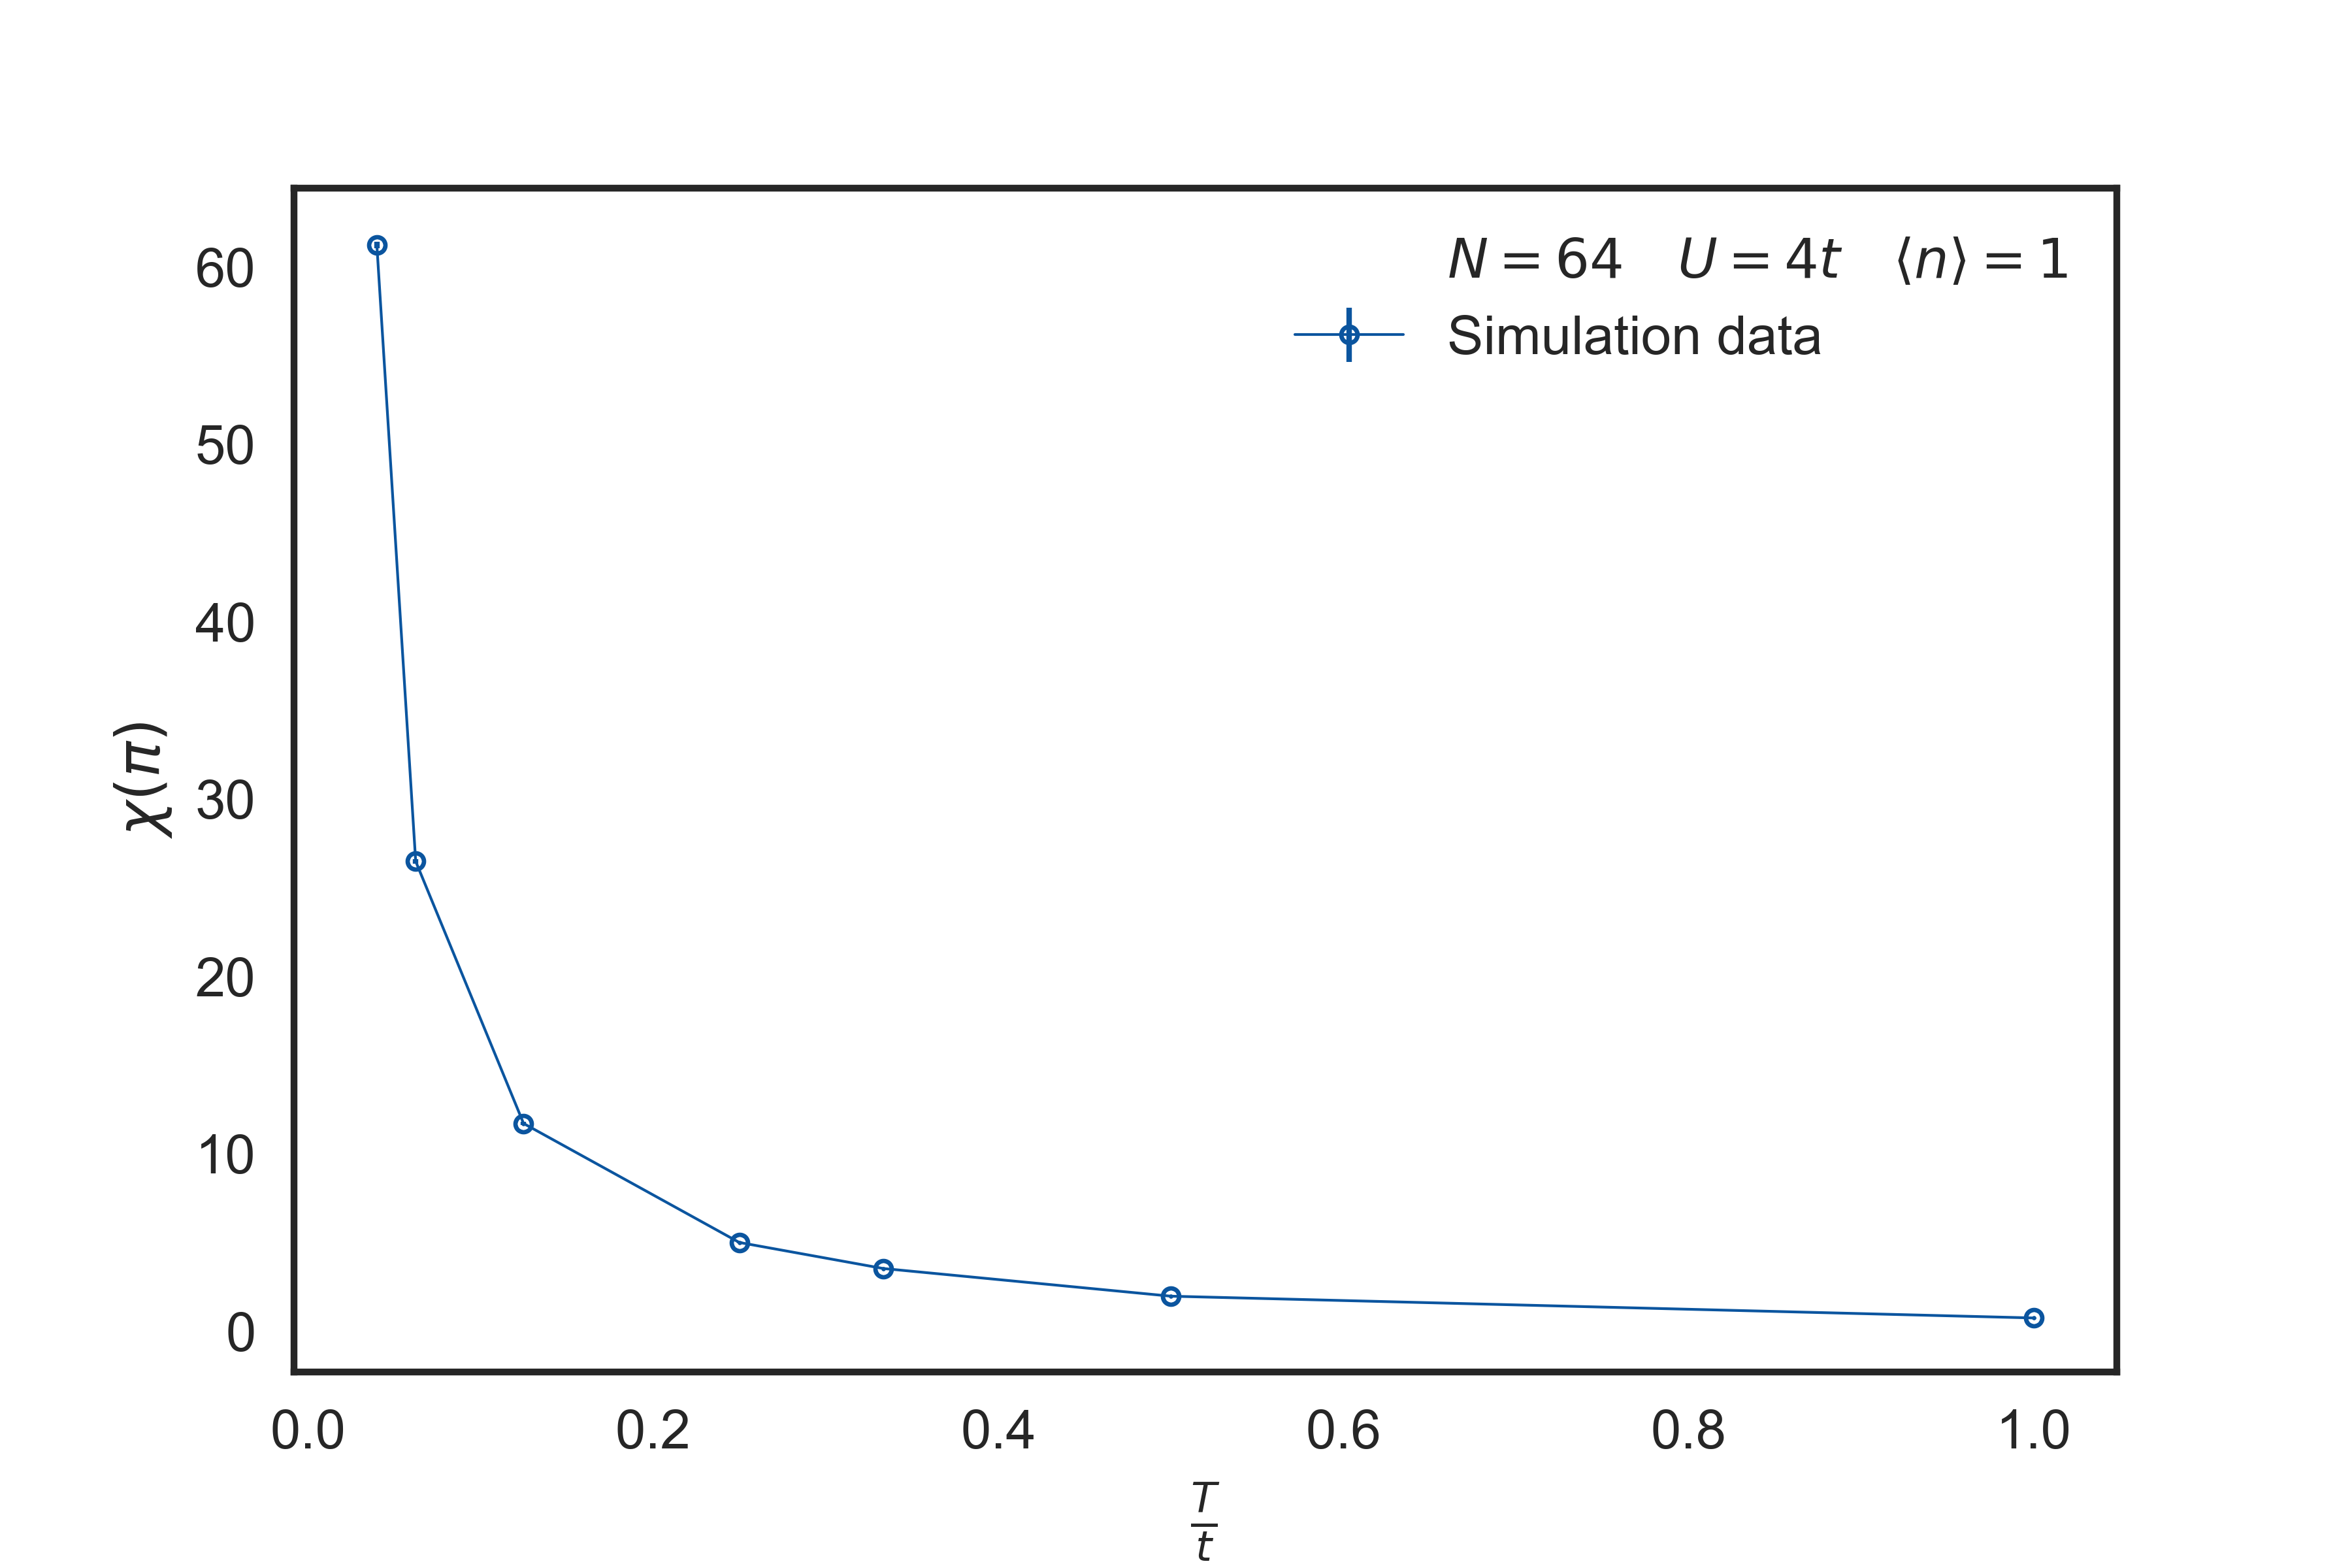
\includegraphics[scale=0.53]{Applications/stSus.png}
\caption[The magnetic structure factor and the  susceptibility have a peak at $q = \pi$ that increases as $T\rightarrow 0$, indicating \emph{antiferromagnetic ordering}.
 Divergence of the staggered susceptibility near $T_c = 0$, signaling the transition to the antiferromagnetic ground state.]{The magnetic structure factor and the susceptibility have a peak at $q = \pi$ that increases as $T\rightarrow 0$, indicating antiferromagnetic ordering.
The staggered susceptibility diverges near $T_c = 0$ (not exactly 0 because the system is finite), signaling the transition to the antiferromagnetic ground state.\label{fig:SchiPi}}
\end{figure}

We ran \texttt{QUEST} for the same 64-site chain we simulated with our code, using $\beta t = 25$, taking a half filled chain ($\left\langle n \right\rangle = 1$), and setting $U = 4t$.
We found a remarkable agreement between the measurements obtained using our code and using \texttt{QUEST}, namely in the magnetic structure factor, which we show in Fig.(\ref{fig:quest_time}).
Then, we took a small $2$-site system to compare the run time and verify the scaling with the number of slices ($\mathcal{O}(LN^3)$) of the determinant \ac{QMC} algorithm.
We noticed that \texttt{QUEST}'s algorithm suffers from large overhead time if the required precision via the Trotter error $\Delta \tau$, or the inverse temperature $\beta$ are large. 
This is due to the pre-conditioning needed to stabilize the products of the larger $L N \times L N$ matrices that are used in their algorithm (ours uses $N \times N$).
For large system sizes, \texttt{QUEST} is better than our algorithm because their implementation uses \emph{hybrid} \ac{QMC}, which (potentially) has subcubic $\mathcal{O}(LN)$ scaling (the cost of stabilizing the matrix product required to obtain the Green's matrix with sufficient accuracy at low temperature still scales with $N$ as $\mathcal{O}(N^3)$).

The results for the $2$-site system can be compared with the results obtained using exact diagonalization, a method which can only be used for small lattice sizes, and which we outlined in chapter \ref{cap:hubbard}.
We kept all the parameters, changing only the system size, and verified that our results agree with a similar study carried out in \cite{hirsch_discrete_1983}, confirming the validity of our implementation (see Fig.(\ref{fig:hirsch1982})).

\begin{figure}[H]
\hspace{0.1cm}
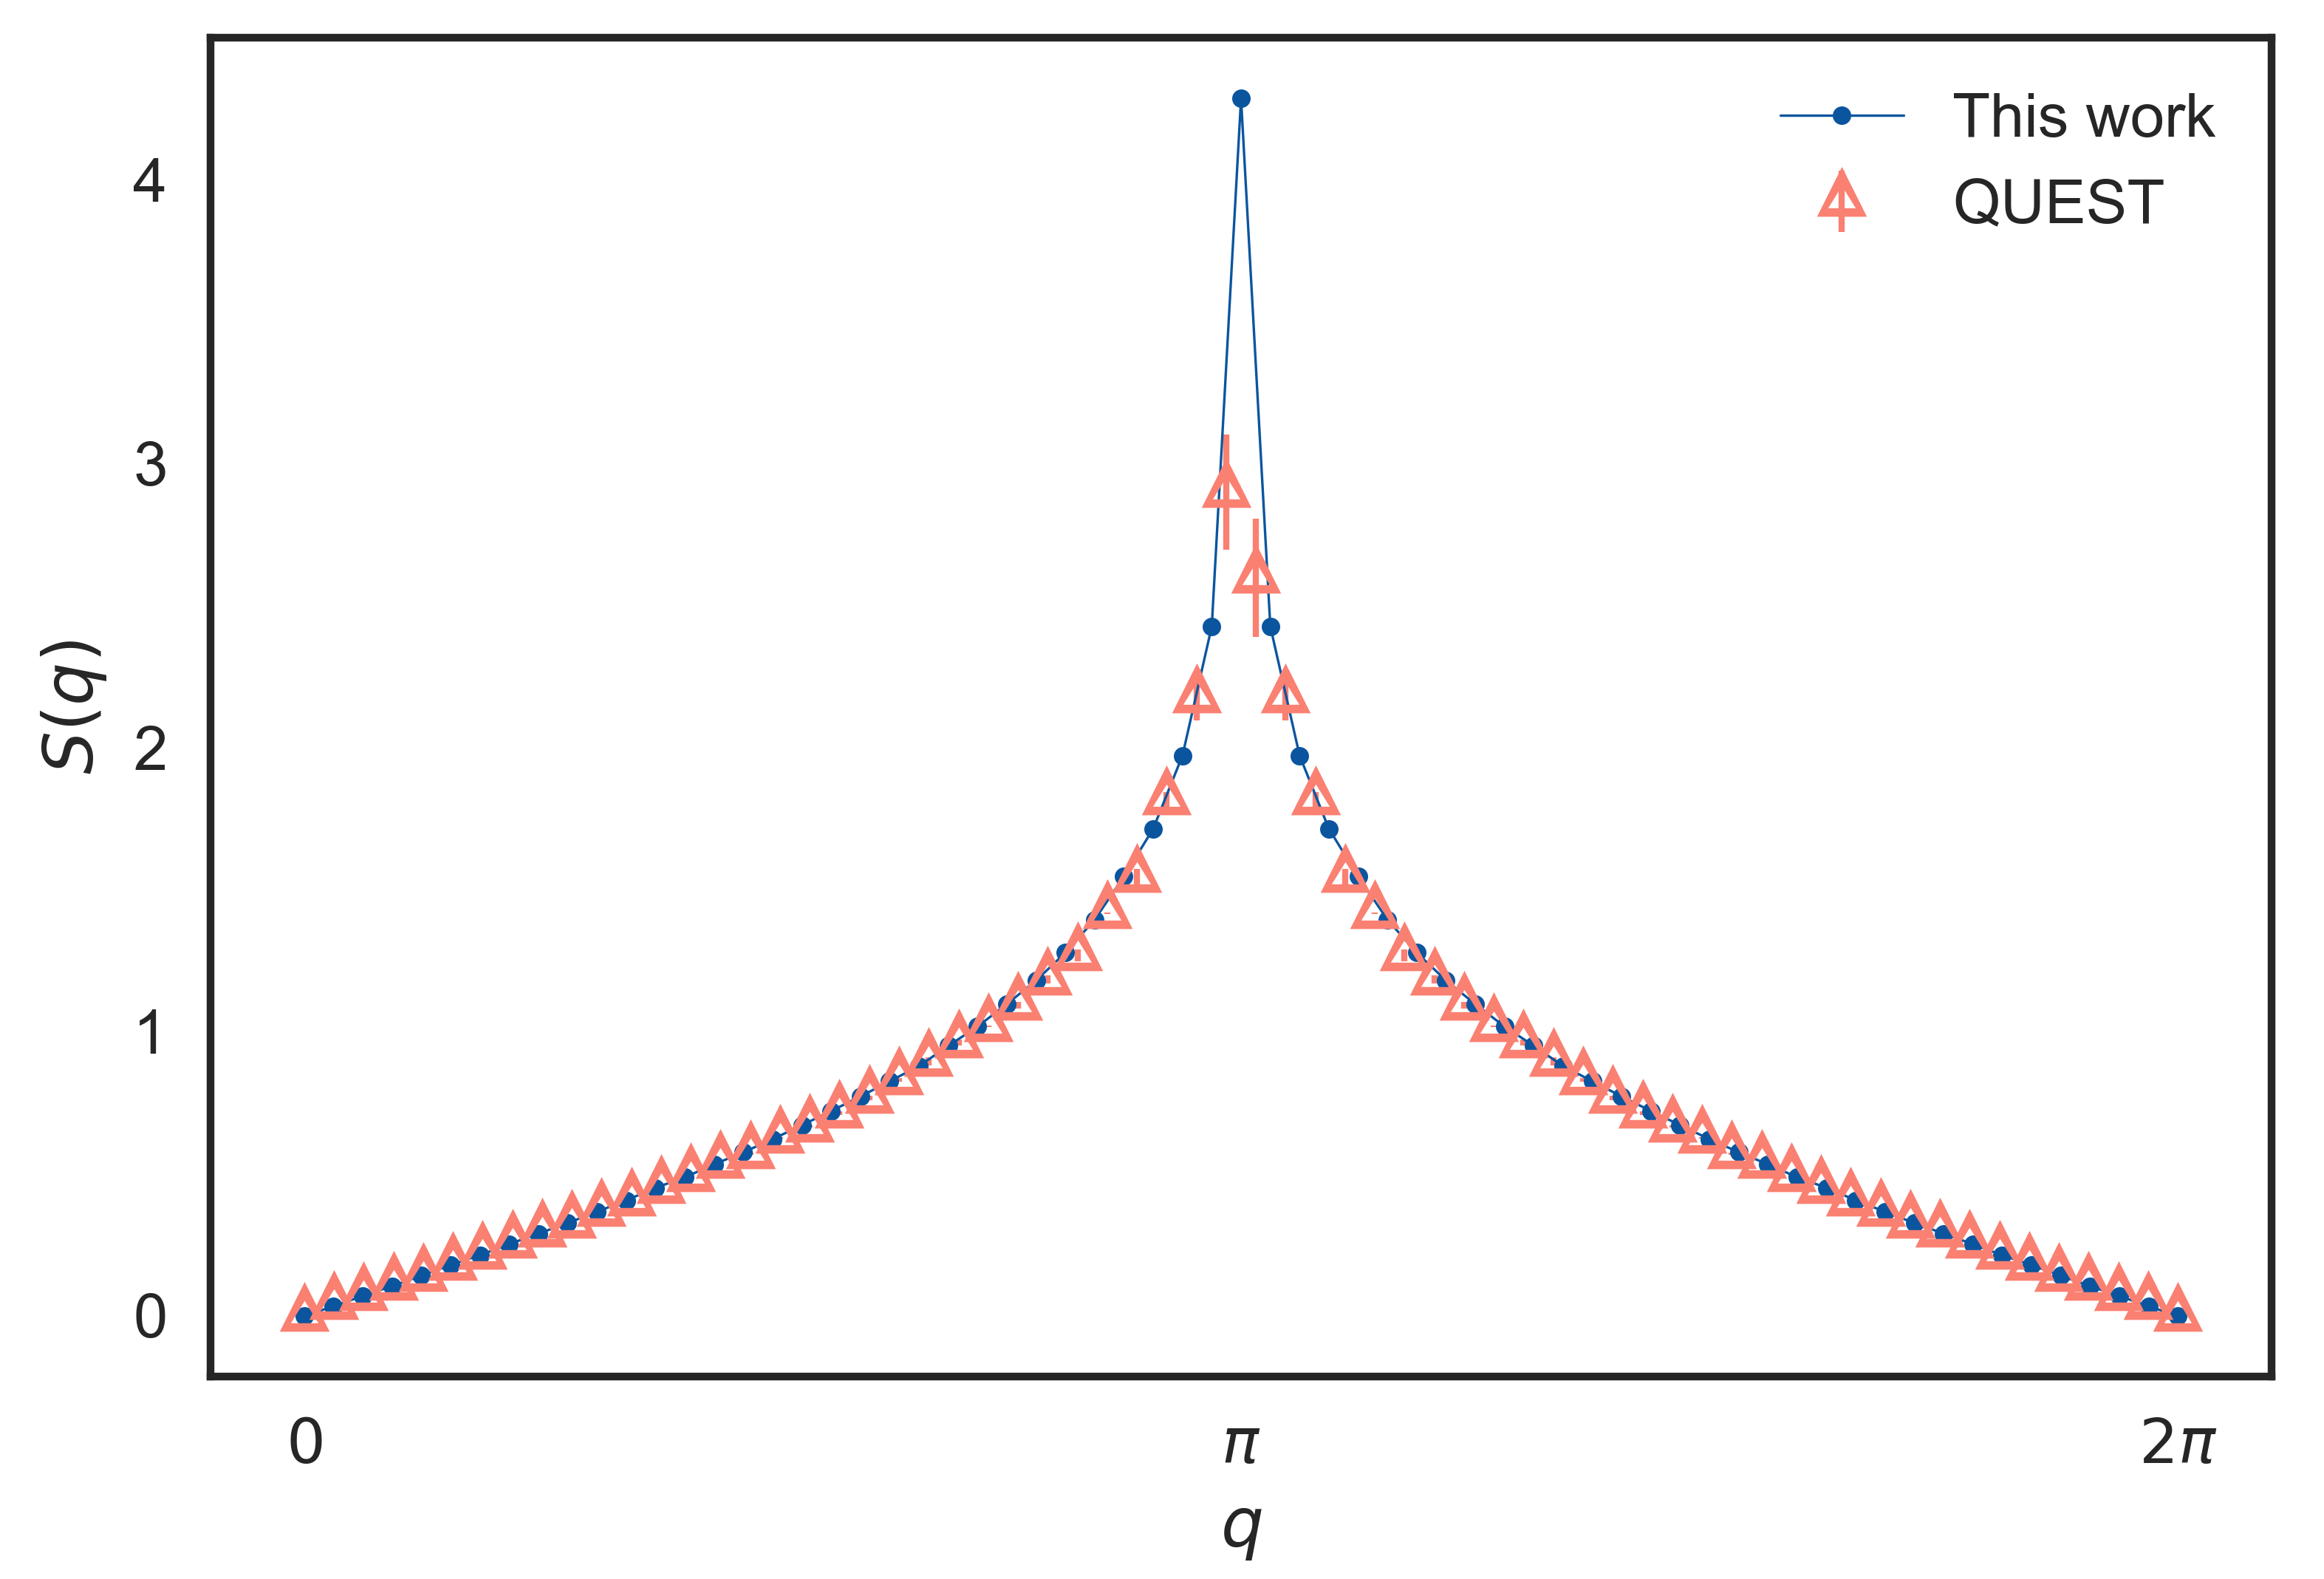
\includegraphics[scale=0.53]{Applications/s_compare.png}
\hspace{0.5cm}
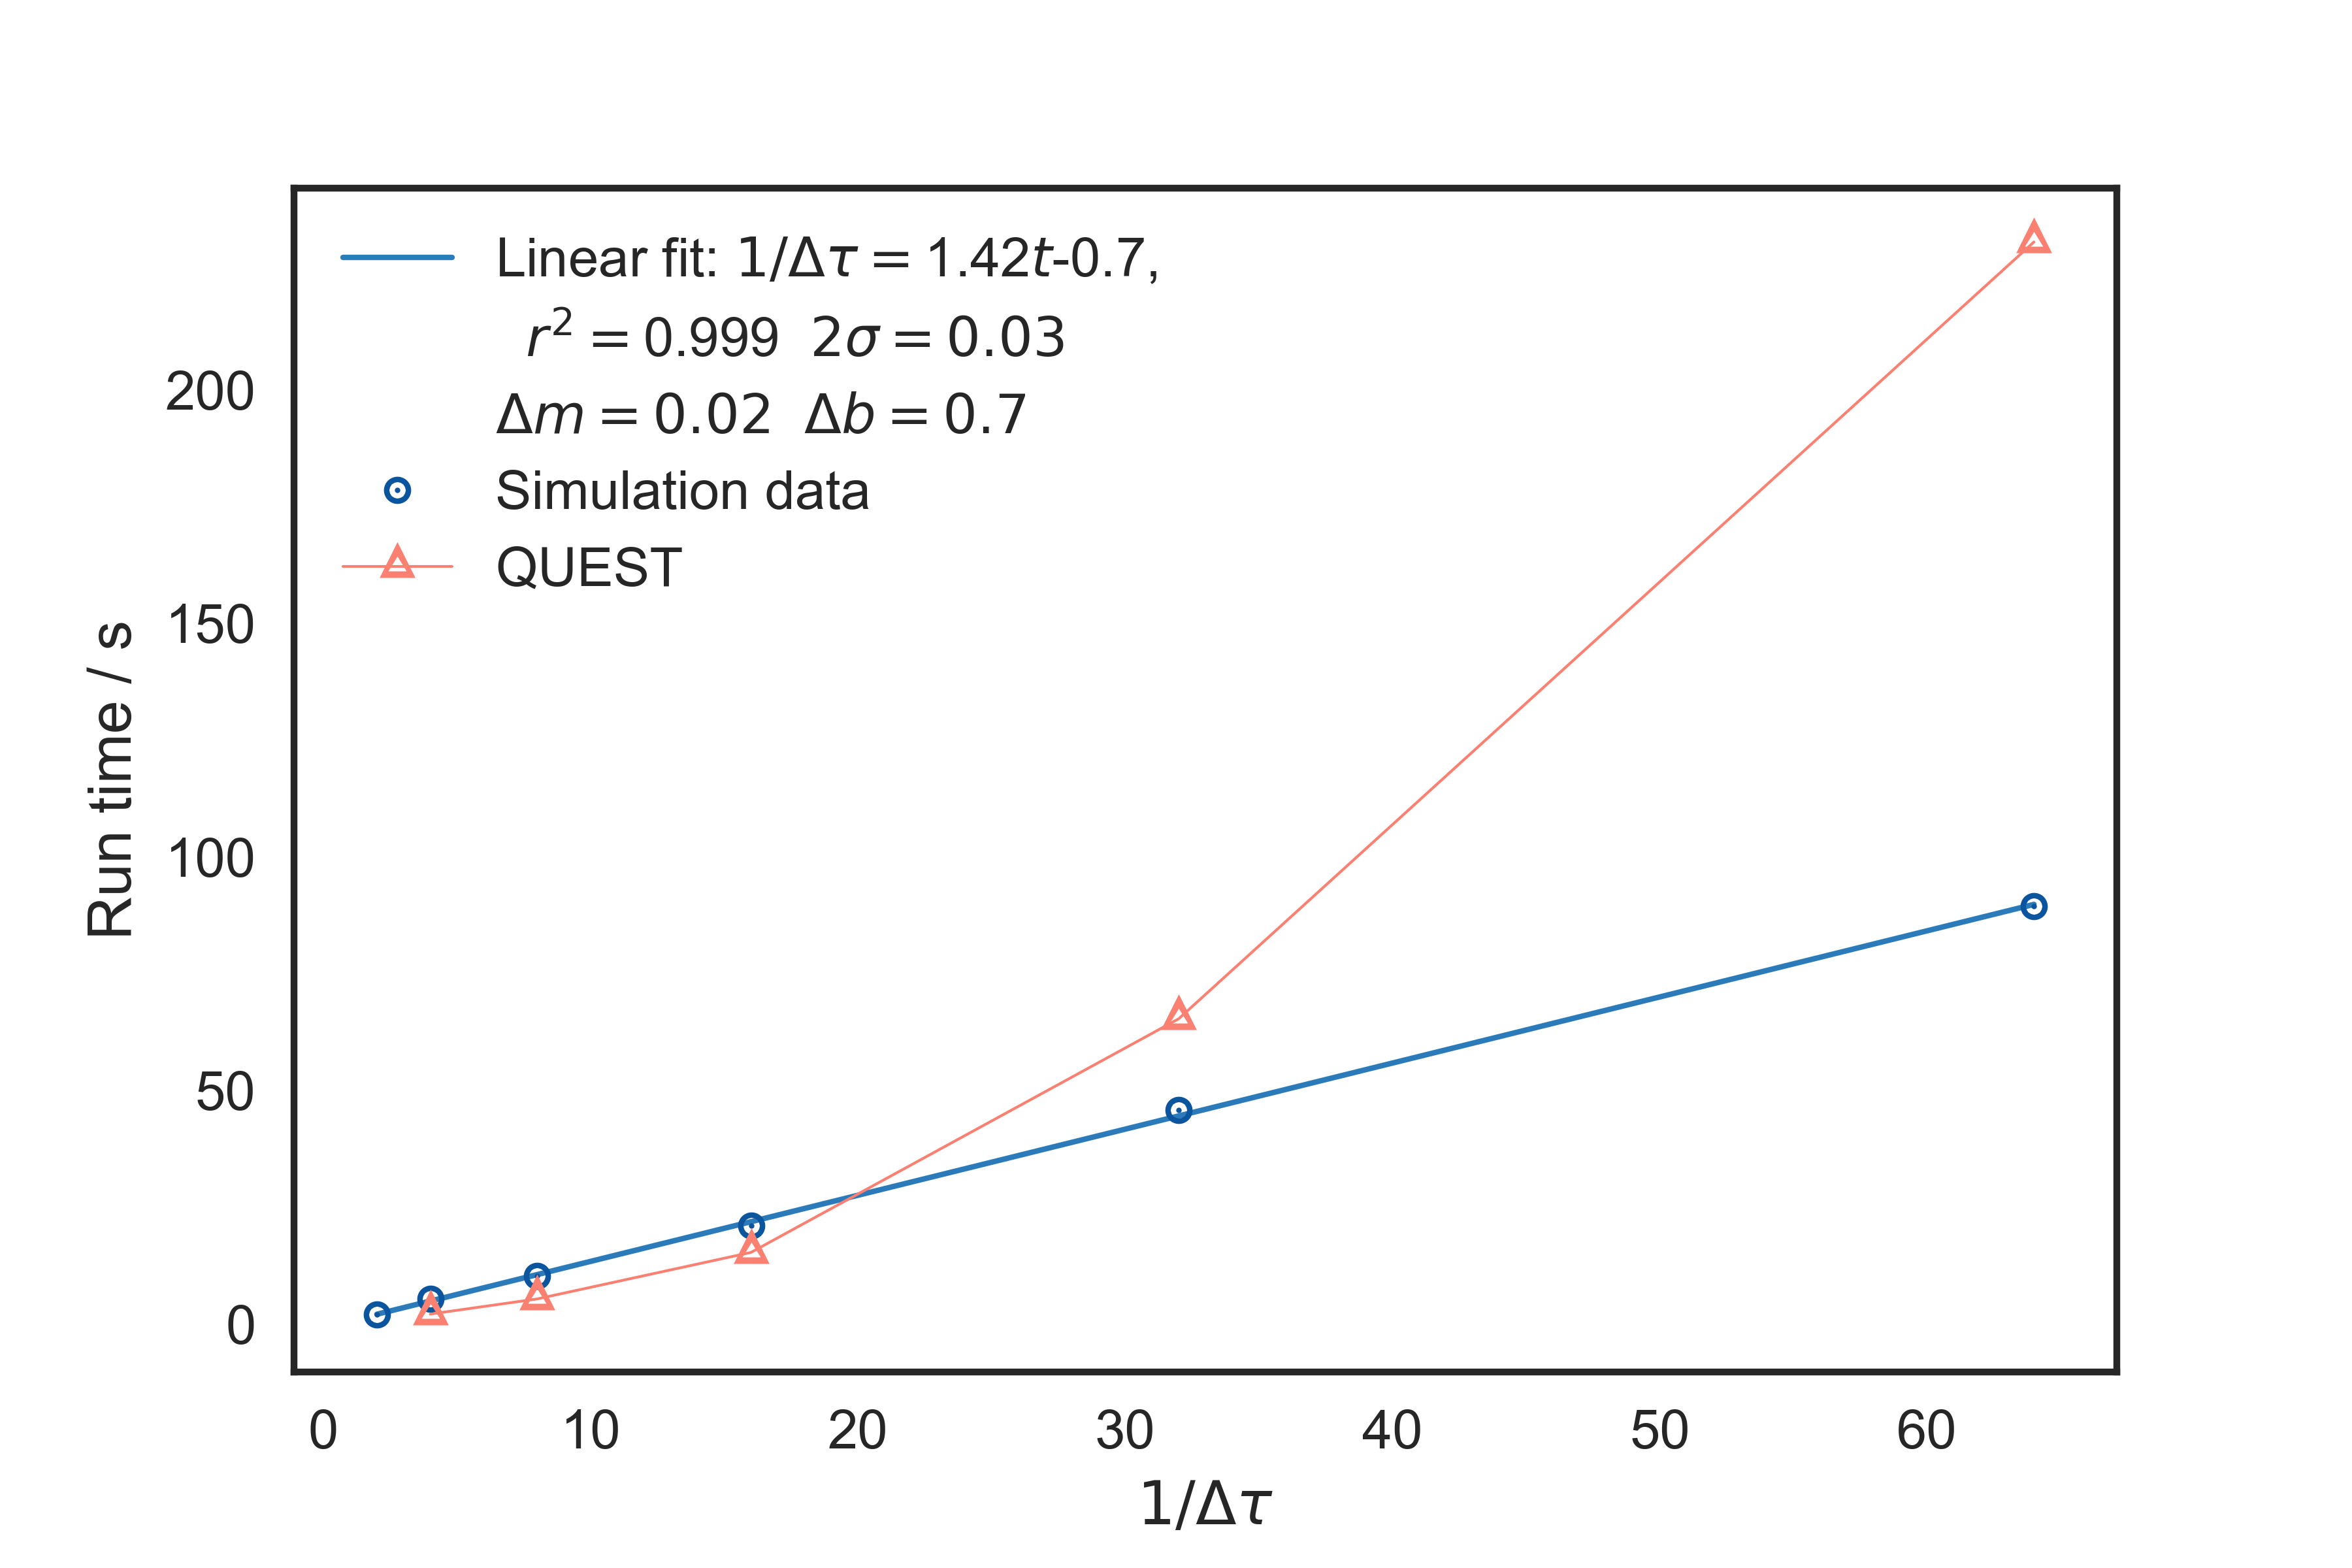
\includegraphics[scale=0.53]{Applications/runtime2sites.png}
\caption[Comparison of the magnetic structure factor with that obtained using \texttt{QUEST}. Run time comparison.]{Left: Comparison of the magnetic structure factor with that obtained using \texttt{QUEST}.
The used parameters are mentioned in the body of the text.
Right: The run time using our code increases linearly with $L$, as expected.
The \texttt{QUEST} algorithm initially scales linearly, but then becomes much slower due to the large overhead time associated with pre-conditioning the comparably much larger matrices they use if $L$ is very big.\label{fig:quest_time}}
\end{figure}
\vspace{-0.5cm}
\begin{figure}[H]
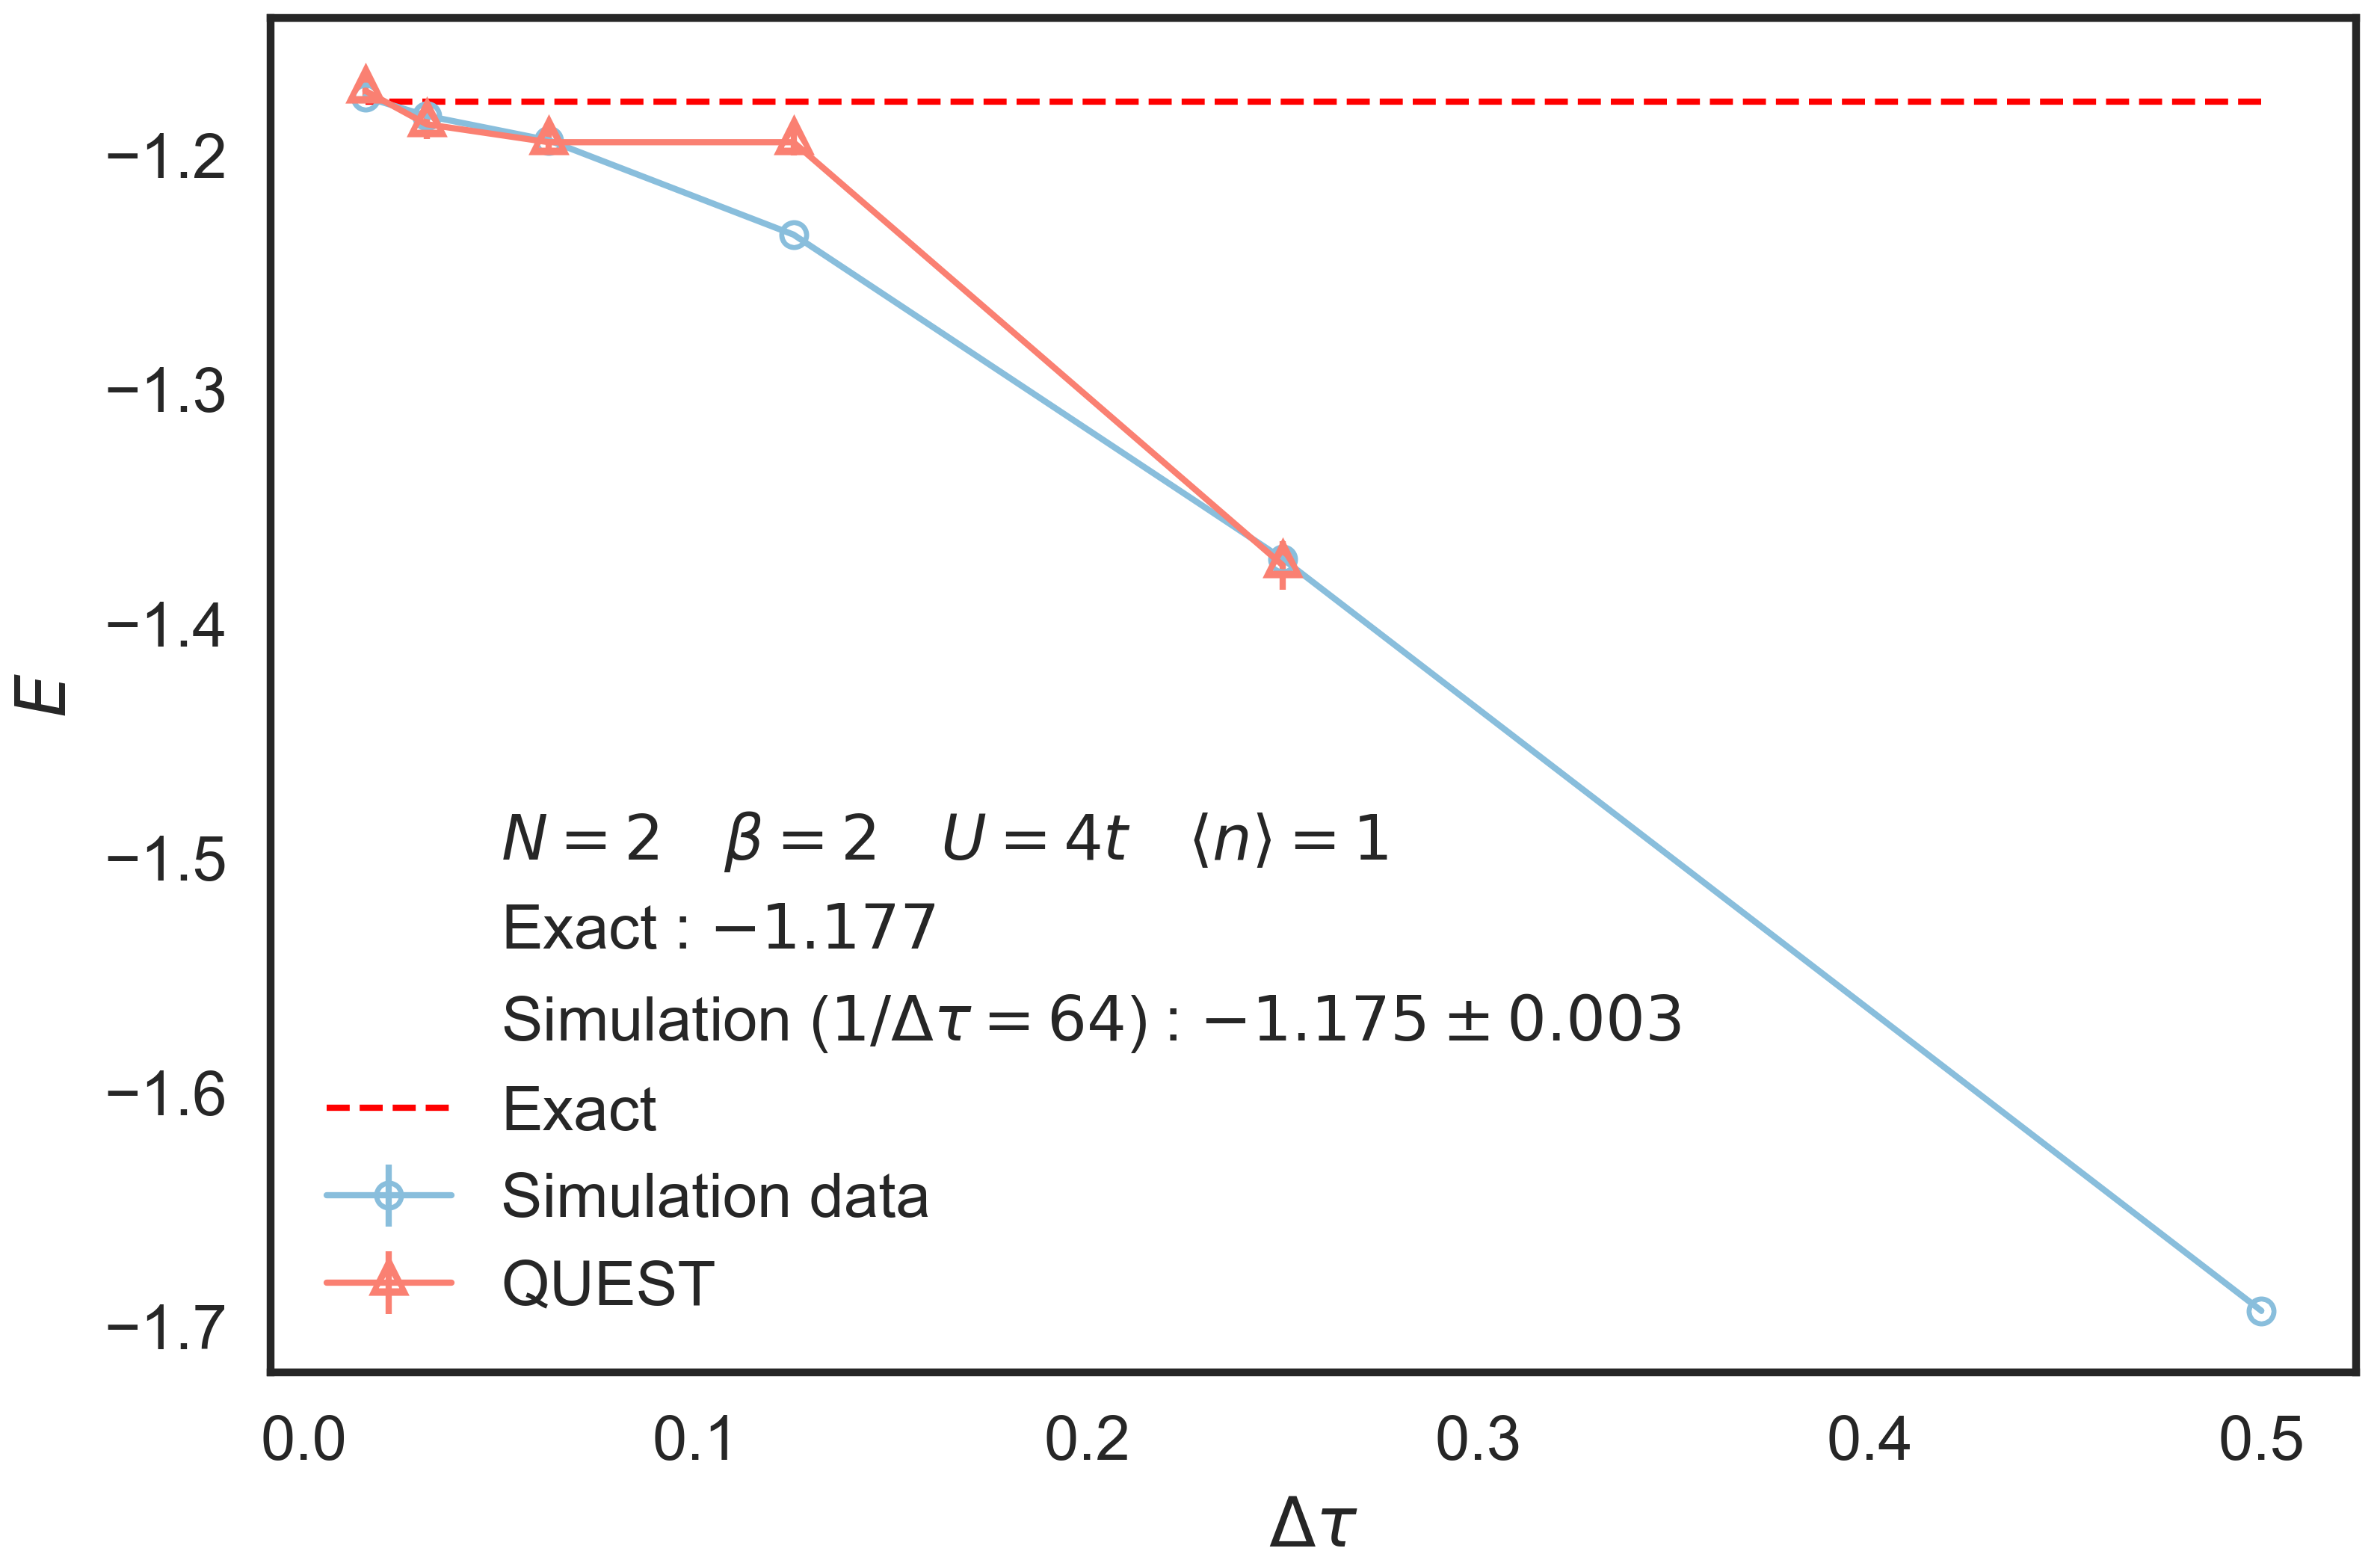
\includegraphics[scale=0.53]{Applications/Ehirsch1982.png}
\hspace{0.3cm}
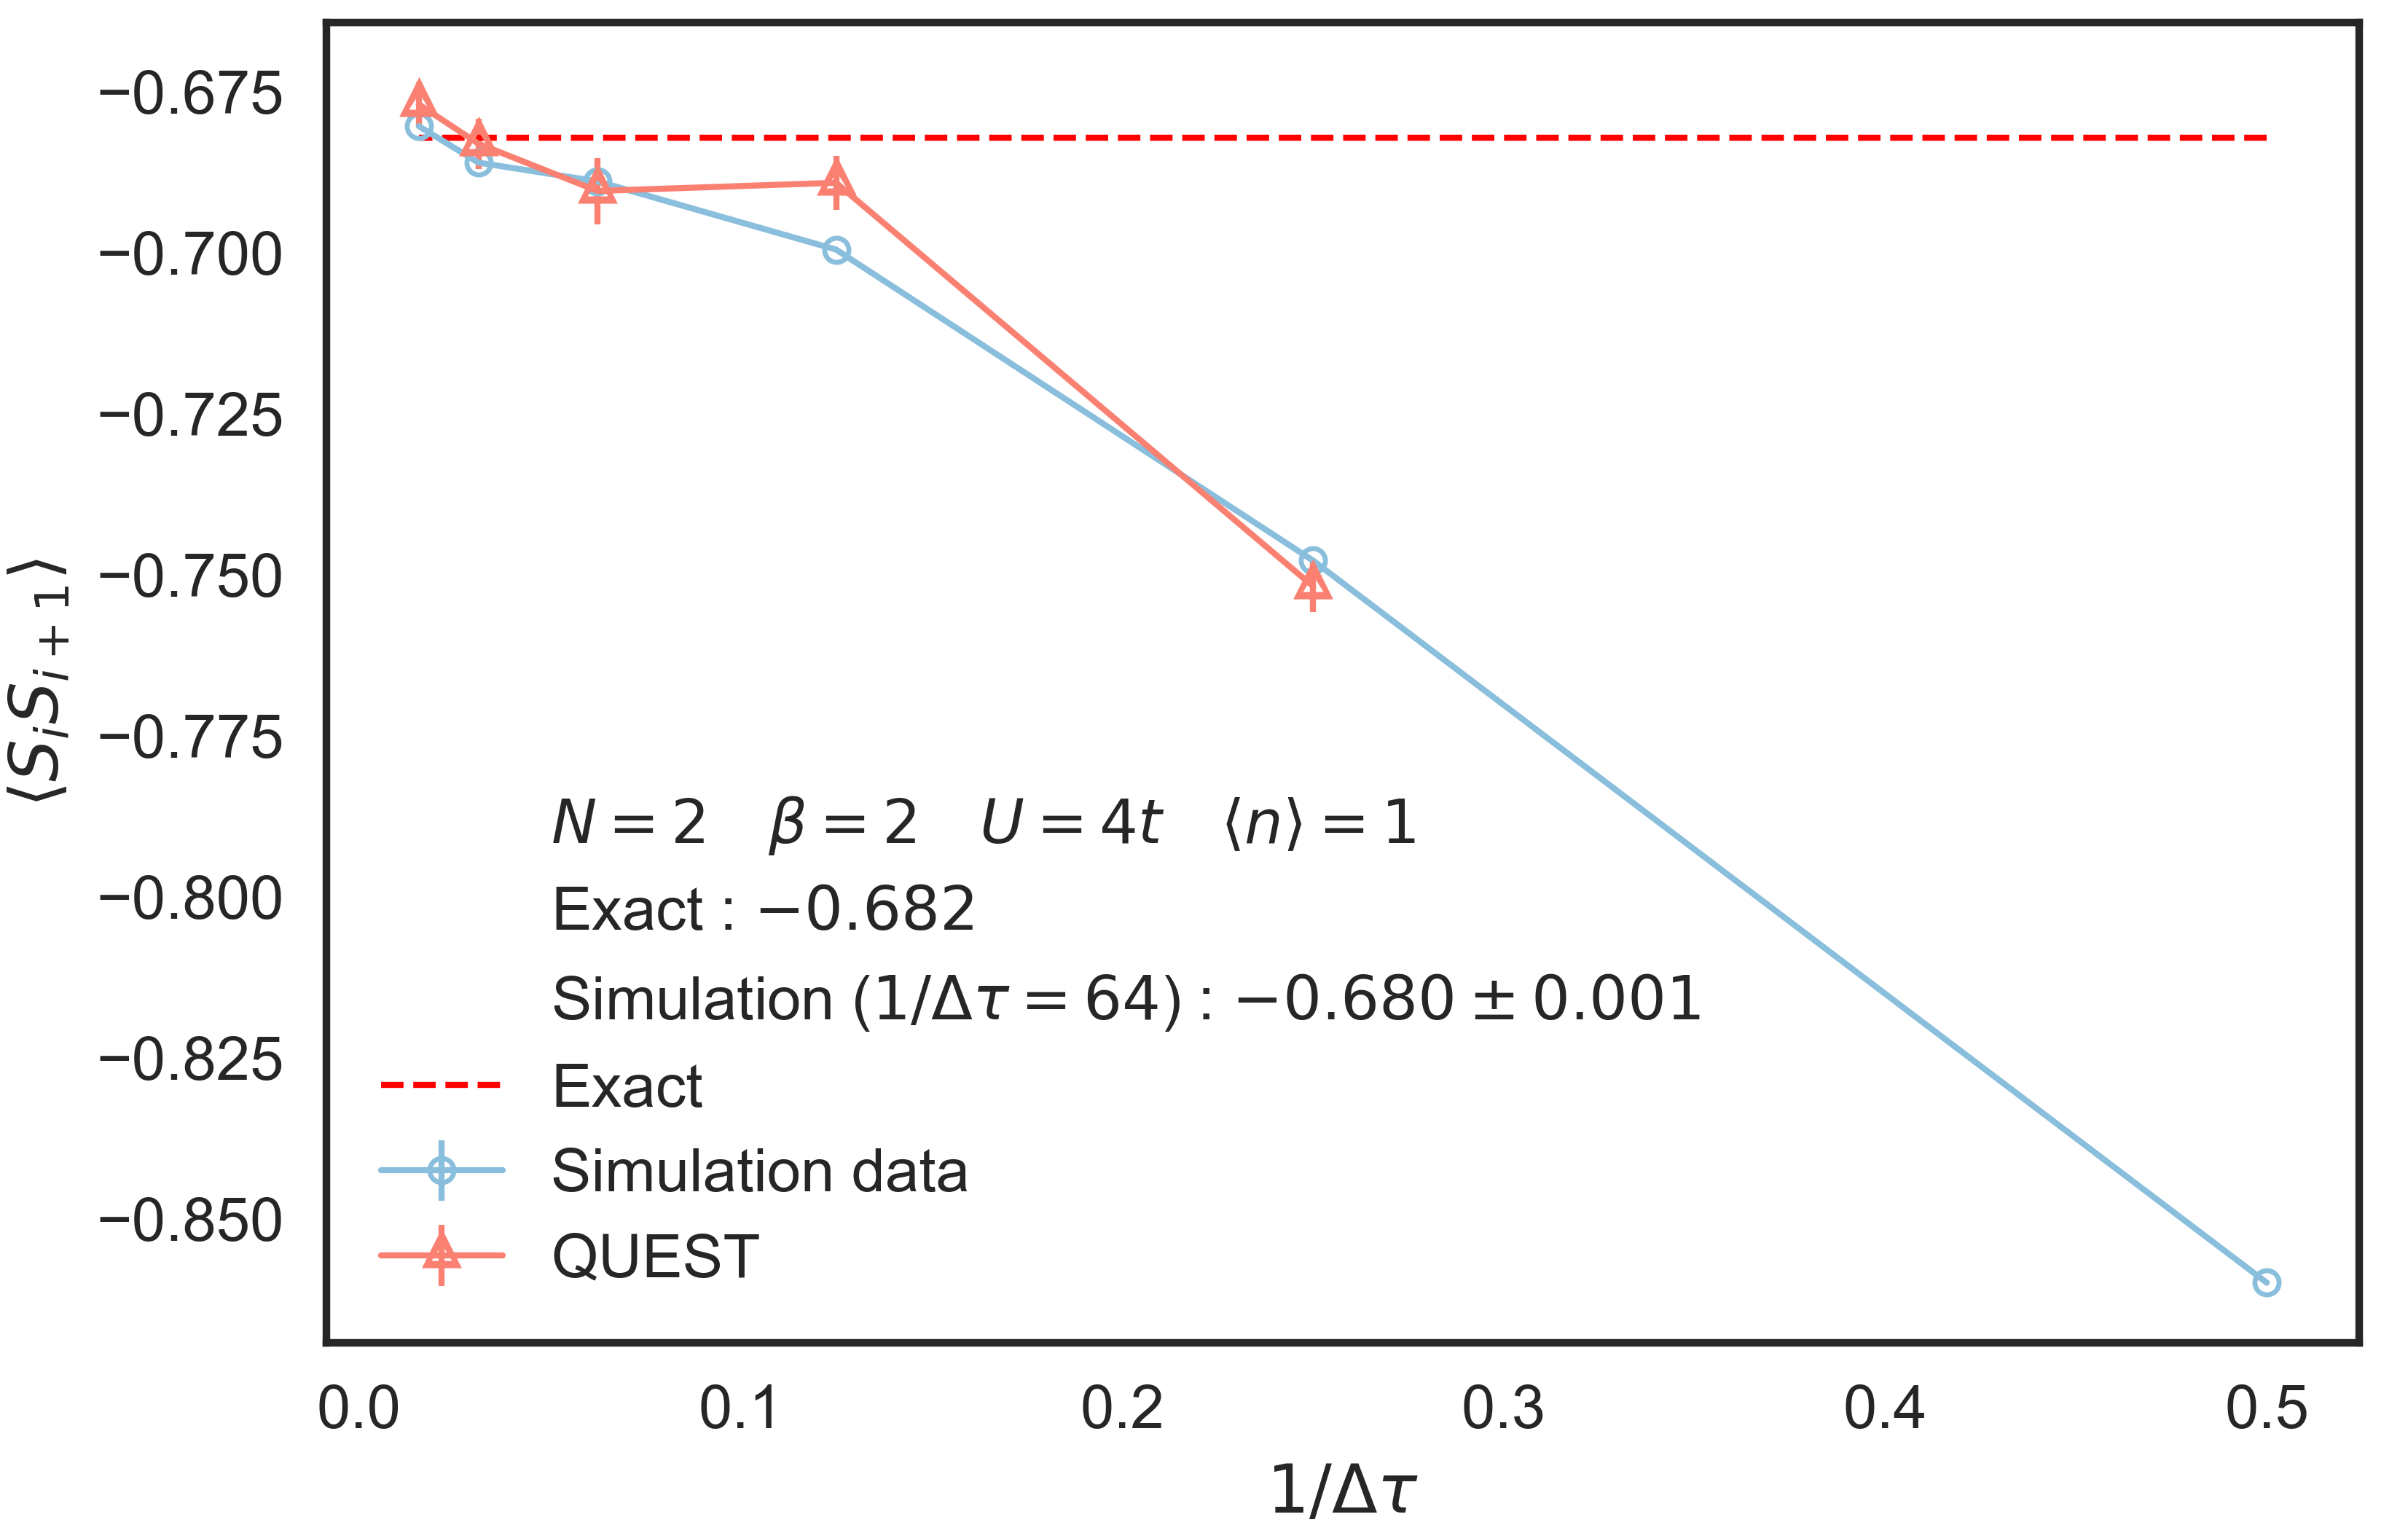
\includegraphics[scale=0.53]{Applications/SiSjhirsch1982.png}
\caption[Convergence of some of the measured observables to the value given by exact diagonalization for $N=2$, $\beta t = 2 $, $U = 4 t$.
Comparison with the results of \texttt{QUEST}.]{Convergence of some of the measured observables (left: total energy; right: spin-spin correlation) to the value given by exact diagonalization for $N=2$, $\beta t = 2 $, $U = 4 t$.
Comparison with the results of \texttt{QUEST}.\label{fig:hirsch1982}}
\end{figure}

\section{Square lattice}
\label{sec:square}

The case of the square lattice is extensively studied both at the mean field level and using \acs{QMC}.
Mean field results suggest that at half filling,  antiferromagnetic order persists even at weak coupling \cite{claveau_mean-field_2014, gouveia_magnetic_2015}, a result that we confirm with \acs{QMC}, reproducing the results of \cite{white_numerical_1989, hirsch_two-dimensional_1985}.

\begin{figure}[H]\label{fig:mfHubbardPhaseDiagram}
\hspace{0.68cm}
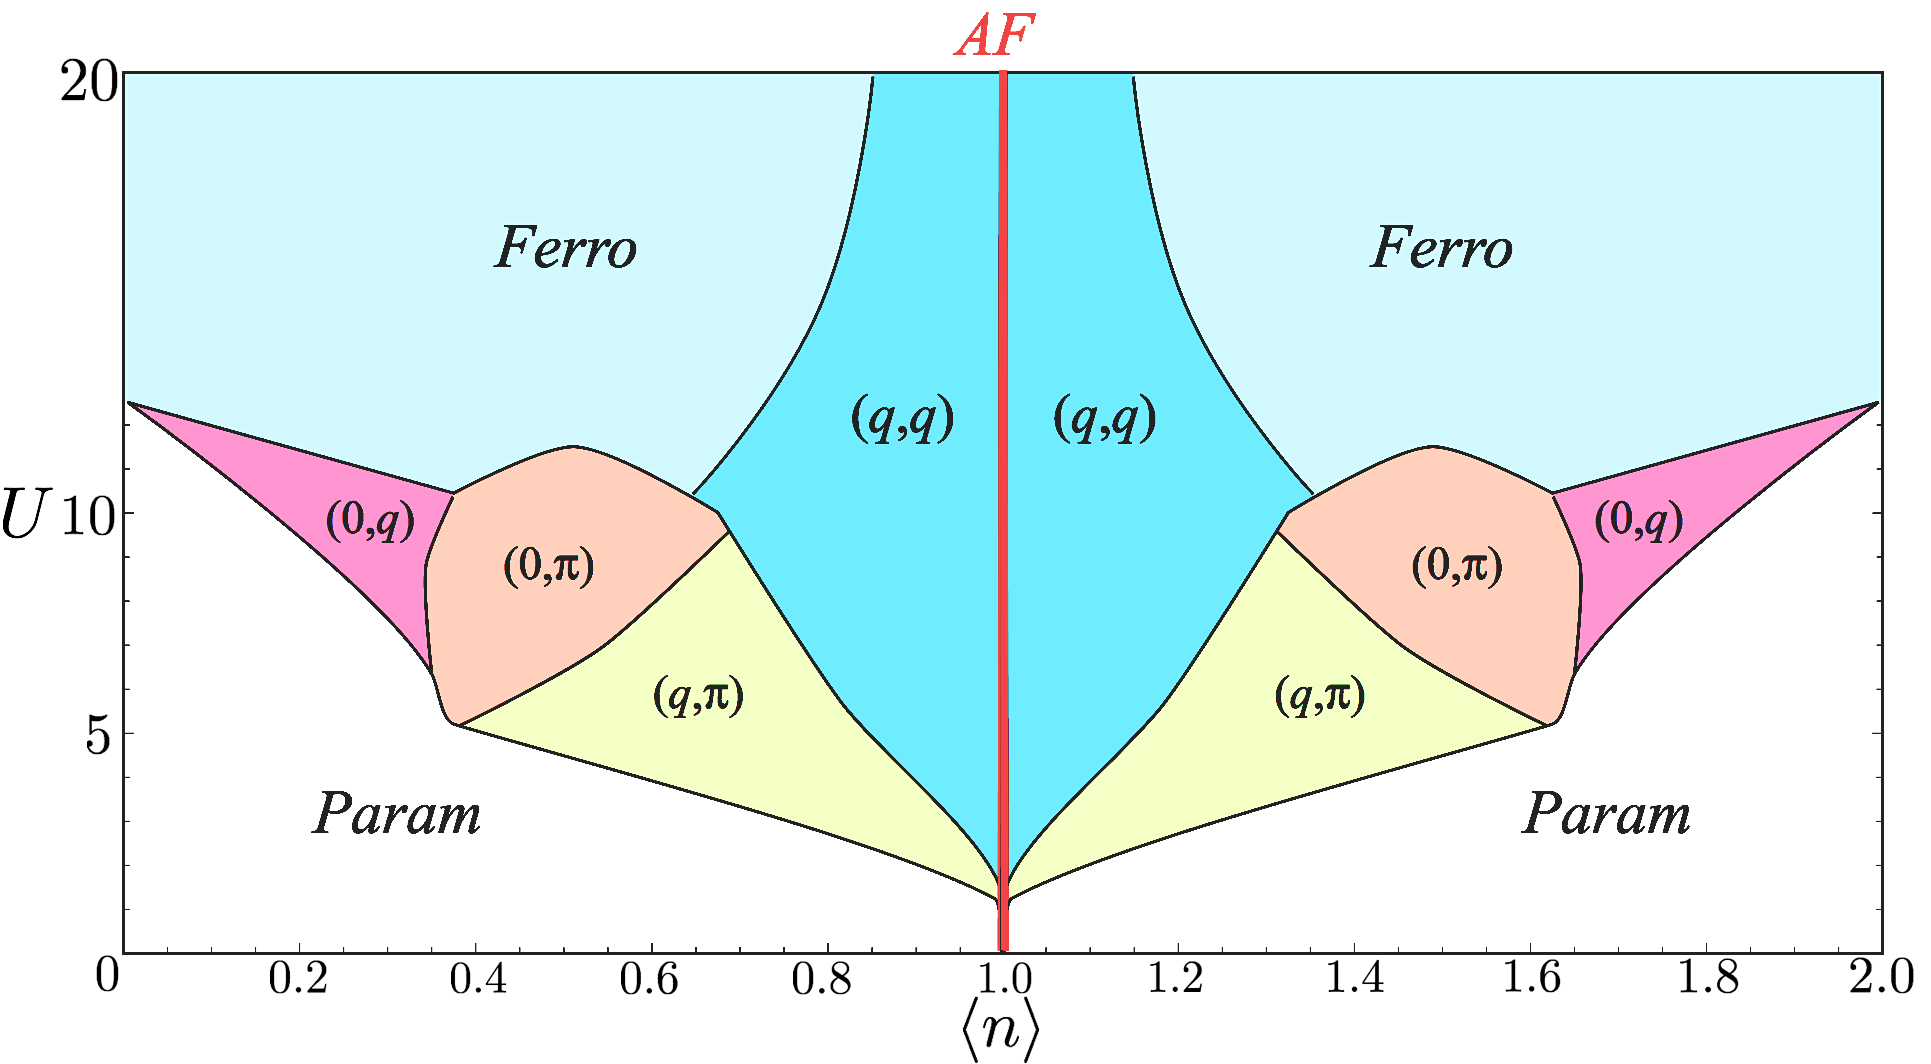
\includegraphics[scale=0.21]{Applications/mf-phase-diagram-hubbard}
\caption[]{\cite{gouveia_magnetic_2015}}
\end{figure}
\section{Honeycomb lattice}
\label{sec:honeycomb}

\section{Nanoribbons}
\label{sec:nanoribbon}

In this section, we apply our code to the case of the honeycomb lattice of graphene and of the triangular lattice with nonuniform hoppings considered in the 3-band minimal model of \acs{TMD}s.
We take boundary conditions corresponding to nanoribbons.
These structures are much longer on one direction than on the other, , i.e. $l \gg w$, resembling a ribbon, hence their name.
This condition corresponds to taking $N_x \gg N_y$ in our conventions (see Fig.(\ref{fig:bcRibbon})\footnote{In Fig.(\ref{fig:bcRibbon}), this condition is, of course, not obeyed solely for the sake of giving a good visual representation of the boundary conditions, and the numbering system).}.
The low energy electronic states on the edges of these ribbons might lead to nontrivial magnetic behavior in \ac{TMD} nanostructures (as indeed they do in graphene nanostructures \cite{yazyev_emergence_2010}) and it is this possibility was unexplored numerically before this work \cite{feldner_dynamical_2011, golor_quantum_2013}, as was mentioned on chapter \ref{cap:int}.

\subsection{Graphene}
\label{sec:graphene}

We use three coordinates to label each site on the honeycomb lattice, by taking advantage of its bipartite nature.
Regarding the honeycomb lattice as two interpenetrating triangular sublattices $\mathcal{A}$ and $\mathcal{B}$, we take the axes $x$ and $y$ to be along the primitive vectors of each triangular sublattice.
Along the $x$-direction, a ribbon is normally very long, which justifies the fact that we take \acp{PBC}.
In contrast, in the narrow $y$-direction we take \acp{OBC}.
To number the sites on the ribbon, we introduce an additional coordinate labeling the sublattice: $z = 0$, if the site is in sublattice $\mathcal{A}$, and $z = 1$ if the site is in sublattice $\mathcal{B}$.
We then adopt the numbering convention for the sites $i = 0,1, ..., 2 N_x N_y - 1$ of the lattice $\mathcal{L}$:
$
i (x, y, z) = N_x N_y z + N_x y + x,
$
 where $x = 0, ..., N_x - 1$, $y = 0, ..., N_y - 1$, and $z = 0, 1$ define each element $\bm r = (x, y, z) \in \mathcal{L}$.

\begin{figure}[H]
\hspace{-0.4cm}
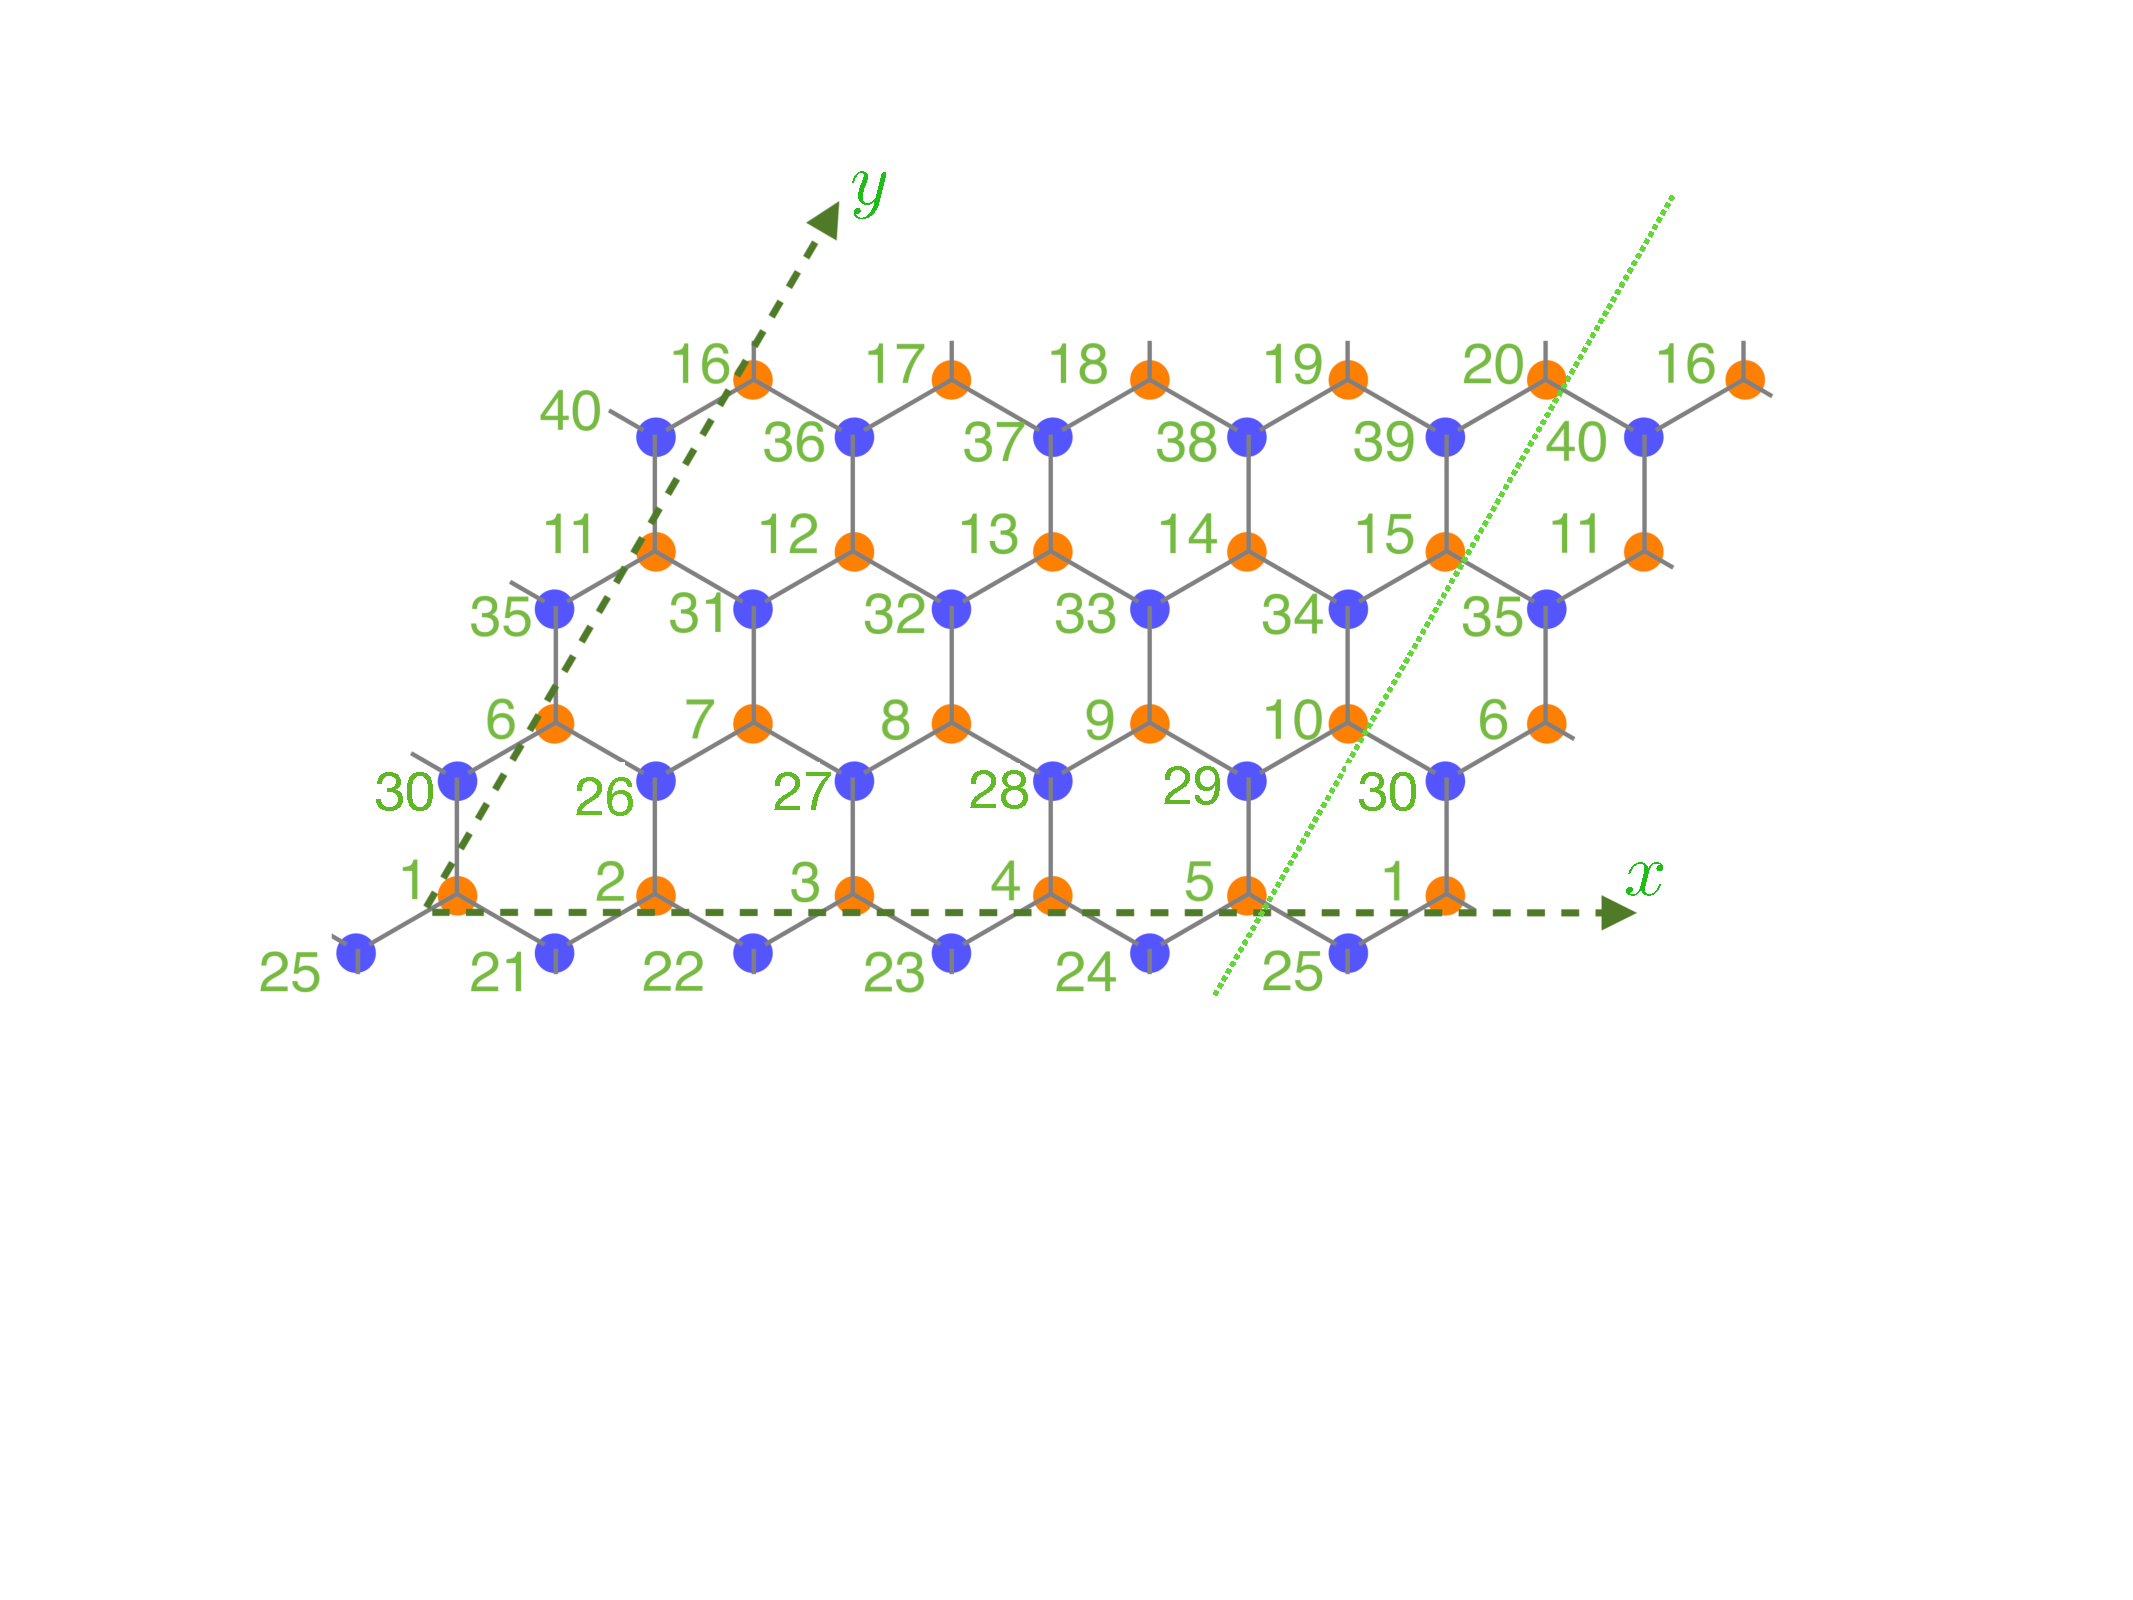
\includegraphics[trim={0 8cm 0 2.5cm},clip, scale = 0.27]{Applications/nanoribbon.pdf}
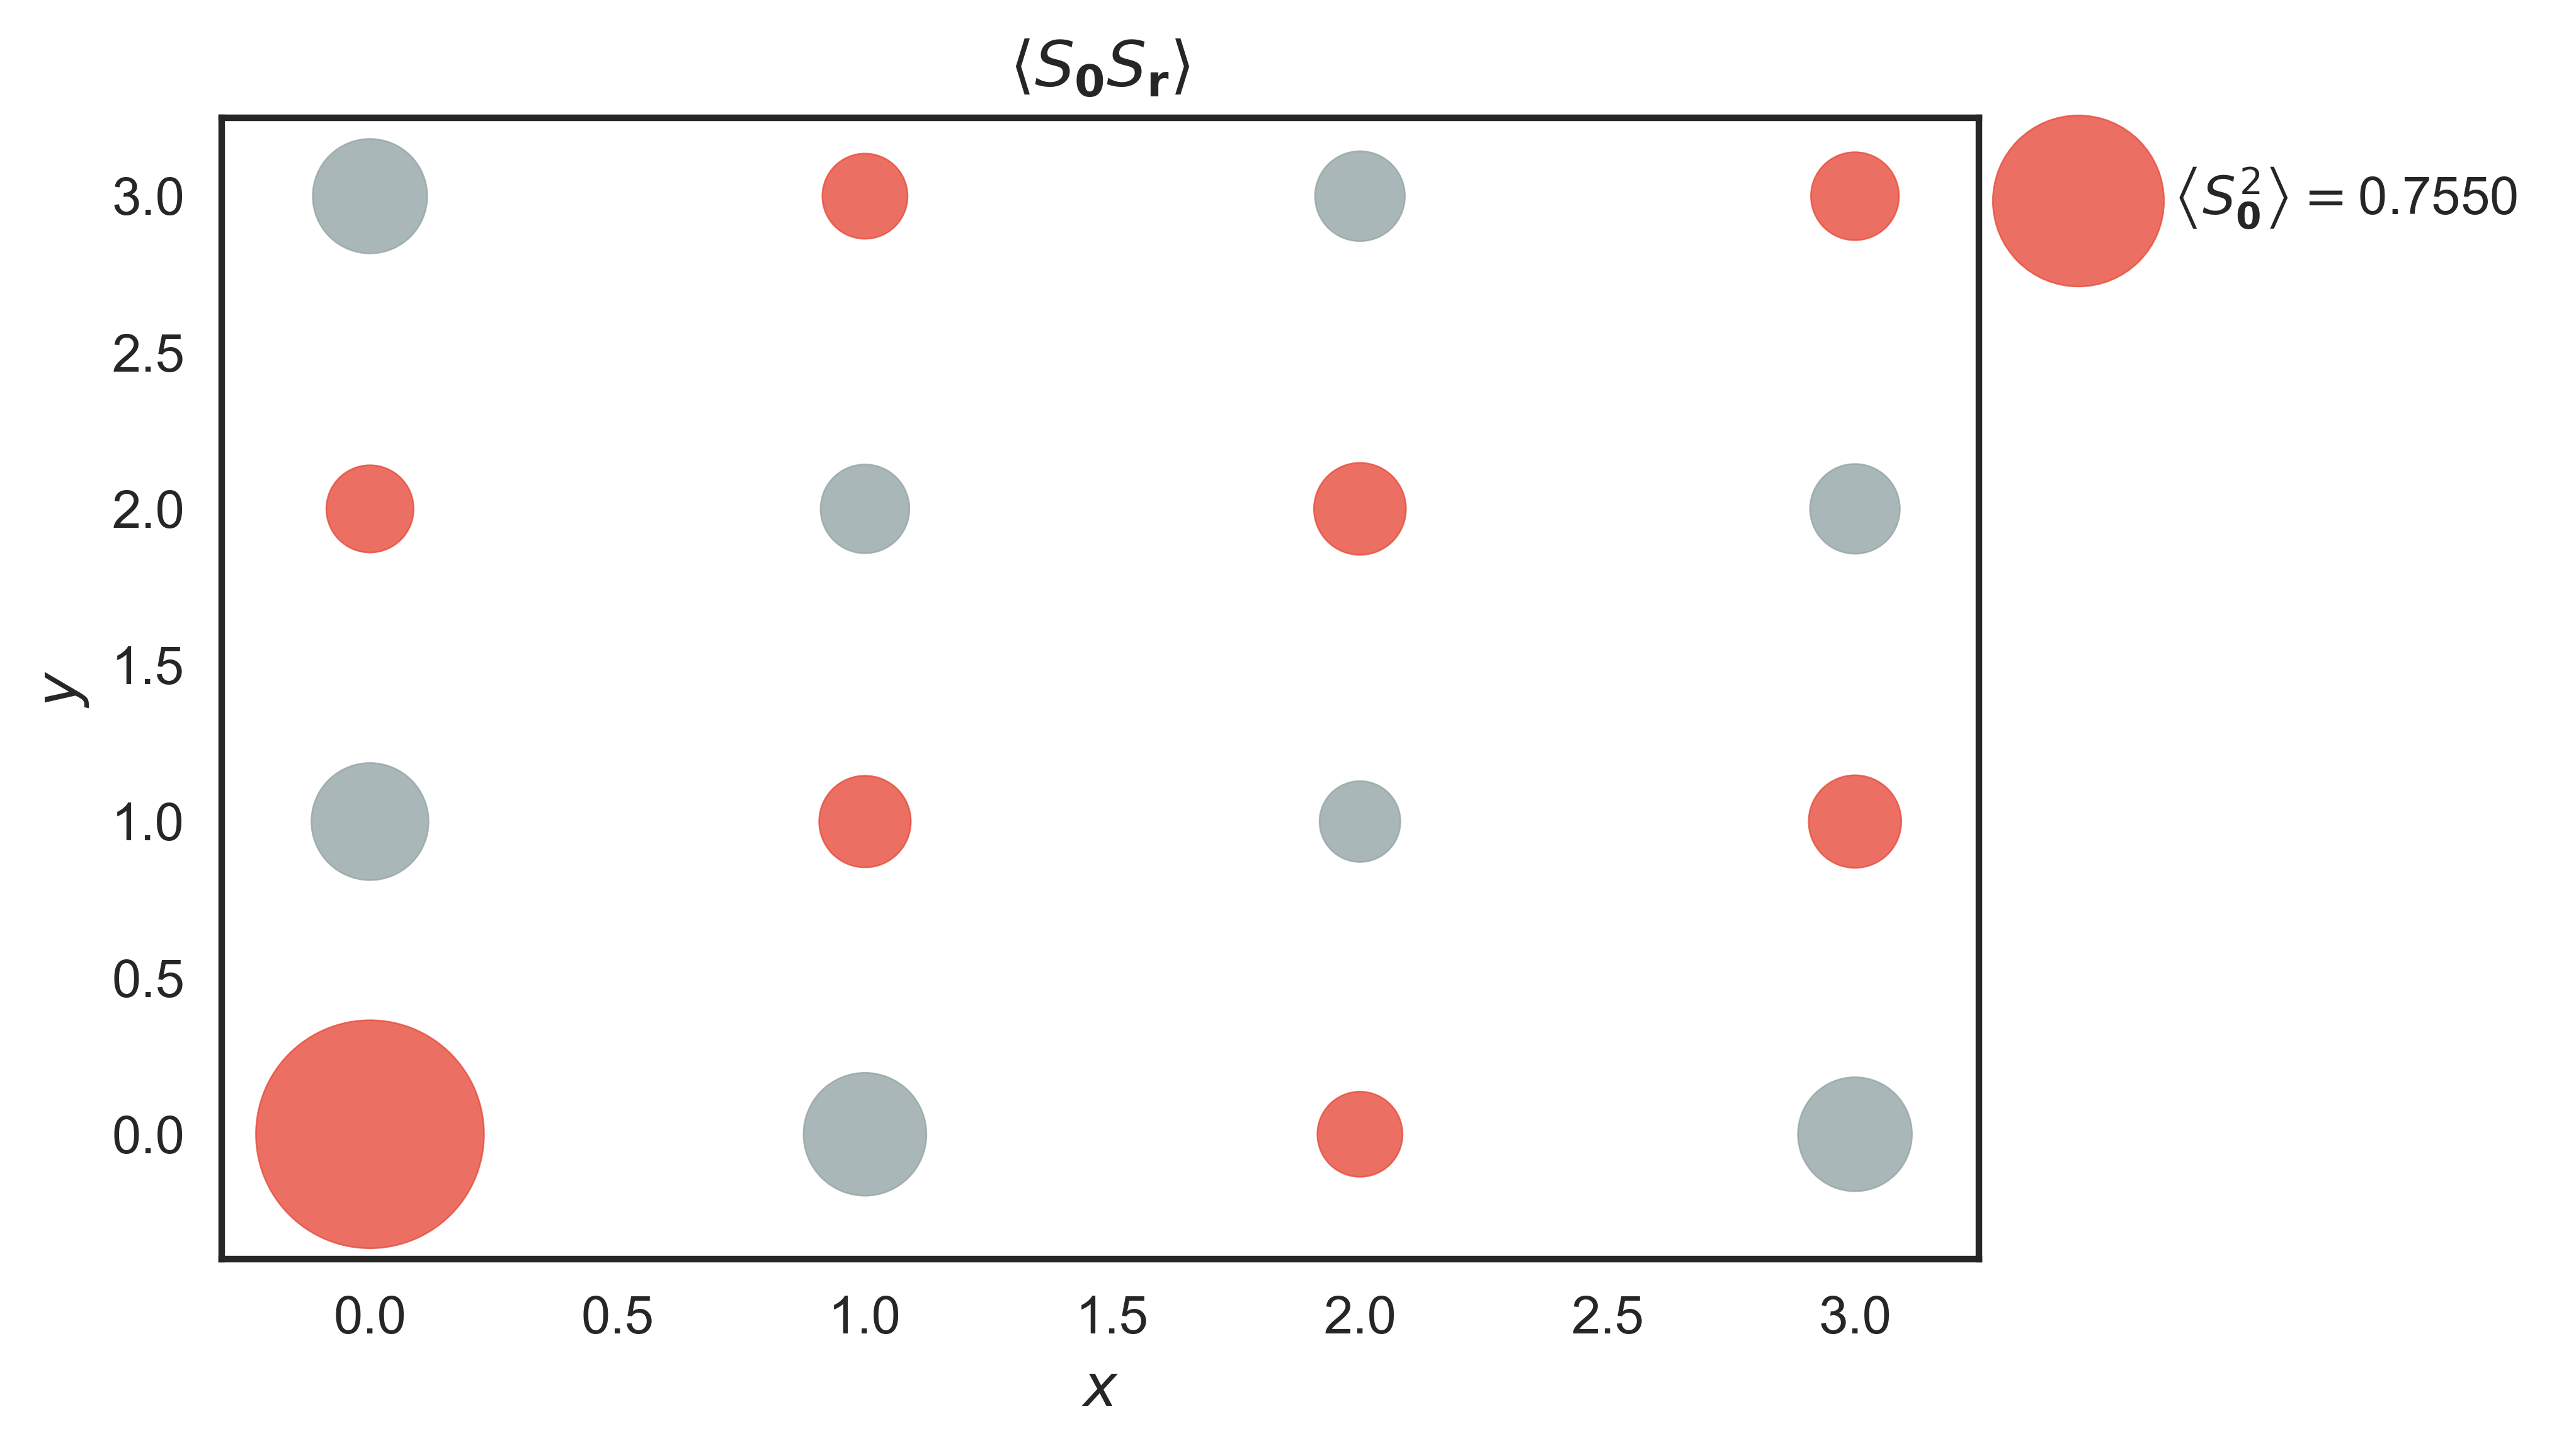
\includegraphics[scale = 0.49]{Applications/graphene-strain/CorrelationsDots.png}
	\caption[Boundary conditions on the nanoribbon.]{Boundary conditions on the nanoribbon for $N_x = 5, \, N_y = 4$. The orange circles correspond to sublattice $\mathcal{A}$, and the blue circles correspond to sublattice $\mathcal{B}$.
	The counting starts at 1 (i.e. the numbers correspond to $i+1$, since $i$ starts at 0).}
	\label{fig:bcRibbon}
\end{figure}

The geometry of the system appears through the hopping matrix $\bm K$ in our code.
This numbering system makes it straightforward to find the neighbors of each site.
Let us begin by considering a site that is not on a zigzag edge.
There are two possible cases. For example, for 
$
z_i = 0, y_i \neq N_y - 1, x_i \neq 0 ,
$
 we have that the nearest neighbors of $i$ are $ j (i) = \{ j ( \bm r) \}$, with $\bm r$ in
\begin{equation*}
\bigg\{ \bm r_j \in \mathcal{L} \bigg| z_j = 1 \,\land\, \bigg[ \bigg( y_j = y_i  \,\land\, ( x_j = x_i \,\lor\, x_j = x_i - 1) \bigg) \,\lor\, \bigg( y_j = y_i + 1  \,\land\, x_j = x_i - 1  \bigg)  \bigg] \bigg\}
\end{equation*}

As opposed to the sites of a honeycomb lattice with \acp{PBC}, which have 3 neighbors, the sites of the zigzag edges have only 2 neighbors.
We summarize all possible cases in the following table.

\begin{table}[H]
\centering
	\caption{Nearest neighbors on the graphene nanoribbon.
	The neighbors in gray are only for sites that are not on the edges.
	$\%$ refers to the remainder of integer division.}
	\begin{tabular}{|c|c|c|c|} \hline
	\multicolumn{4}{|c|}{\textbf{\acp{OBC} \color{silver}{(\acp{PBC})} }}							\\ \hline
		Case 				& $z_j$	& $y_j$	& $x_j$ 	\\ \hline
		\multicolumn{1}{|c|}{\multirow{3}{*}{$z_i = 0$}}	 &	\multicolumn{1}{c|}{\multirow{3}{*}{1}} & \multicolumn{1}{c|}{\multirow{2}{*}{$y_i$}} & $x_i$   \\ \cline{4-4}
	   	\multicolumn{1}{|c|}{}	& \multicolumn{1}{c|}{\multirow{3}{*}{}} & \multicolumn{1}{c|}{\multirow{2}{*}{}}& \multicolumn{1}{c|}{\multirow{2}{*}{$N_x - 1 - (N_x - x_i) \% N_x$}} \\ \cline{3-3}
	   	\multicolumn{1}{|c|}{}	& \multicolumn{1}{c|}{} & \color{silver}{$y_i +1$} & \multicolumn{1}{c|}{\multirow{2}{*}{}} \\ \hline
		\multicolumn{1}{|c|}{\multirow{3}{*}{$z_i = 1$}}	 &	\multicolumn{1}{c|}{\multirow{3}{*}{0}} & \multicolumn{1}{c|}{\multirow{2}{*}{$y_i$}} & $x_i$   \\ \cline{4-4}
	   	\multicolumn{1}{|c|}{}	& \multicolumn{1}{c|}{\multirow{3}{*}{}} & \multicolumn{1}{c|}{\multirow{2}{*}{}}& \multicolumn{1}{c|}{\multirow{2}{*}{$(x_i + 1) \% N_x$}} \\ \cline{3-3}
	   	\multicolumn{1}{|c|}{}	& \multicolumn{1}{c|}{} & \color{silver}{$y_i -1$} & \multicolumn{1}{c|}{\multirow{2}{*}{}} \\ \hline
	\end{tabular}
	\label{tab:dummytable}
\end{table}

\begin{figure}[H]
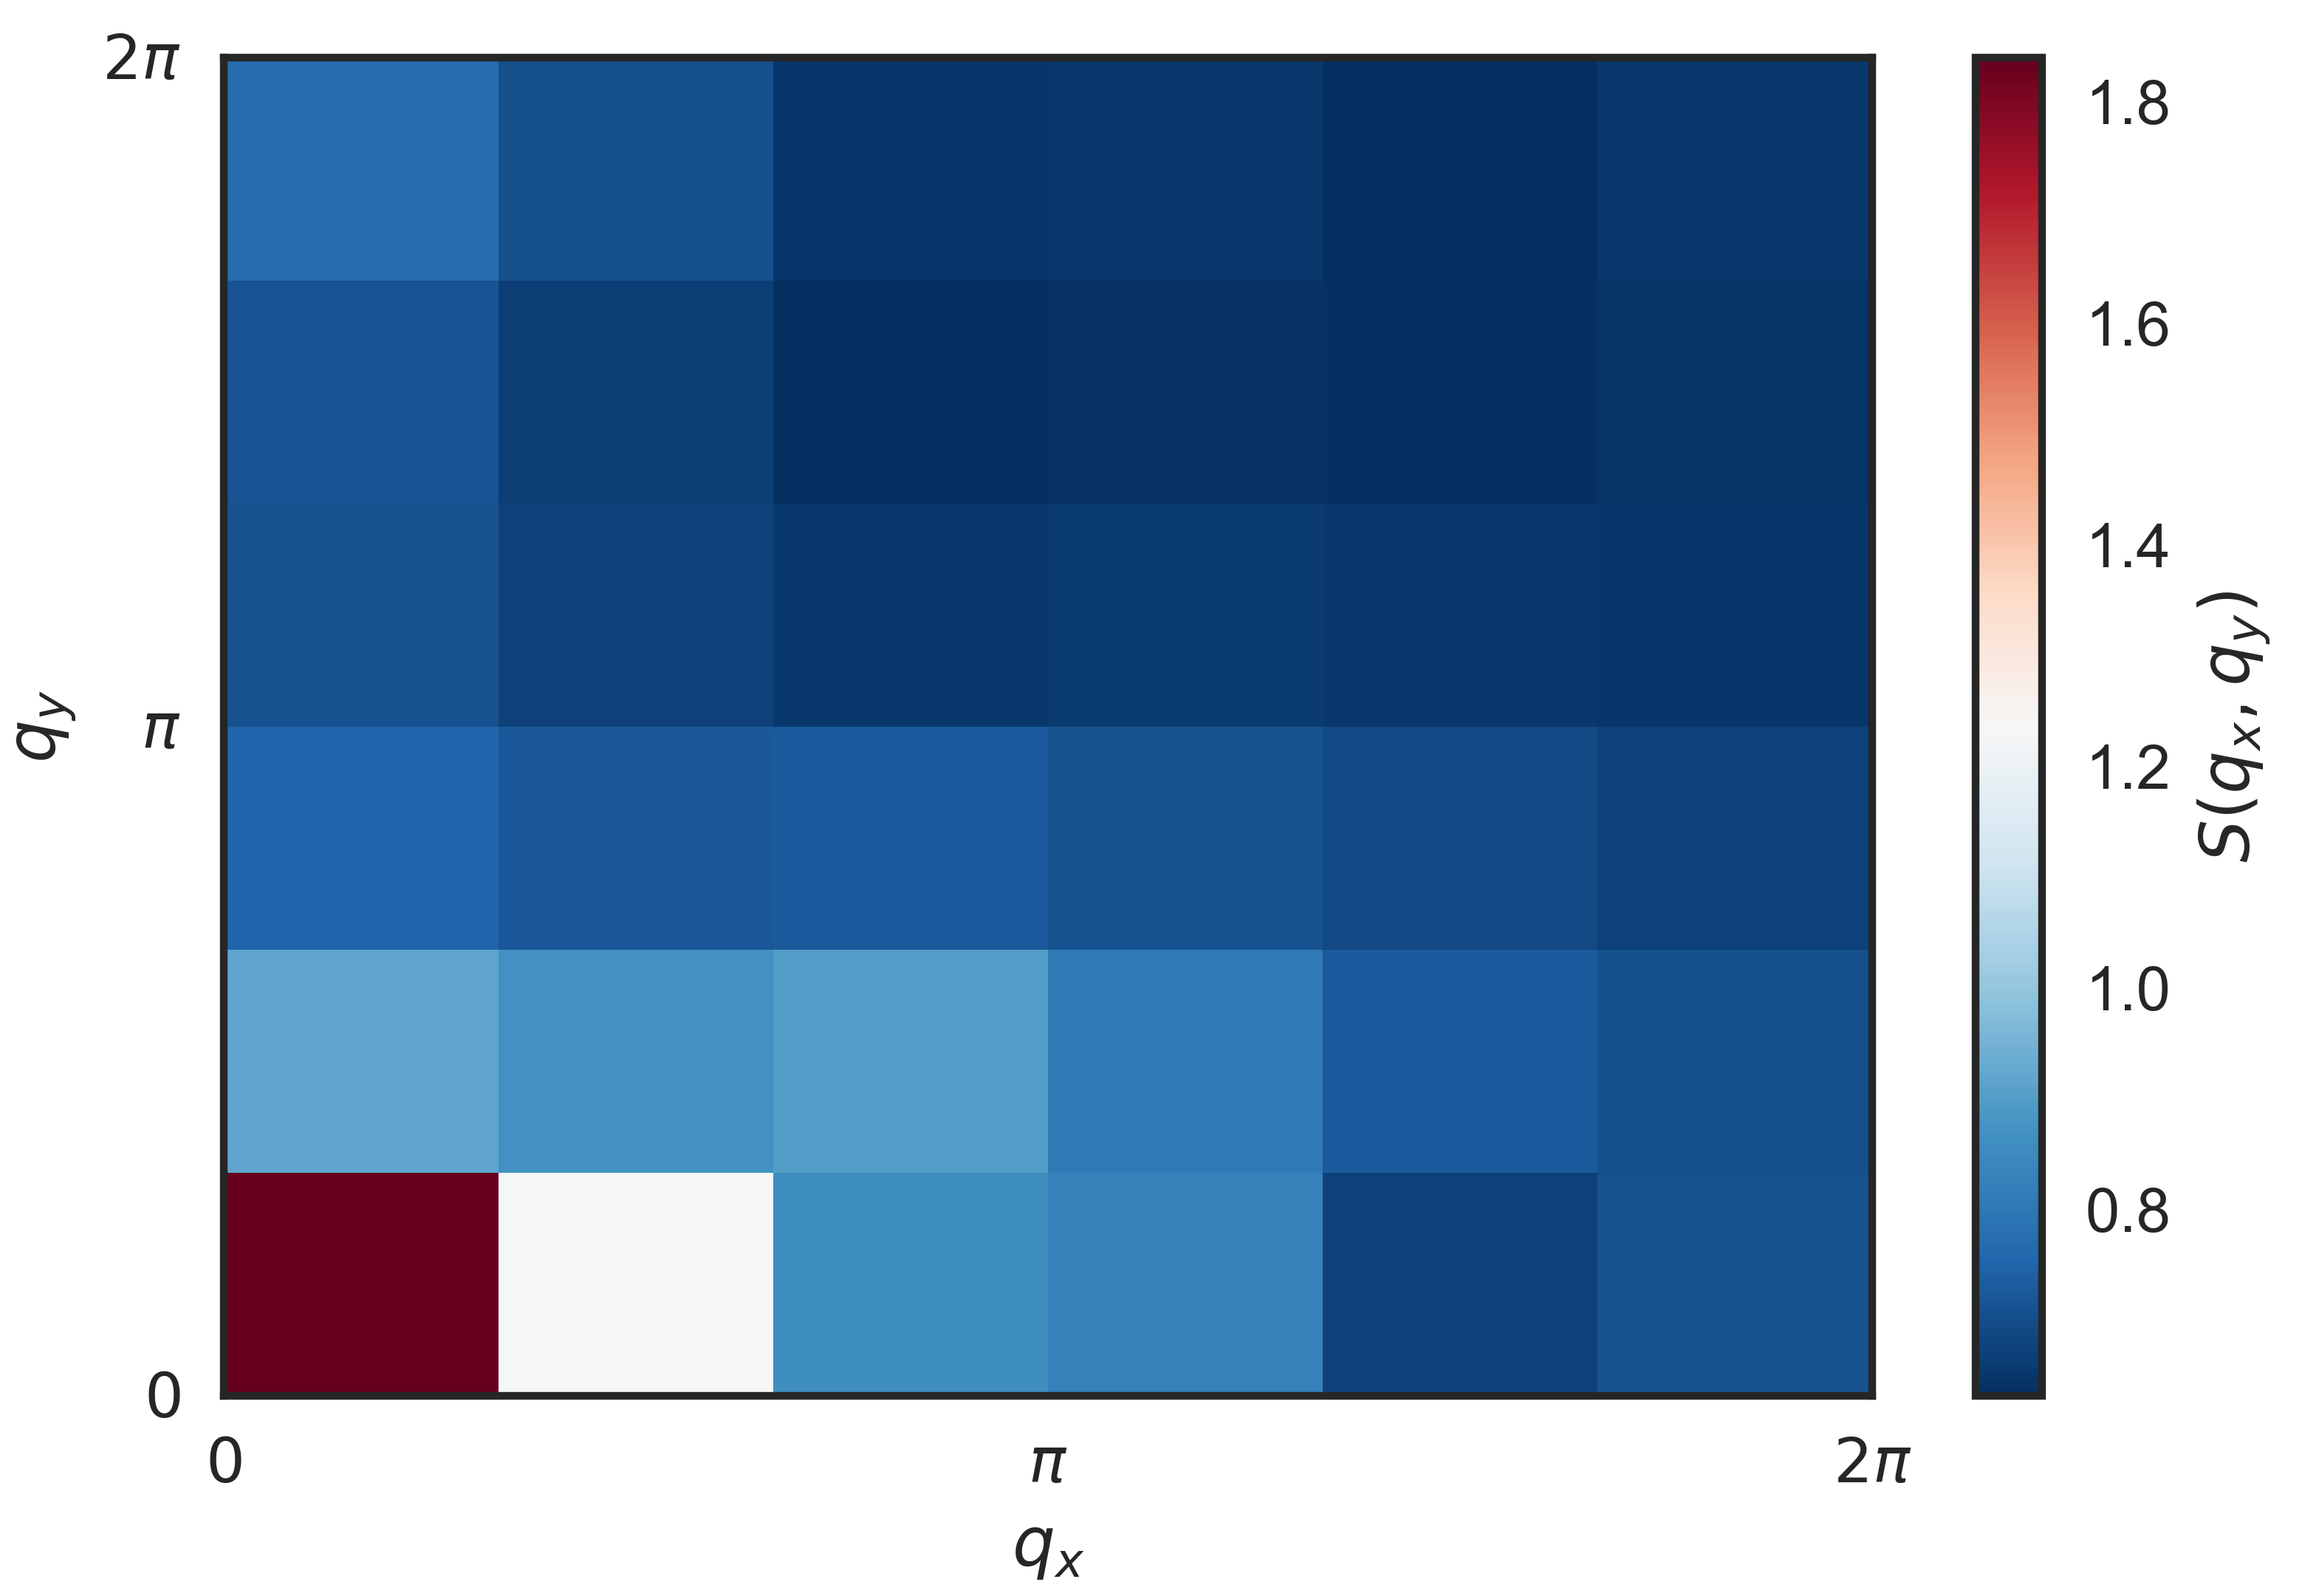
\includegraphics[scale = 0.56]{Applications/graphene-strain/S(q)pcolor.png}
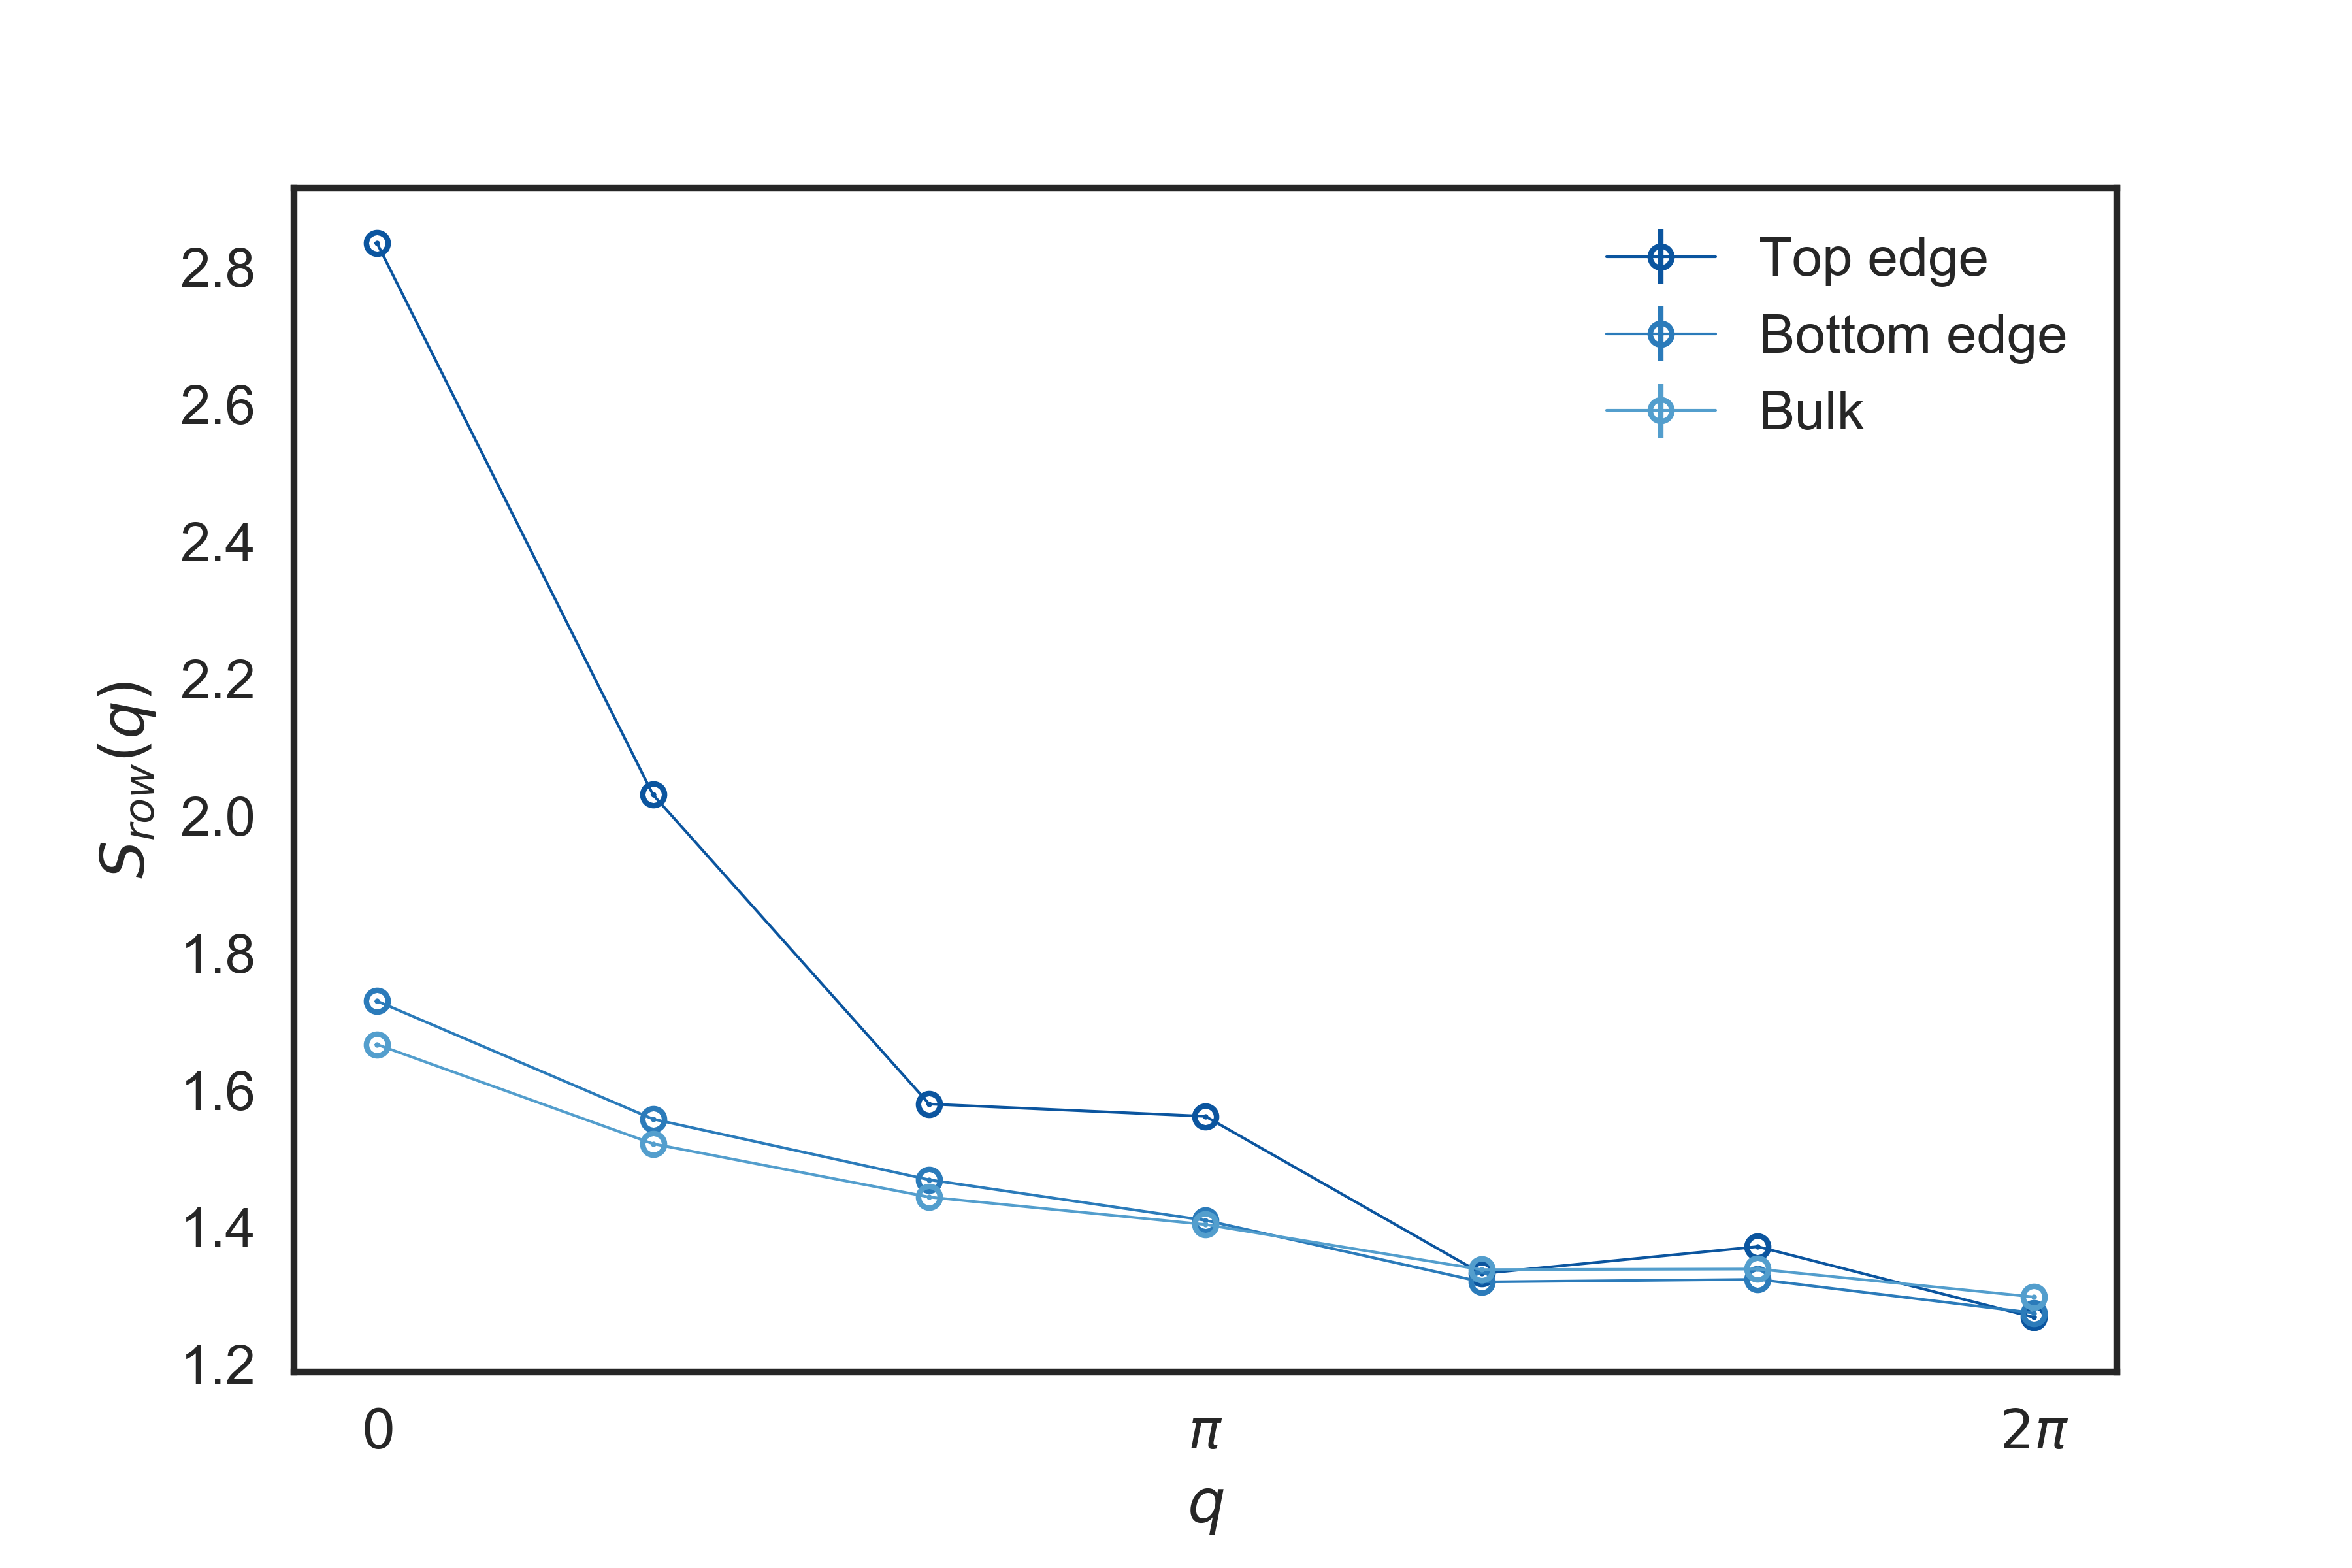
\includegraphics[scale = 0.55]{Applications/graphene-strain/edgeStFactor_Graphene.png}
	\caption[]{}
	\label{fig:edgeStFactor}
\end{figure}
\begin{figure}[H]
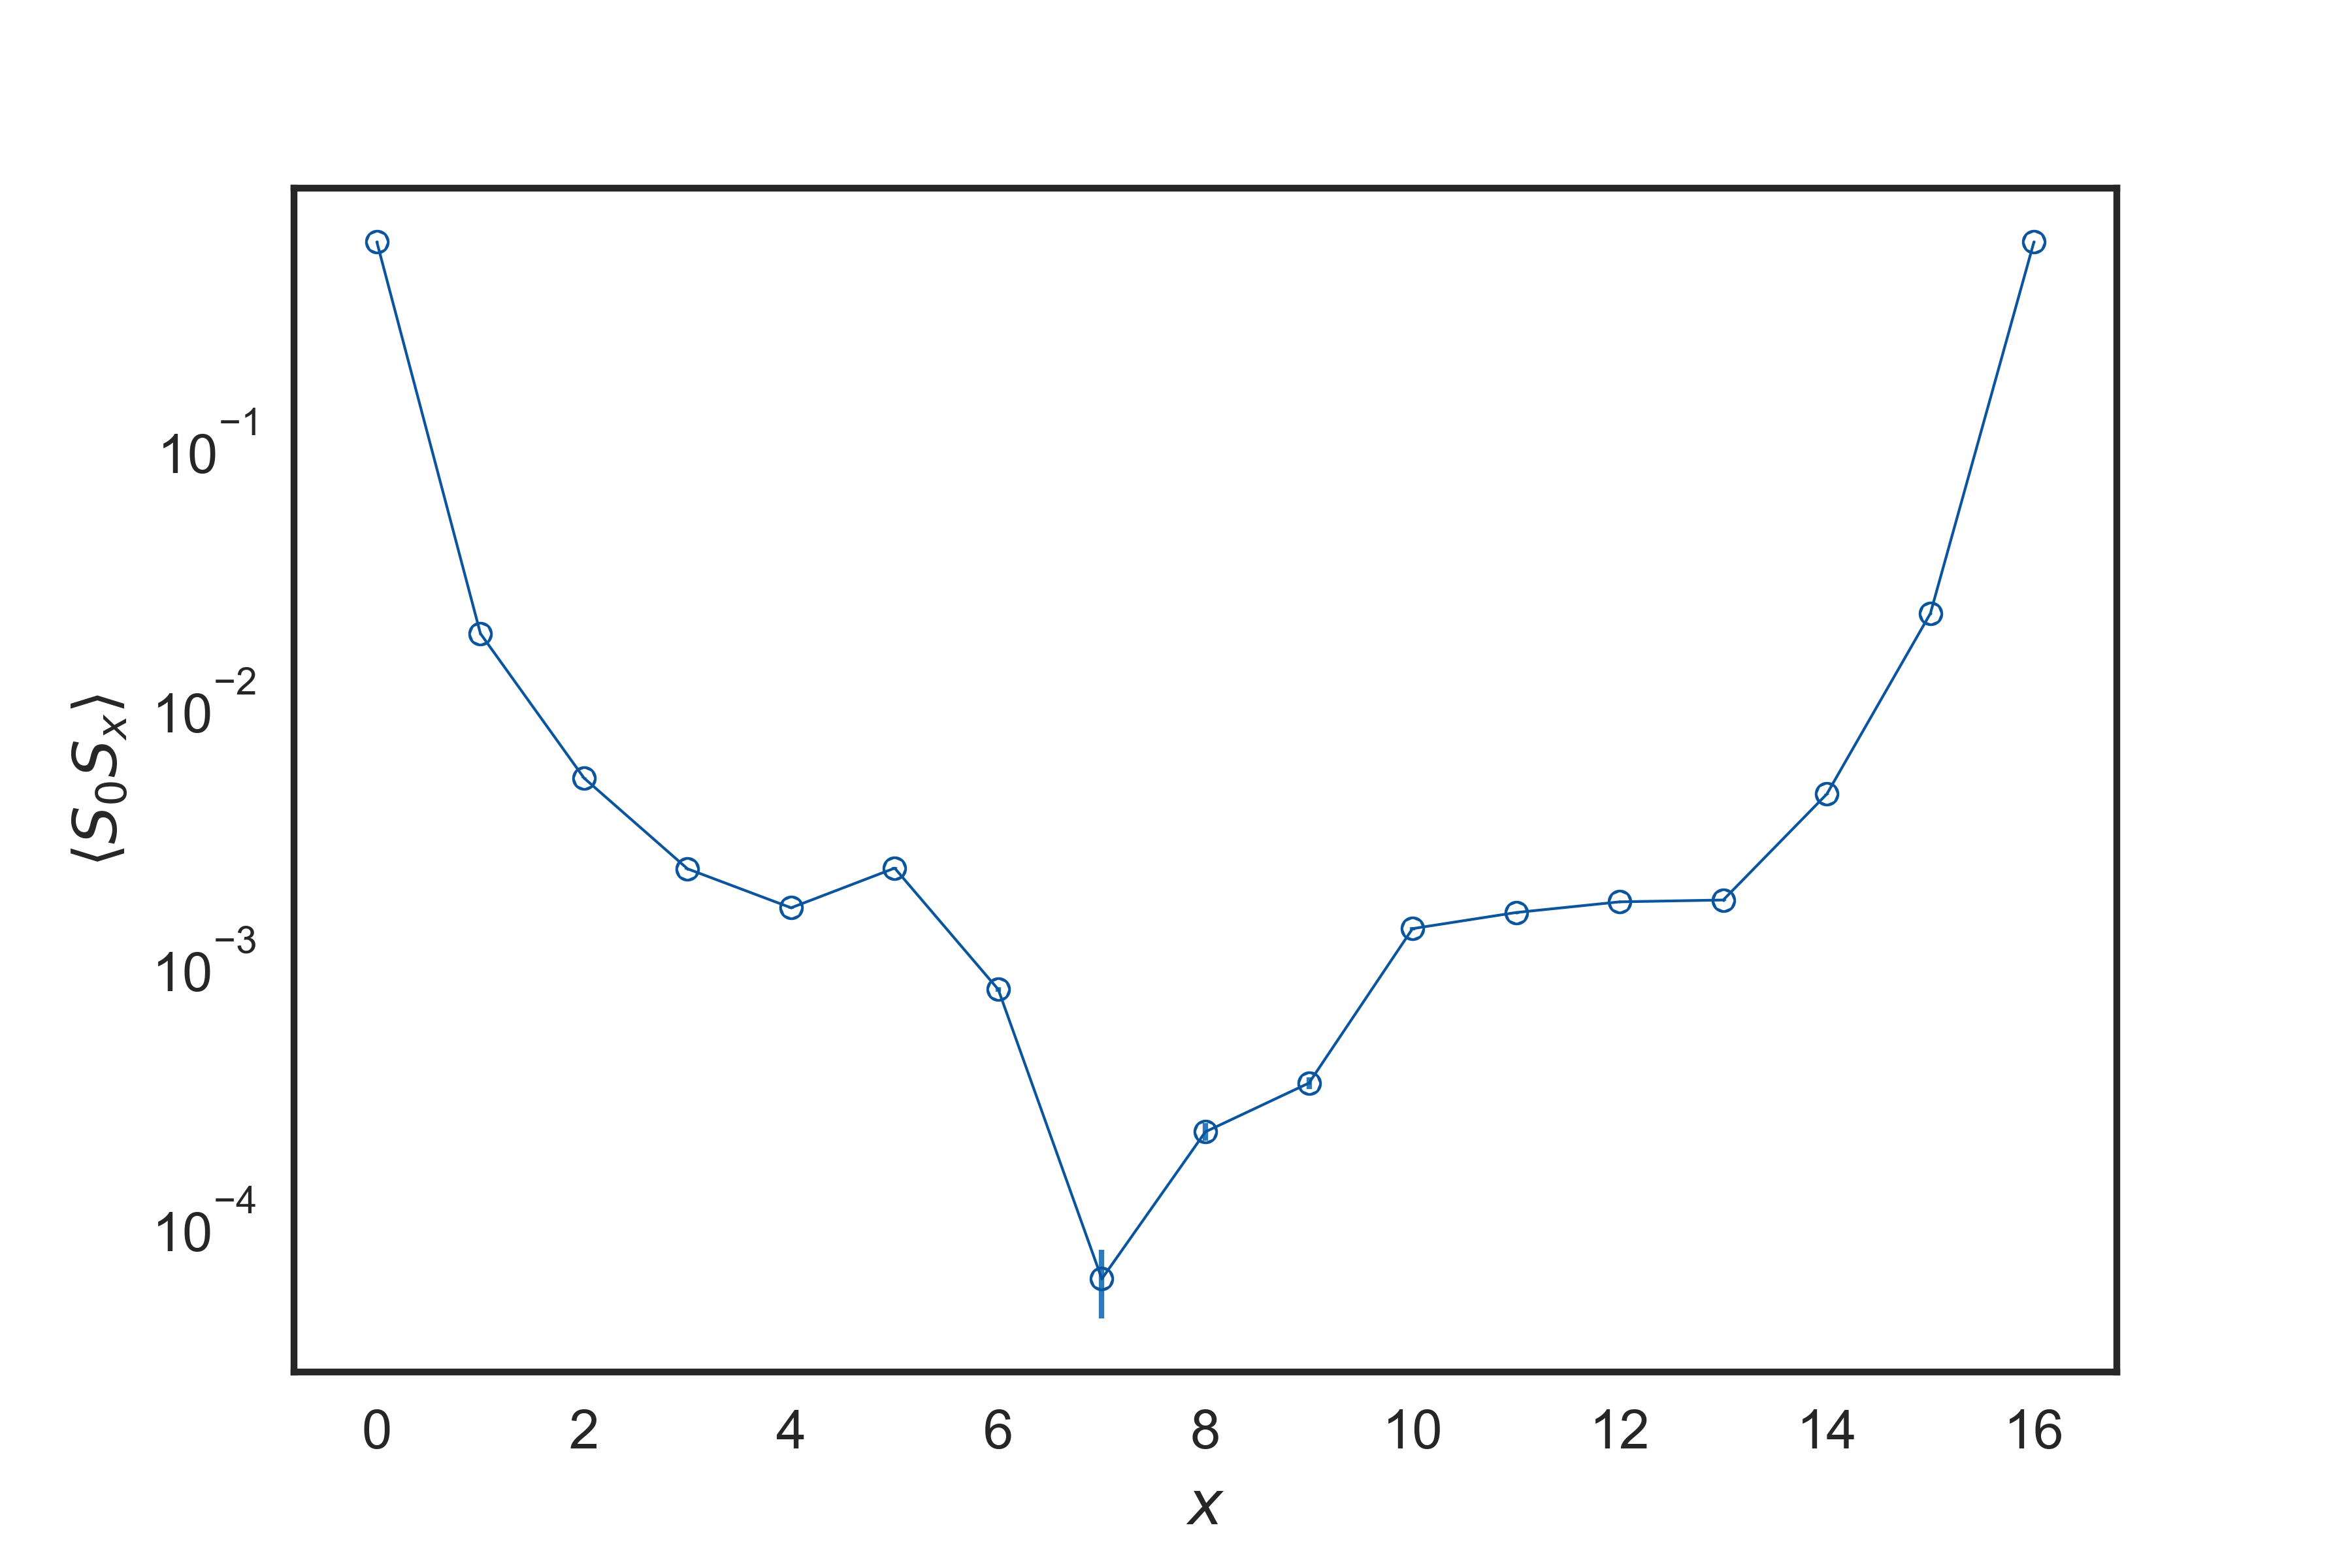
\includegraphics[scale = 0.55]{Applications/graphene-strain/LongitudinalProfile.png}
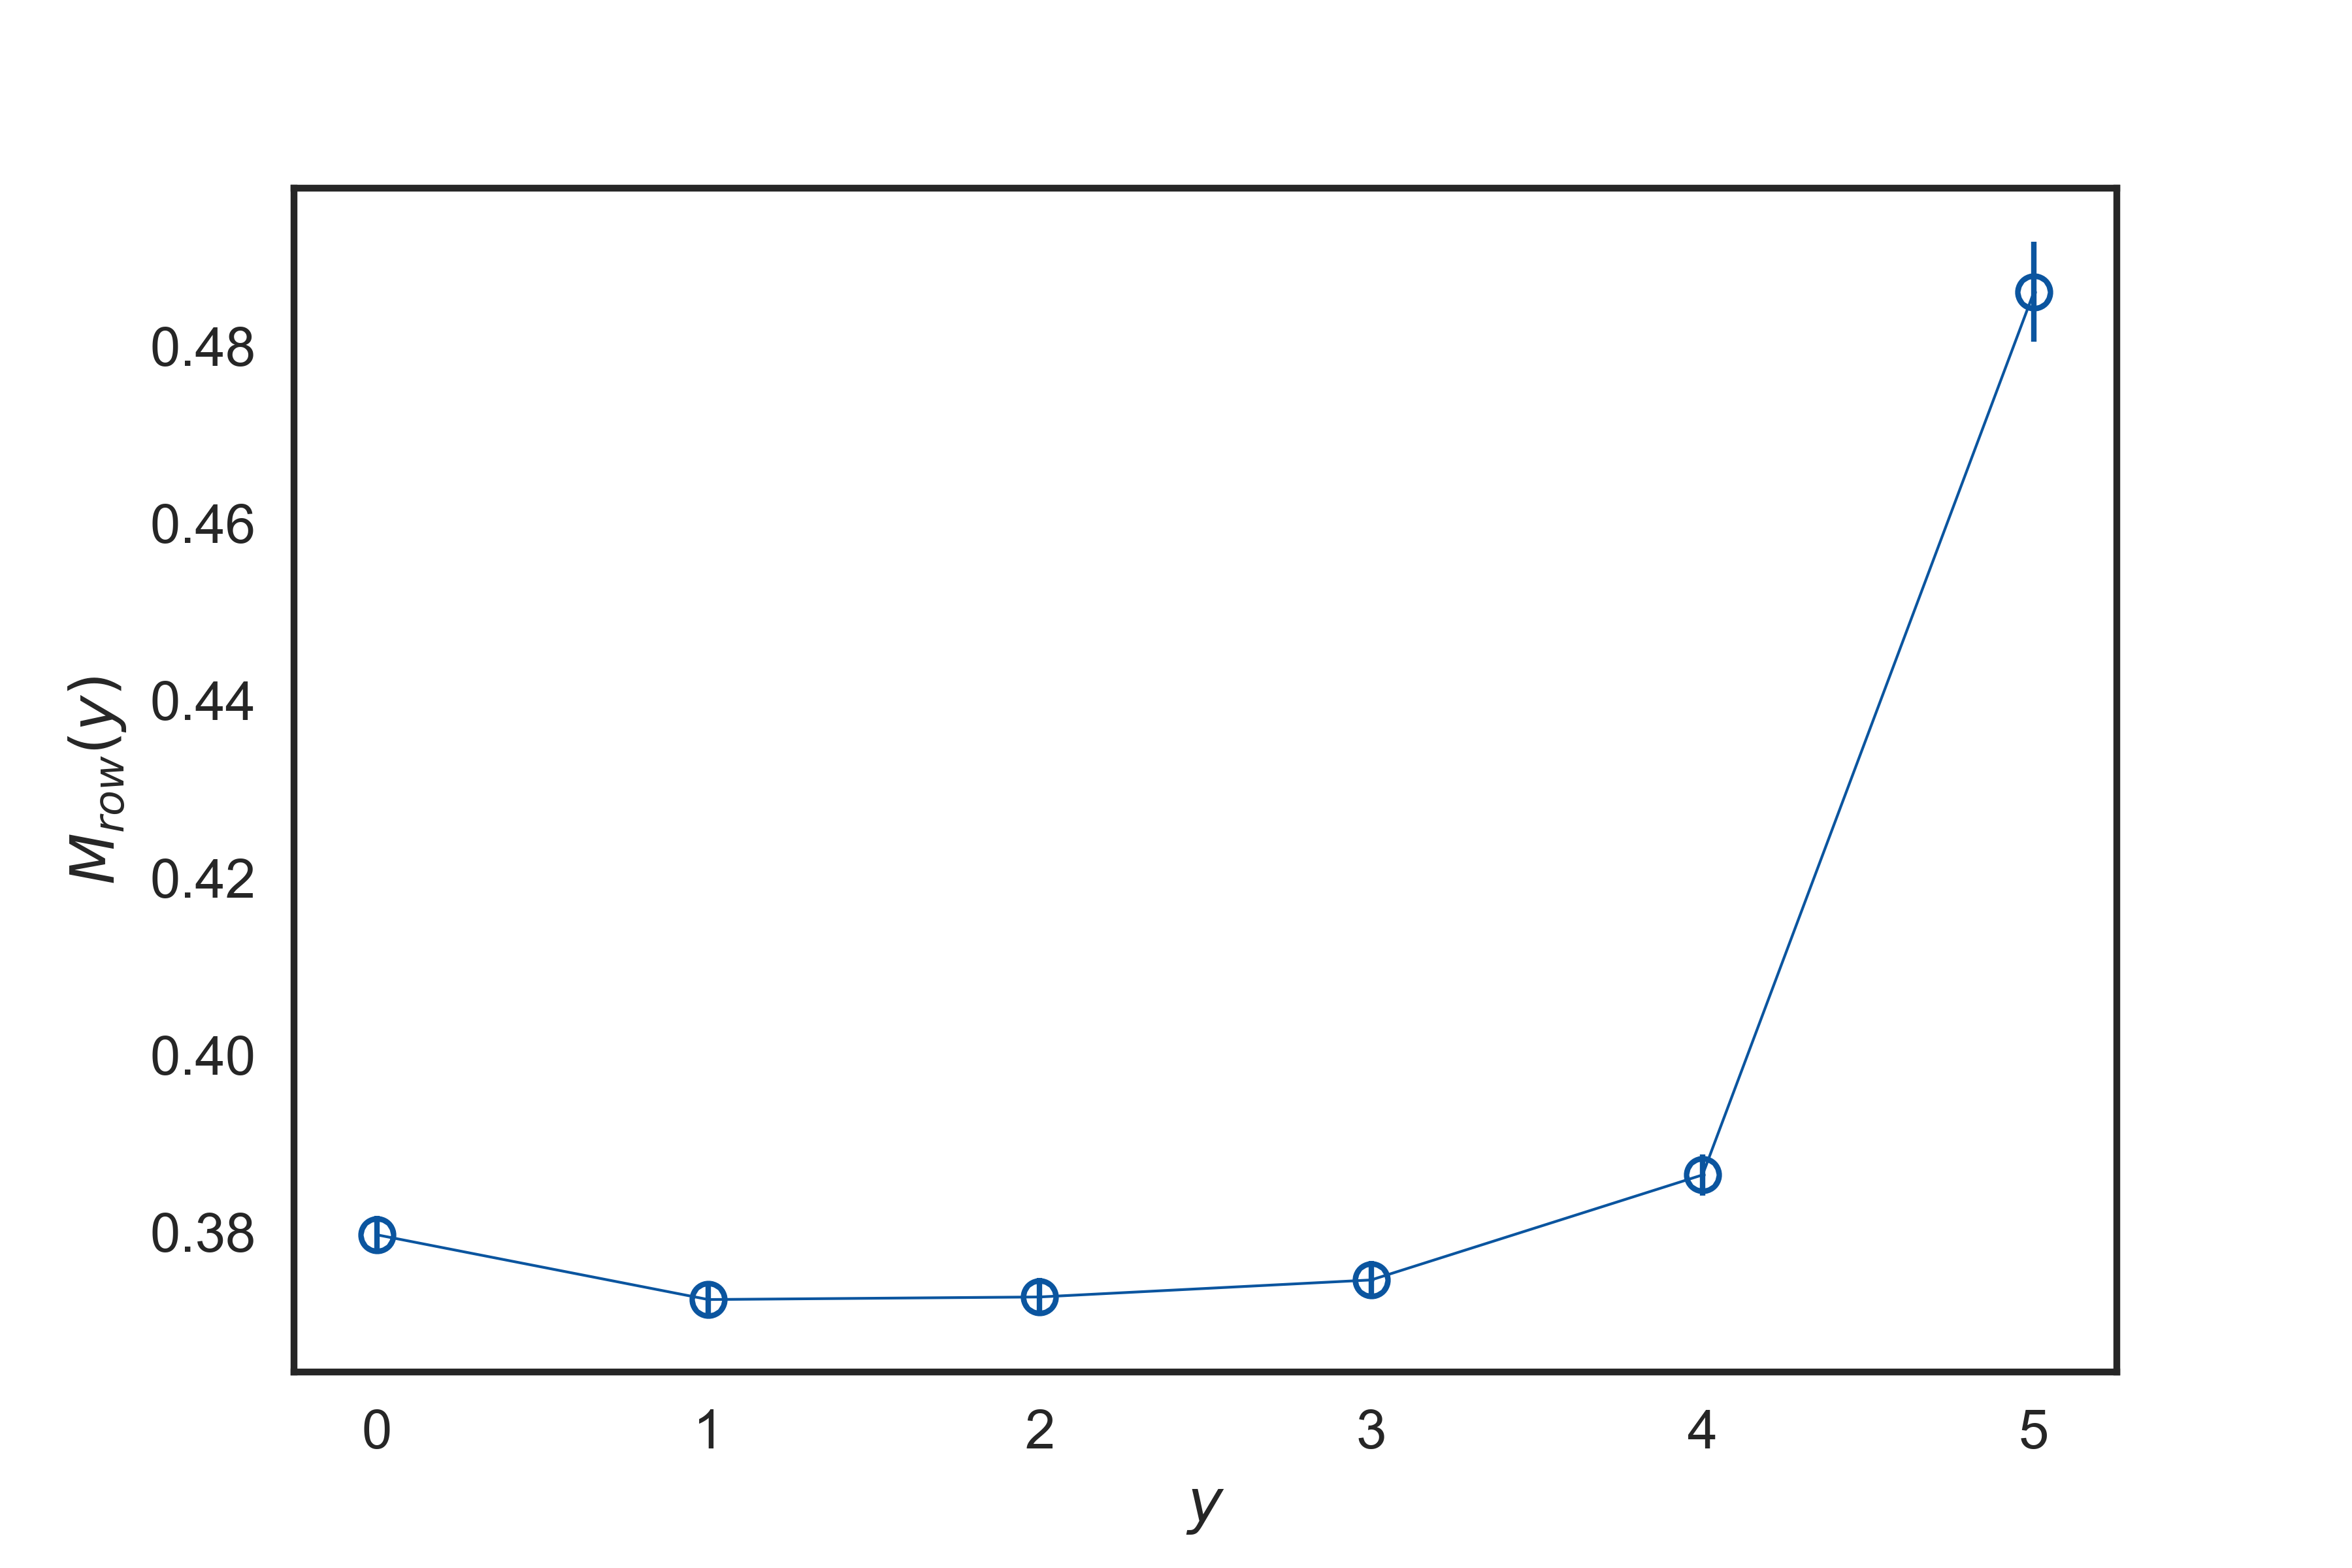
\includegraphics[scale = 0.55]{Applications/graphene-strain/order_parameter_Graphene.png}
	\caption[]{}
	\label{fig:edgeStFactor}
\end{figure}
\begin{figure}[H]
\hspace{-0.2cm}
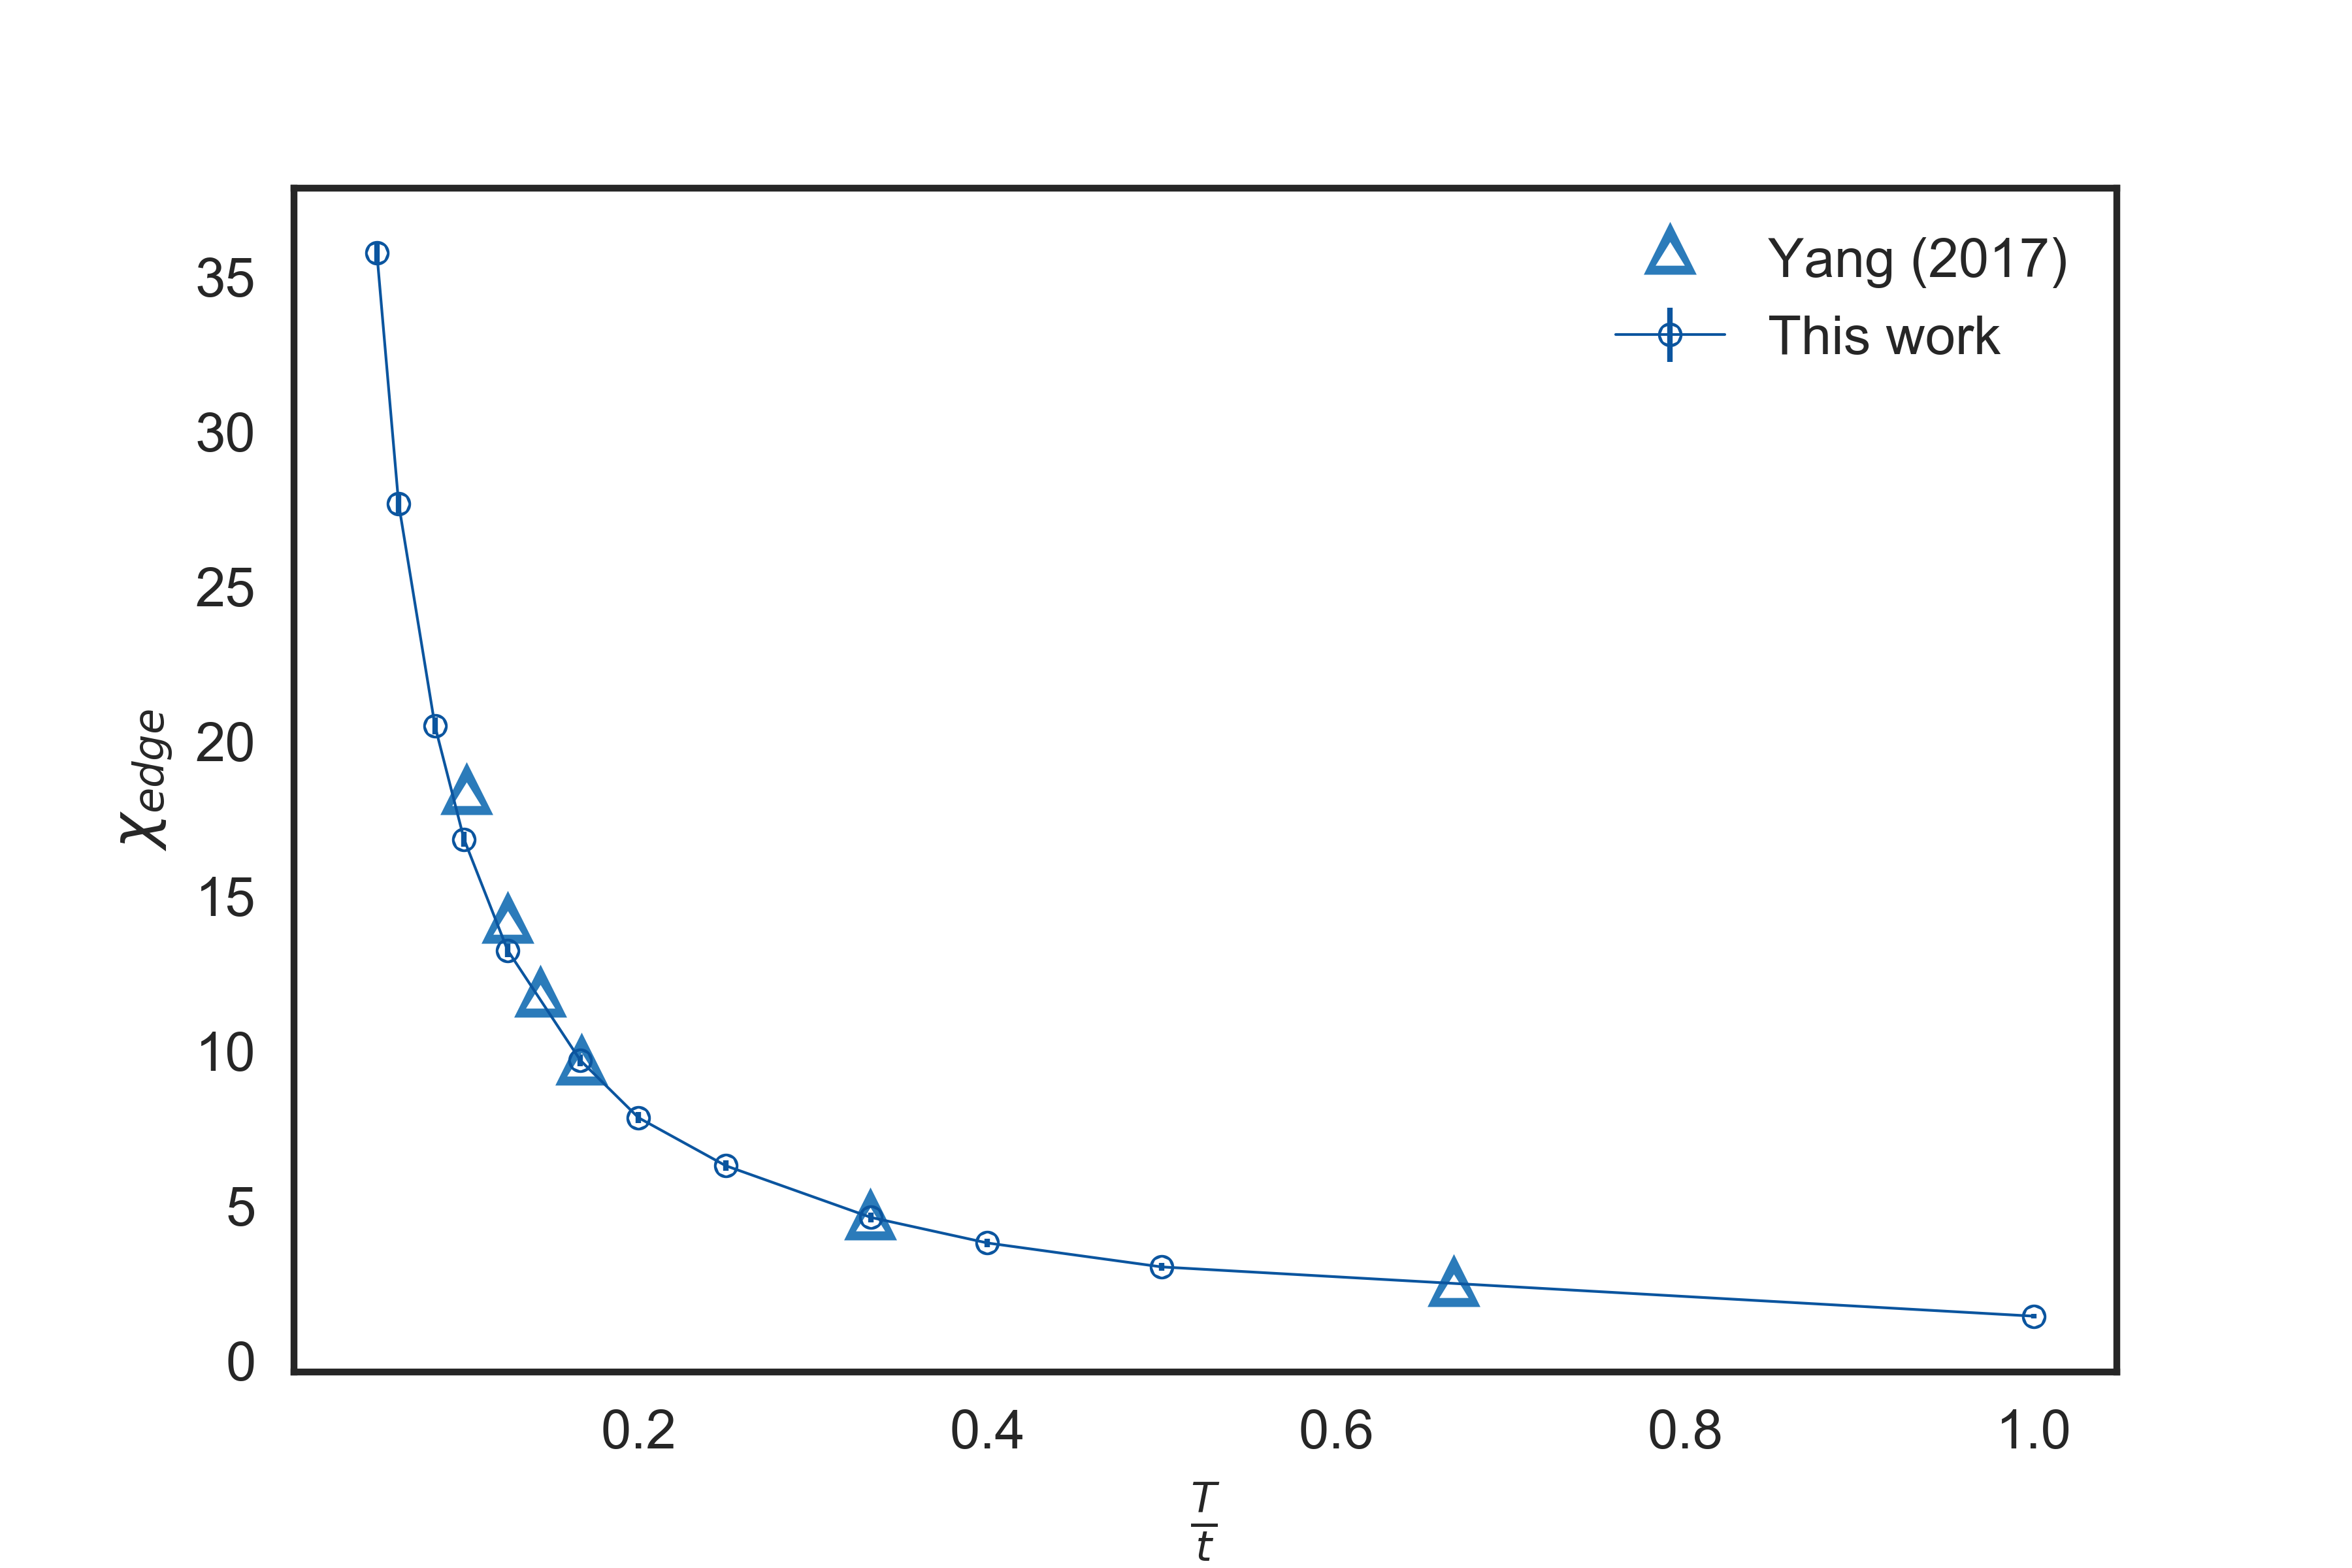
\includegraphics[scale = 0.55]{Applications/graphene-strain/chiTyang2017.png}
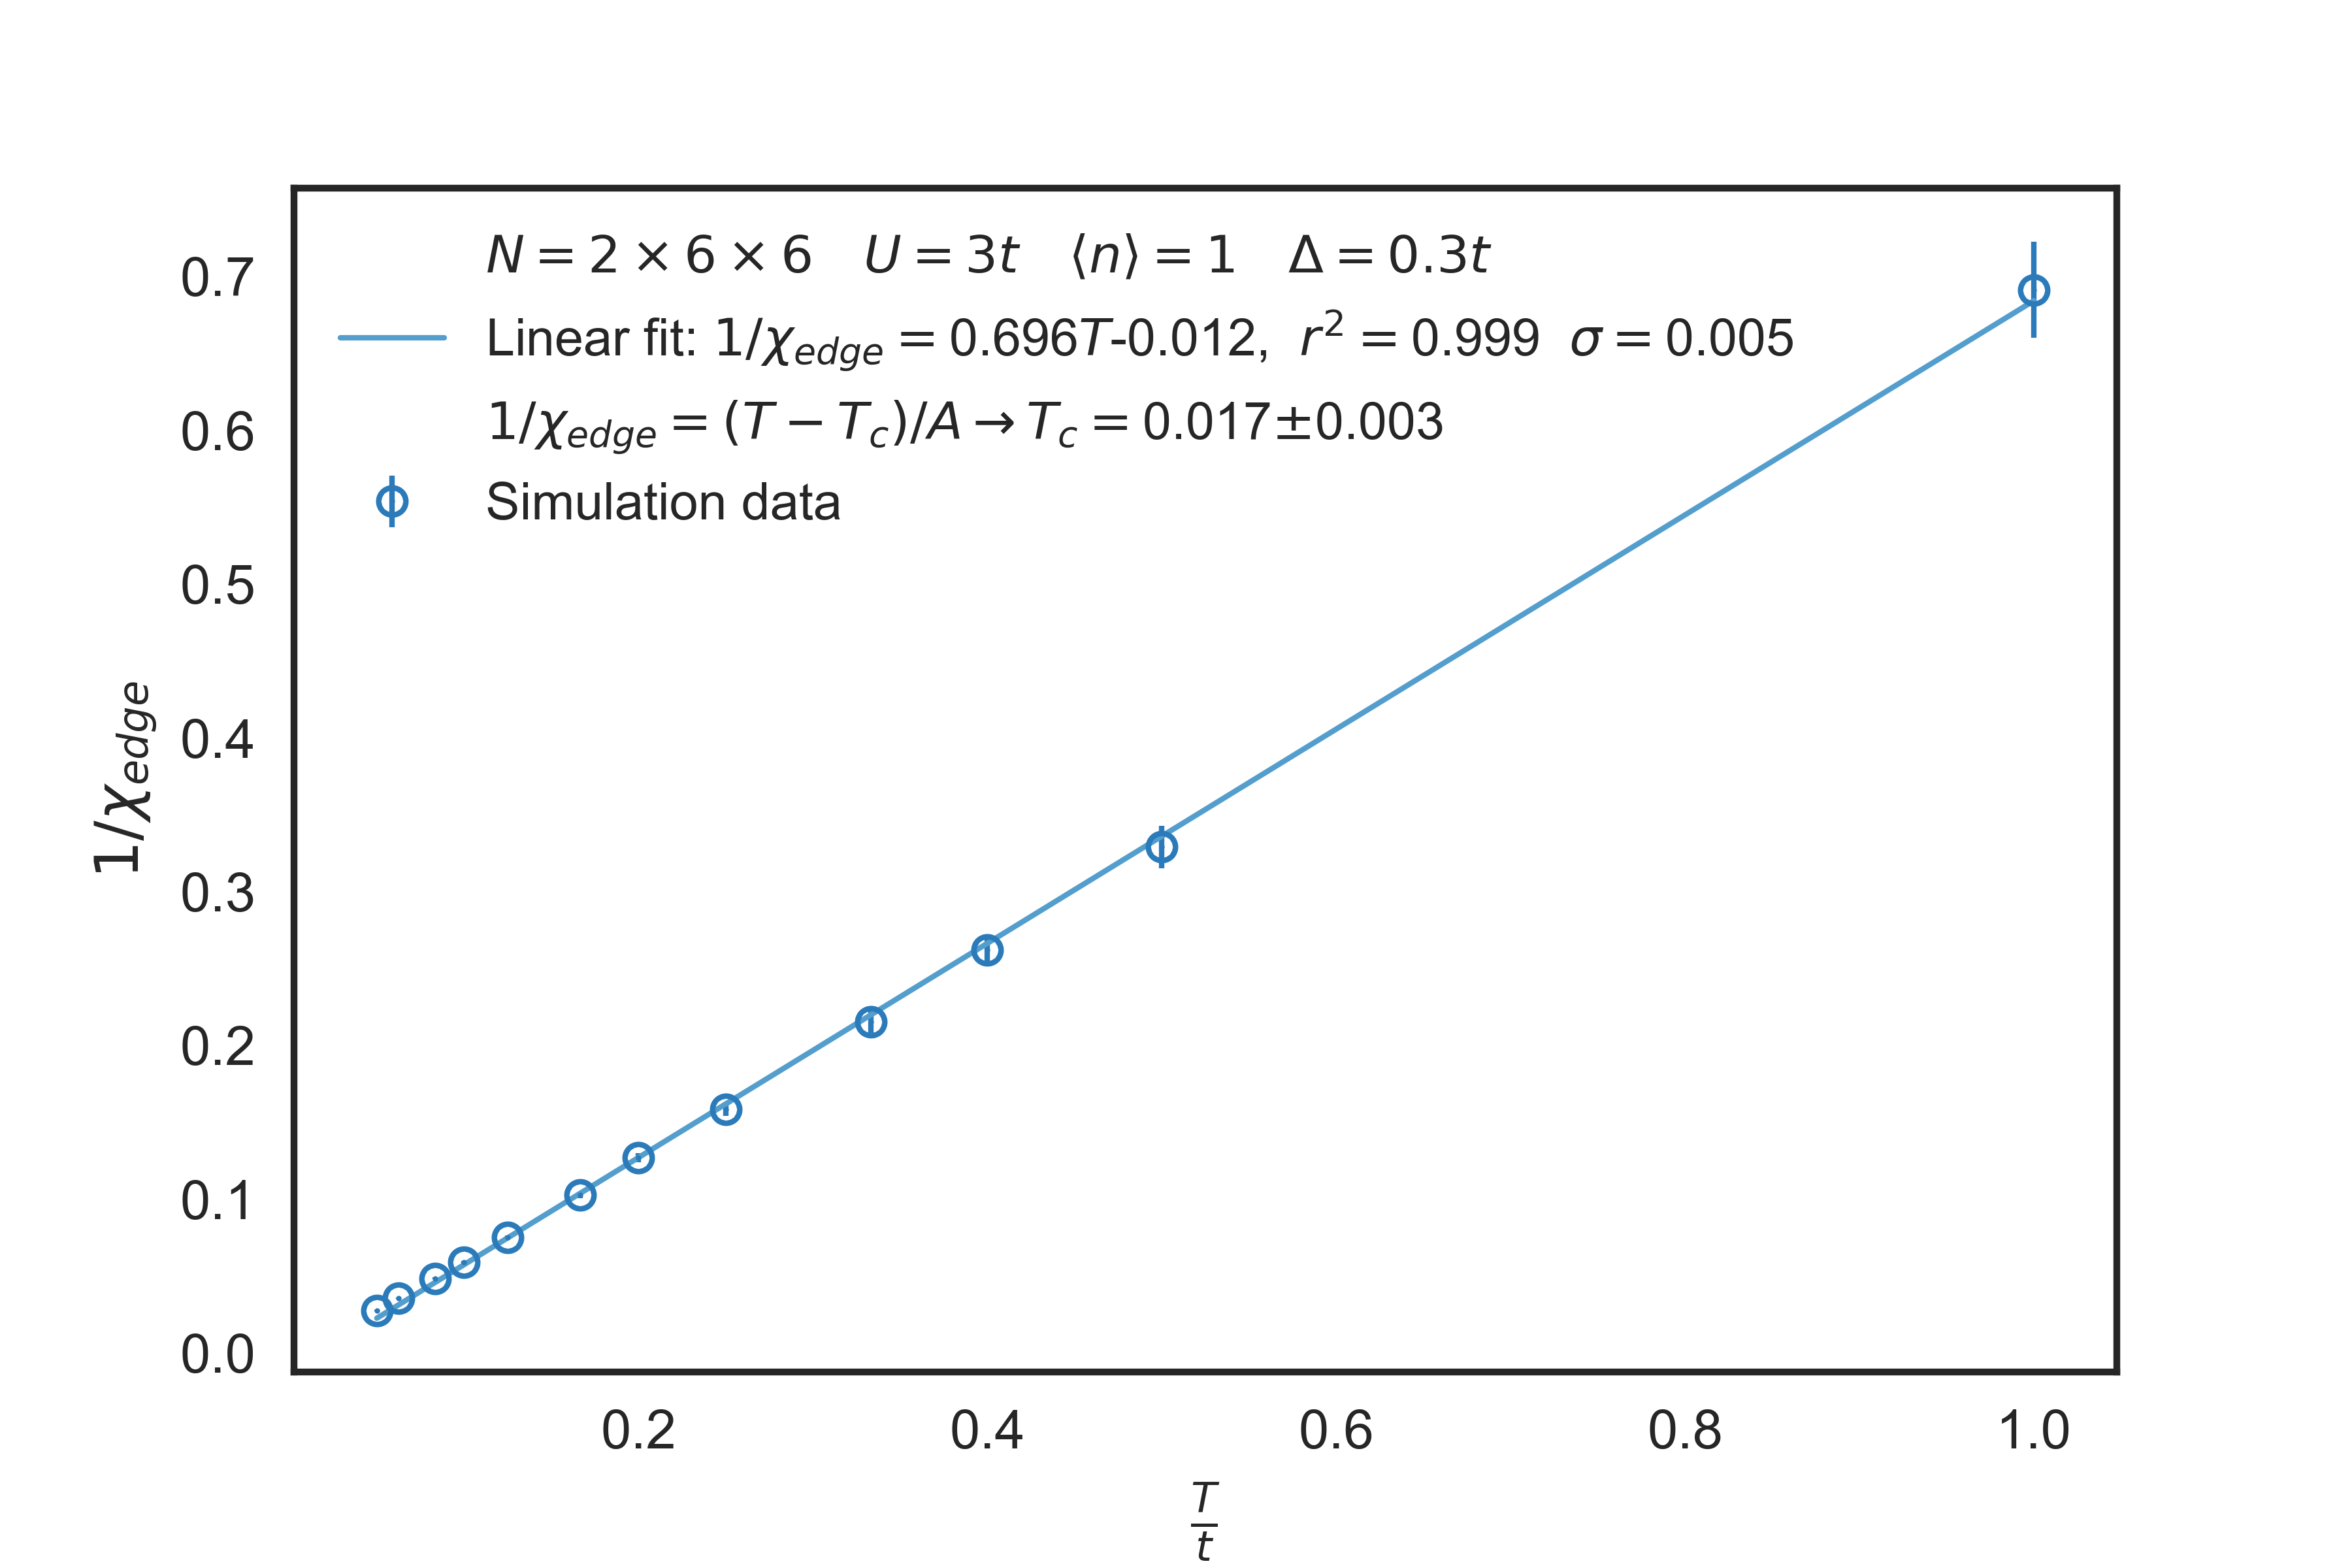
\includegraphics[scale = 0.55]{Applications/graphene-strain/fityang2017.png}
	\caption[]{}
	\label{fig:edgeStFactor}
\end{figure}

\subsection{\acp{TMD}}
\label{subsec:apTMD}

We start by approaching the \acs{TMDNR} problem at the mean field level.
Such a procedure is very useful to obtain a physical picture of the system's behavior.
In particular, at a given temperature, if there is a transition between a configuration with magnetic order, and a disordered one, there is a critical interaction parameter $U = U_c$ at which the transition occurs, and it can be estimated in mean field, and compared with the more precise, unbiased \acs{QMC} result.
In general, our mean field formulation would involve diagonalizing an $N \times N$ matrix at each step, where $N = N_{\text{orb}} N_x N_y$ is the size of the system times the number of orbitals.
However, since we consider \acs{PBC}s along the $x$-direction, we can partially diagonalize  the Hamiltonian analytically, reducing the size of the matrix to be diagonalized to $N_{\text{orb}} N_y \times N_{\text{orb}} N_y$, where $N_y$ is the width of the ribbon, i.e. the number of $\text{M}\text{X}_2$ formula units.
Consider the spinless 3-band tight binding model, with the lattice constant: $a \equiv 1$.
\begin{equation}
\begin{split}
\mathcal{H}_0 &= \sum_{\substack{m, n \\ \alpha, \beta}} \bigg( c_{m,n, \alpha}^\dagger t_{\alpha\beta}^0 c_{m, n, \beta} + \delta_{0, N_x}  c_{m,n, \alpha}^\dagger t_{\alpha\beta}^1 c_{m+1, n, \beta} + \delta_{-\sqrt{3}/2, (N_y -1)\sqrt{3}/2}  c_{m,n, \alpha}^\dagger t_{\alpha\beta}^4 c_{m-1, n, \beta} \\
& + \delta_{0, N_m} \delta_{-1, (N_y -1)\sqrt{3}/2} c_{m+1/2,n-\sqrt{3}/2, \alpha}^\dagger t_{\alpha\beta}^2 c_{m, n, \beta} + \delta_{-1, (N_y -1)\sqrt{3}/2} c_{m-1/2,n-\sqrt{3}/2, \alpha}^\dagger t_{\alpha\beta}^3 c_{m, n, \beta} \\
& + \delta_{N_y\sqrt{3}/2, 0} c_{m+1/2,n+\sqrt{3}/2, \alpha}^\dagger t_{\alpha\beta}^6 c_{m, n, \beta} + \delta_{-1, N_x -1} \delta_{N_y\sqrt{3}/2, 0} c_{m-1/2,n+\sqrt{3}/2, \alpha}^\dagger t_{\alpha\beta}^5 c_{m, n, \beta} \bigg)
\end{split}
\end{equation}

Fourier transforming along $m$: $c_{m, n, \alpha} = \frac{1}{\sqrt{N_x}}\sum_{k} e^{-i k m } c_{k, n, \alpha} $, with $k = \frac{2\pi}{N_x} \{ -\frac{N_x}{2} + 1, -\frac{N_x}{2}, ..., \frac{N_x}{2} \}$:
\begin{equation}
\begin{split}
\mathcal{H}_0 &= \sum_{ \substack{k, y \\ \alpha, \beta} } \bigg( c_{k, y, \alpha}^\dagger (t_{\alpha \beta}^0  + e^{ik} t_{\alpha \beta}^1 + e^{-ik} t_{\alpha \beta}^4 )  c_{k, y, \beta} + \delta_{-1, N_y -1} c_{k, y - 1, \alpha}^\dagger ( e^{ik/2} t_{\alpha \beta}^2 + e^{-ik/2} t_{\alpha \beta}^3 ) c_{k, y, \beta} \\
& + \delta_{N_y, 0} c_{k, y, \alpha}^\dagger ( e^{ik/2} t_{\alpha \beta}^6 + e^{-ik/2} t_{\alpha \beta}^5 ) c_{k, y+1, \beta} \bigg) , \,\, \text{with} \, y \, \text{defined as in Fig.(4.1)}
\end{split}
\end{equation}
leading to a tridiagonal block $3 N_y \times 3 N_y$ hopping matrix $\bm H (k)$ with three different types of matrix elements: $\bm h_1 = \bm H_{y,y}$, $\bm h_2 = \bm H_{y,y-1}$, $\bm h_2^\dagger = \bm H_{y, y+1}$.
\begin{equation}
[ H_{(\alpha y) (\beta y')} (k) ] = 
\begin{pmatrix}
\bm h_1 & \bm h_2^\dagger & & & \\
\bm h_2 & \bm h_1 & \bm h_2^\dagger & & \\
& \bm h_2 & \bm h_1 & \ddots & \\
& & \ddots & \ddots & \bm h_2^\dagger \\
& & & \bm h_2 & \bm h_1
\end{pmatrix}, \, 
\bm h_1 = 
\begin{pmatrix}
\varepsilon_1 + 2 t_0 \cos k & 2 i t_1 \sin k & 2 t_2 \cos k \\
-2 i t_1 \sin k & \varepsilon_2 + 2 t_{11} \cos k & 2 i t_{12} \sin k \\
2 t_2 \cos k& -2 i t_{12} \sin k & \varepsilon_2 + 2 t_{22} \cos k \\
\end{pmatrix}
\end{equation}
\begin{equation*}
\bm h_2 =
\begin{pmatrix}
2 t_0 \cos ( k / 2 ) & i \sin ( k / 2 ) \bigg( t_1 - \sqrt{3} t_2 \bigg) & - \cos (k /2 ) \bigg( \sqrt{3} t_1 + t_2 \bigg) \\
-i \sin ( k / 2 ) \bigg(t_1 + \sqrt{3} t_2 \bigg) & \frac{1}{2} \cos (k / 2) \bigg( t_{11} + 3 t_{22} \bigg) & -i \sin (k / 2) \bigg( \frac{\sqrt{3}}{2} (t_{11} -  t_{22} ) + 2 t_{12} \bigg) \\
\cos ( k / 2) \bigg( \sqrt{3} t_1 - t_2 \bigg) & -i \sin (k / 2) \bigg( \frac{\sqrt{3}}{2} ( t_{11} - t_{22} ) - 2 t_{12} \bigg) & \frac{1}{2} \cos (k / 2) \bigg( 3 t_{11	} + t_{22} \bigg)
\end{pmatrix}
\end{equation*}
\begin{figure}[H]
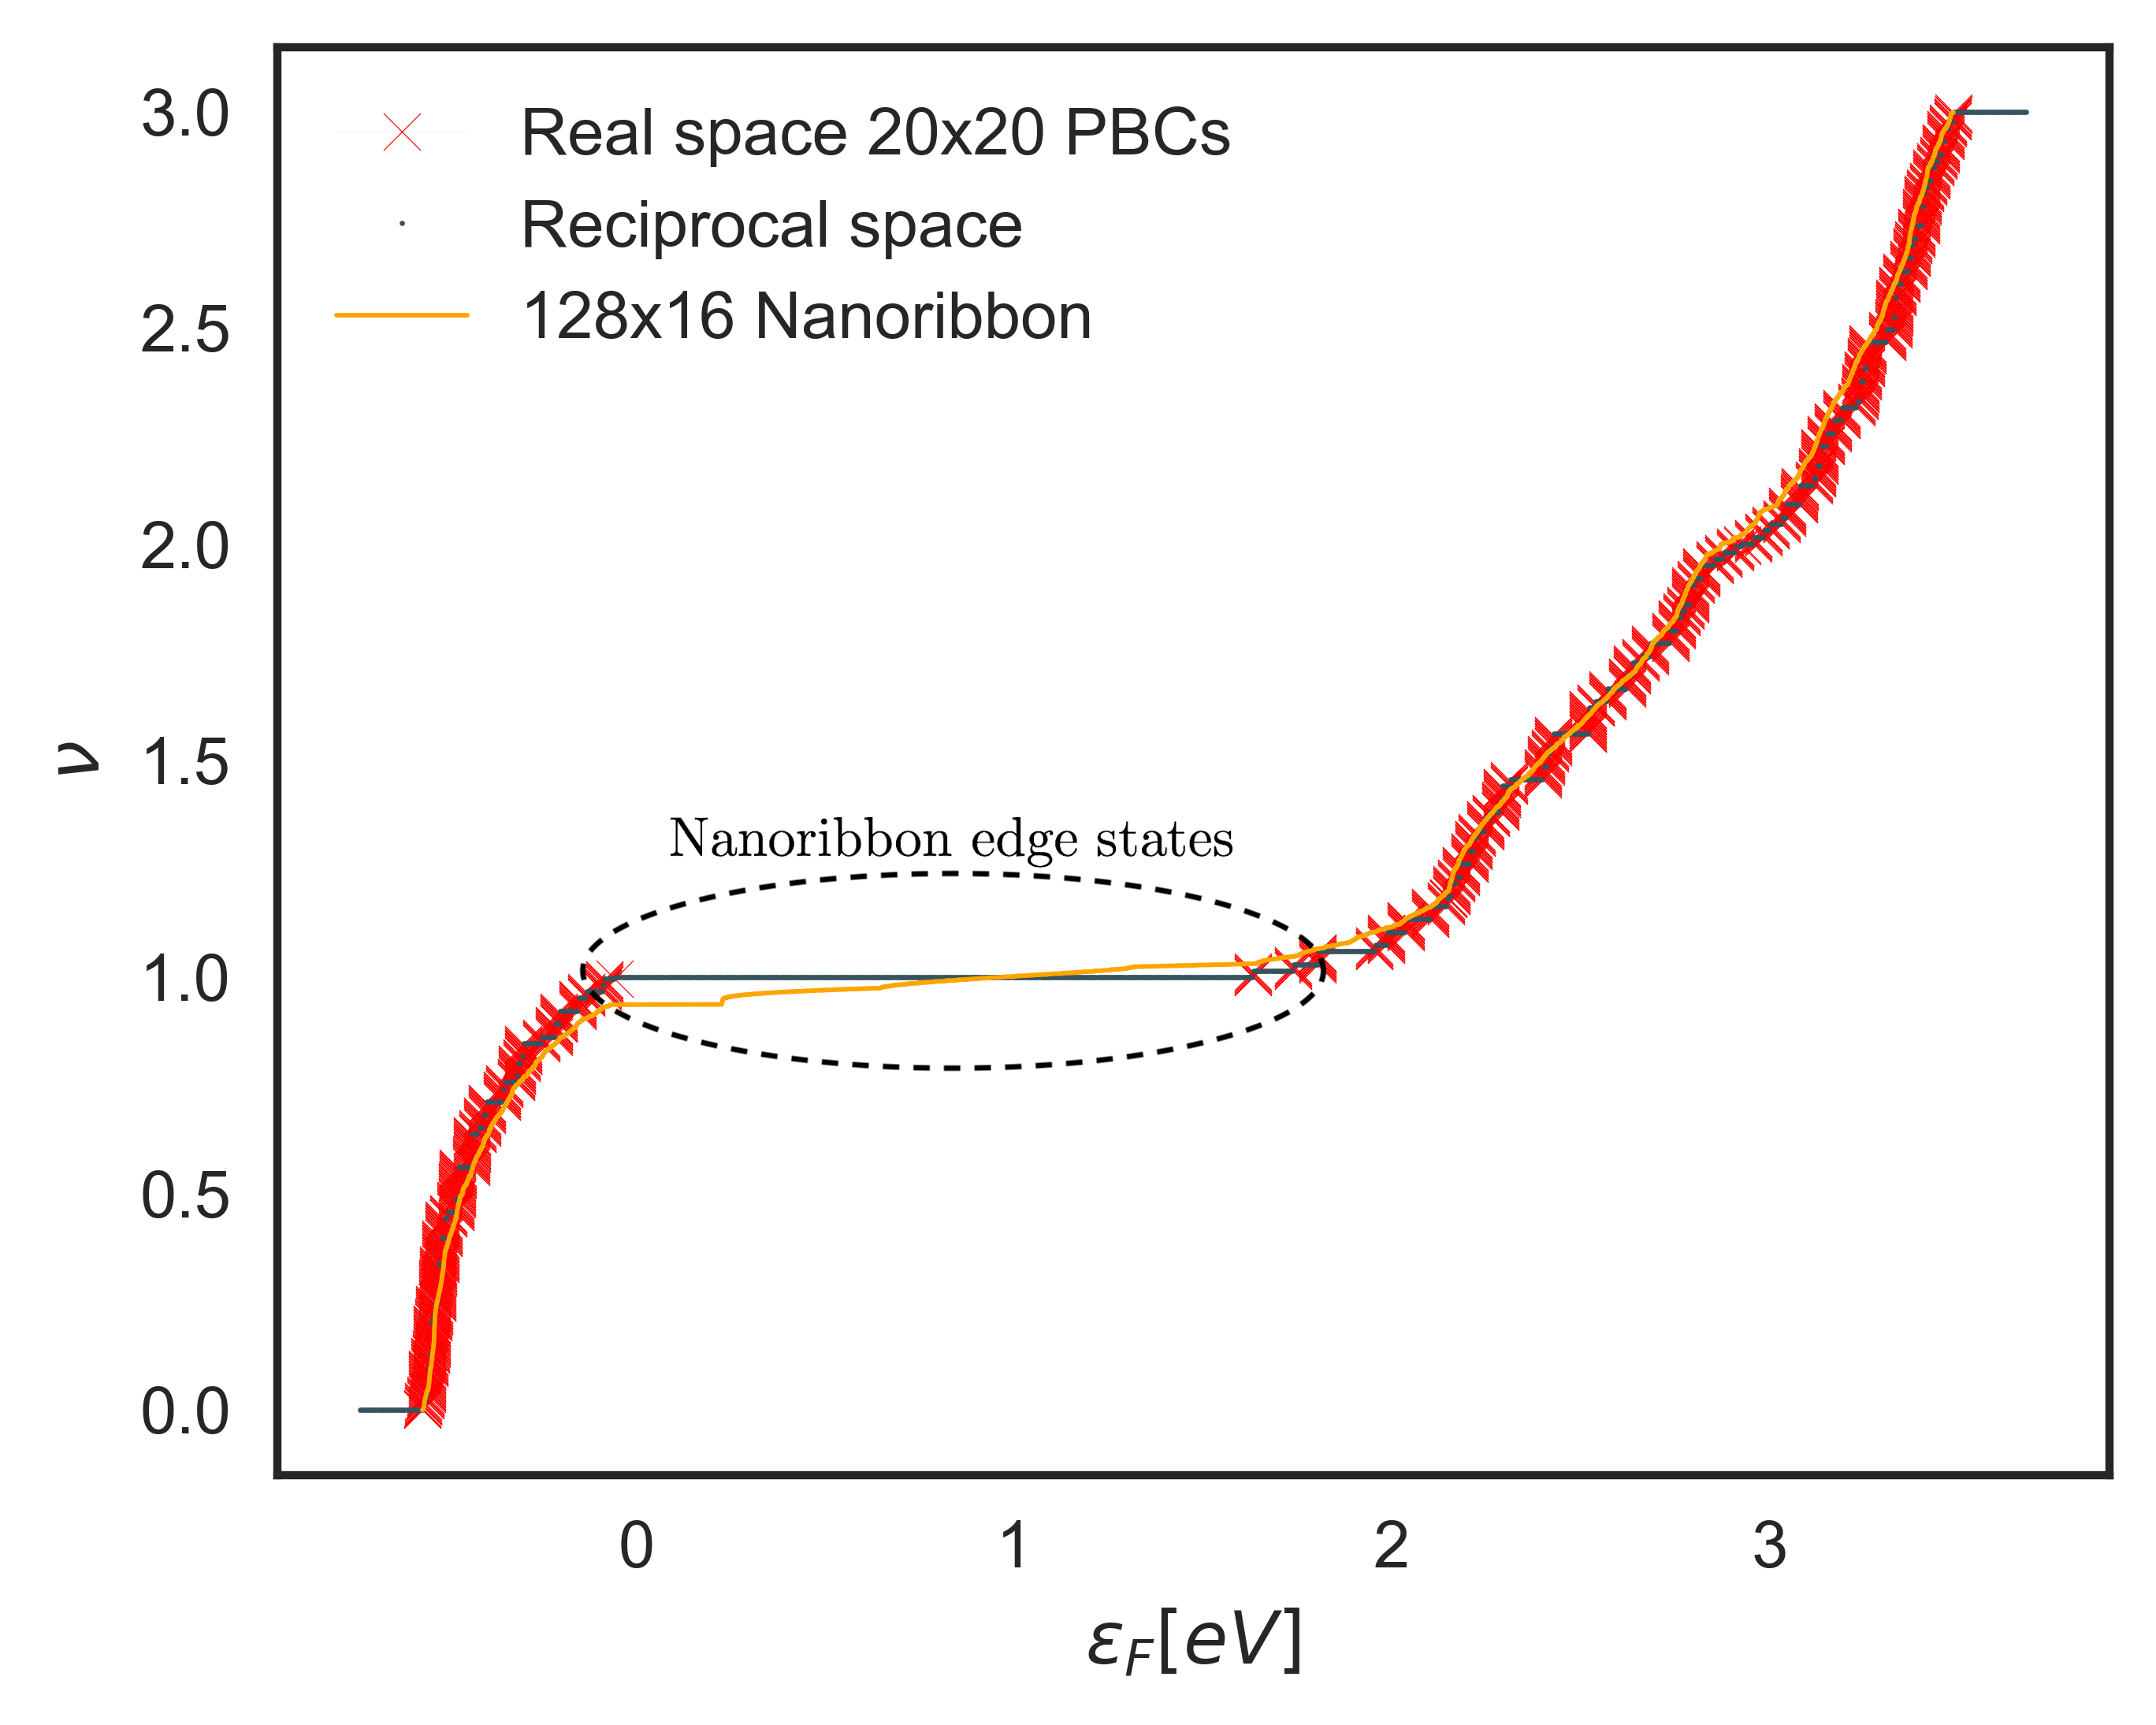
\includegraphics[scale=0.55]{Applications/fillingVsE.png}
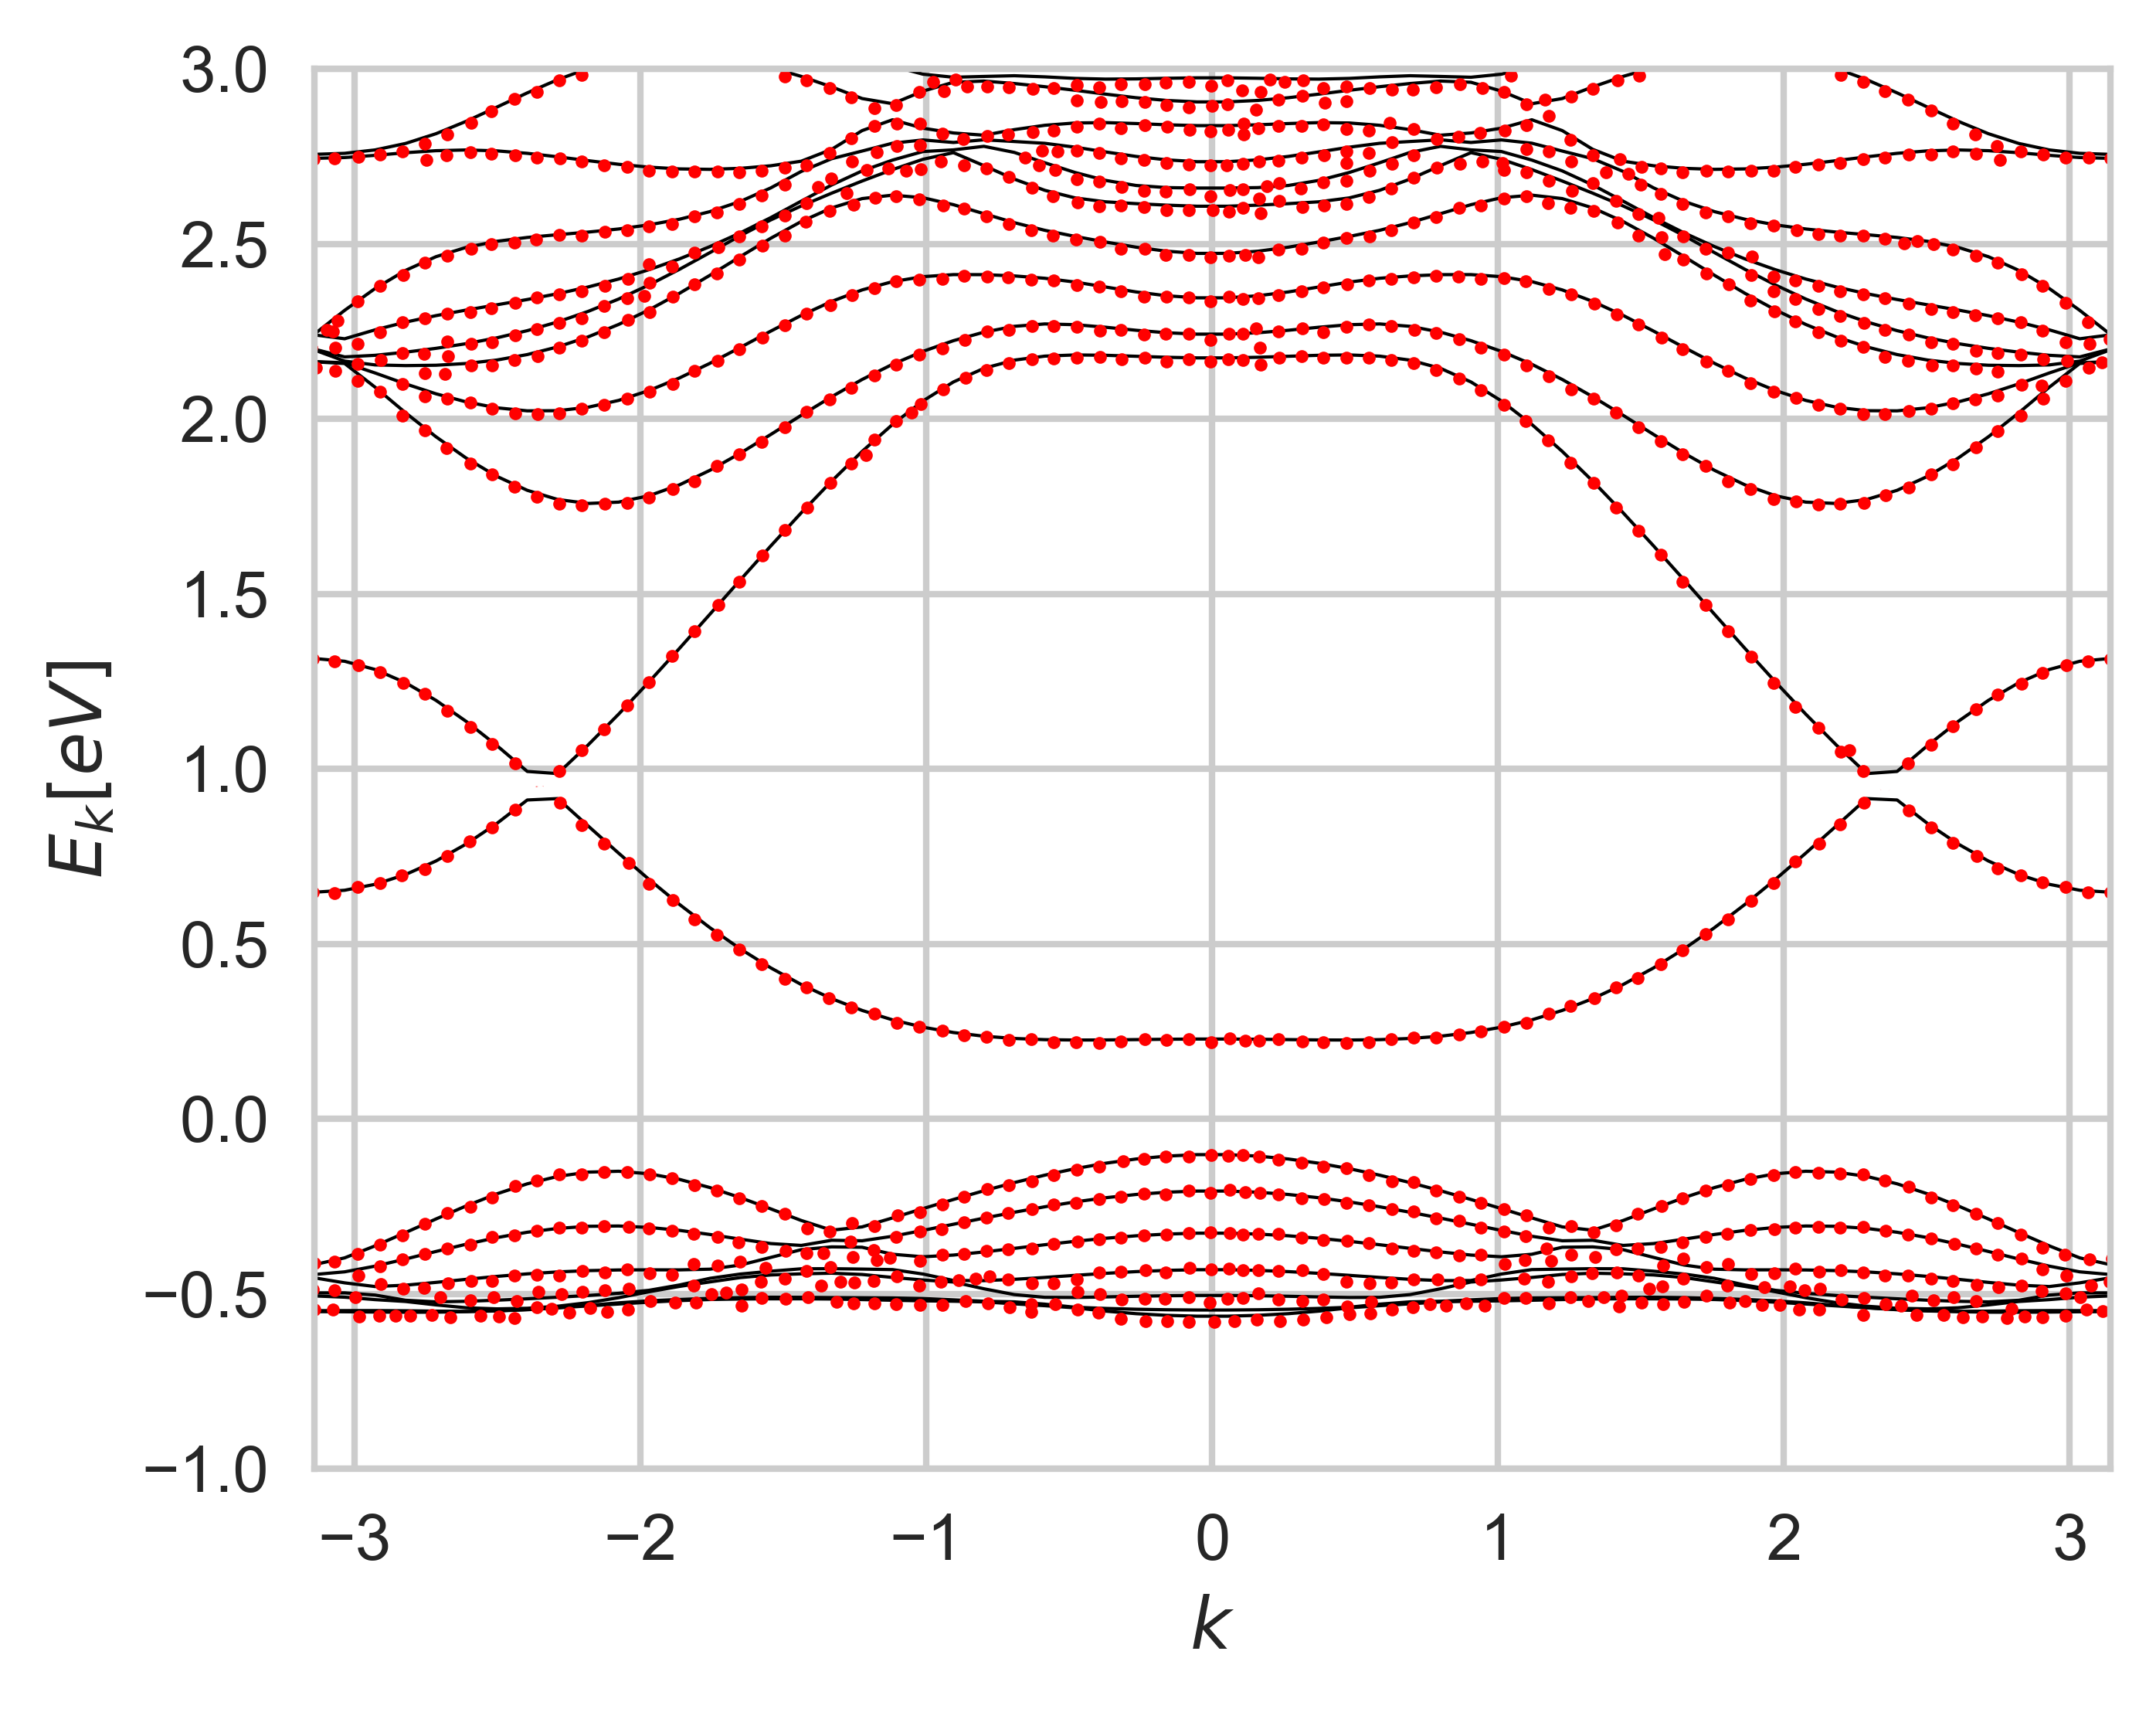
\includegraphics[scale=0.55]{Applications/BandStructureNanoribbonTMD.png}
	\caption[Filling $\nu$ as a function of the Fermi energy $\varepsilon_F$ for a \acs{TMD} monolayer and a nanoribbon. $\text{Mo}\text{S}_2$.  \acs{TMDNR} band structure obtained by the 3-band model.]{Left: Filling $\nu$ as a function of the Fermi energy $\varepsilon_F$ for a system with \acp{PBC}, as computed by diagonalizing the input matrix of our code, and by the hopping matrix in $\bm k$-space. Comparison between the fillings of a nanoribbon and a periodic system.
	For the nanoribbon, edge states appear on the gap of the periodic system.
	Right: 3-band model $\text{Mo}\text{S}_2$ zigzag edged nanoribbon energy bands (red dots and orange curve), for $N_y = 8$, using the GCA parameters. The first principles bands show the contribution from orbitals that are not considered in the 3-band model (blue:  $d_{z^2}$, $d_{xy}$, $d_{x^2-y^2}$, green: others). The 3-band model reproduces the bands that correspond to the orbitals taken into account reasonably (1 and 2 correspond to the edge states from the $d_{z^2}$, $d_{xy}$, $d_{x^2-y^2}$ orbitals of the $\text{Mo}$ atoms, while 3 and 4 correspond to the $d_{yz}$ orbital at the $\text{Mo}$-terminated edge, and $p_{y, z}$ orbitals from the $\text{S}$-terminated edge, and are not taken into account in the 3-band model).\cite{liu_three-band_2013}.}
	\label{fig:fillingVsE}
\end{figure}

By applying our mean field approach to solve the 3-band model with Hubbard-type interactions, we obtain solutions that are independent of $x$, which motivates us to reduce the number of MF parameters by choosing a translationally invariant ansatz.
This is equivalent to taking $\left\langle n_{x, y,\alpha, \sigma}\right\rangle = \left\langle n_{y,\alpha, \sigma}\right\rangle  \forall x$ ($6 N_y$ parameters).
By reducing the number of parameters, convergence is facilitated, which allows us to evaluate whether the solution of Fig.(\ref{fig:nanoGraphVsTMD}) is robust, i.e. whether it corresponds to a metastable or not.
The mean field form of the interaction term with the reduced number of parameters changes, implying that the self-consistent relation of Eq.(\ref{eq:selfConsistent}) from which the local densities are computed changes as well.
\begin{equation}
\mathcal{H}_{\text{MF}} = \mathcal{H}_0 + \mathcal{H}_1 + \mathcal{C} , \,\text{where} \,\, \mathcal{H}_1 = U \sum_{m, n, \alpha}  \sum_\sigma n_{\substack{m, \sigma \\ n, \alpha}} \big\langle n_{\substack{m, -\sigma \\ n, \alpha}} \big\rangle  , \,\, \mathcal{C} = -U  \sum_{m, n, \alpha} \big\langle n_{\substack{m, \uparrow \\ n, \alpha}} \big\rangle \big\langle n_{\substack{m, \downarrow \\ n, \alpha}} \big\rangle
\end{equation}
\begin{equation}
\begin{split}
\mathcal{H}_1 + \mathcal{C} &= \frac{U}{N_x^{\,2}} \sum_{\substack{n \alpha \\ k_1 k_2 \\ k_3 k_4}} \underbrace{\sum_m e^{i [ (k_1 + k_3) - (k_2 + k_4) ] m}}_{N_x \delta_{k_4, k_1 + k_3 - k_2}} \bigg( \sum_\sigma c_{\substack{k_1, \sigma \\ n, \alpha}}^\dagger c_{\substack{k_2, \sigma \\ n, \alpha}} \underbrace{\big\langle c_{\substack{k_3, -\sigma\\ n, \alpha}}^\dagger c_{\substack{k_4, -\sigma \\ n, \alpha}} \big\rangle}_{\delta_{k_3, k_4} \big\langle n_{\substack{k_3,-\sigma \\ n, \alpha}} \big\rangle} - \underbrace{\big\langle c_{\substack{k_1, \uparrow \\ n, \alpha}}^\dagger c_{\substack{k_2  \uparrow \\n, \alpha}} \big\rangle}_{\delta_{k_1, k_2} \big\langle n_{\substack{k_2,\uparrow \\ n, \alpha}} \big\rangle} \underbrace{\big\langle c_{\substack{k_3, \downarrow \\ n, \alpha}}^\dagger c_{\substack{k_4, \downarrow \\ n, \alpha}} \big\rangle}_{\delta_{k_3, k_4} \big\langle n_{\substack{k_3,\downarrow \\ n, \alpha}} \big\rangle}  \bigg) \\
&= \frac{U}{N_x} \sum_{\substack{n \alpha \\ k_2 k_3}} \bigg( \sum_\sigma n_{\substack{k_2, \sigma \\ n, \alpha}} \big\langle n_{\substack{k_3, -\sigma \\ n, \alpha}} \big\rangle - \big\langle n_{\substack{k_2, \uparrow \\ n, \alpha}} \big\rangle \big\langle n_{\substack{k_3, \downarrow \\ n, \alpha}} \big\rangle \bigg) \equiv
U \sum_{k, \mu} \bigg( \sum_\sigma n_{k,\mu, \sigma} \big\langle n_{\mu, -\sigma} \big\rangle - \big\langle n_{\mu, \uparrow} \big\rangle \big\langle n_{\mu, \downarrow} \big\rangle \bigg)
\end{split}
\end{equation}
where we collapsed the indexes $(n, \alpha)$ into a single index $\mu$.
The self consistent relation allowing us to compute the new MF parameters at each step emerges by diagonalizing $\mathcal{H}_1$ in the $\mu$-subspace:
\begin{equation}
\big\langle n_{\mu, \sigma} \big\rangle = \frac{1}{N_x}\sum_{q, \nu} | Q_{q \sigma \mu, \nu} |^2 \rho ( \varepsilon_{q \nu \sigma} ) , \, \text{where} \,\, d_{q, \sigma, \nu} = \sum_\nu Q_{q \sigma \mu, \nu}^\star c_{q ,\sigma, \mu} ,  \, \text{and} \,\, \mathcal{H}_{\text{MF}} = \sum_{q, \nu, \sigma} \varepsilon_{q, \nu, \sigma} d_{q, \nu, \sigma}^\dagger d_{q, \nu, \sigma} + \mathcal{C}
\end{equation}
\begin{figure}[H]
\hspace{0.1cm}
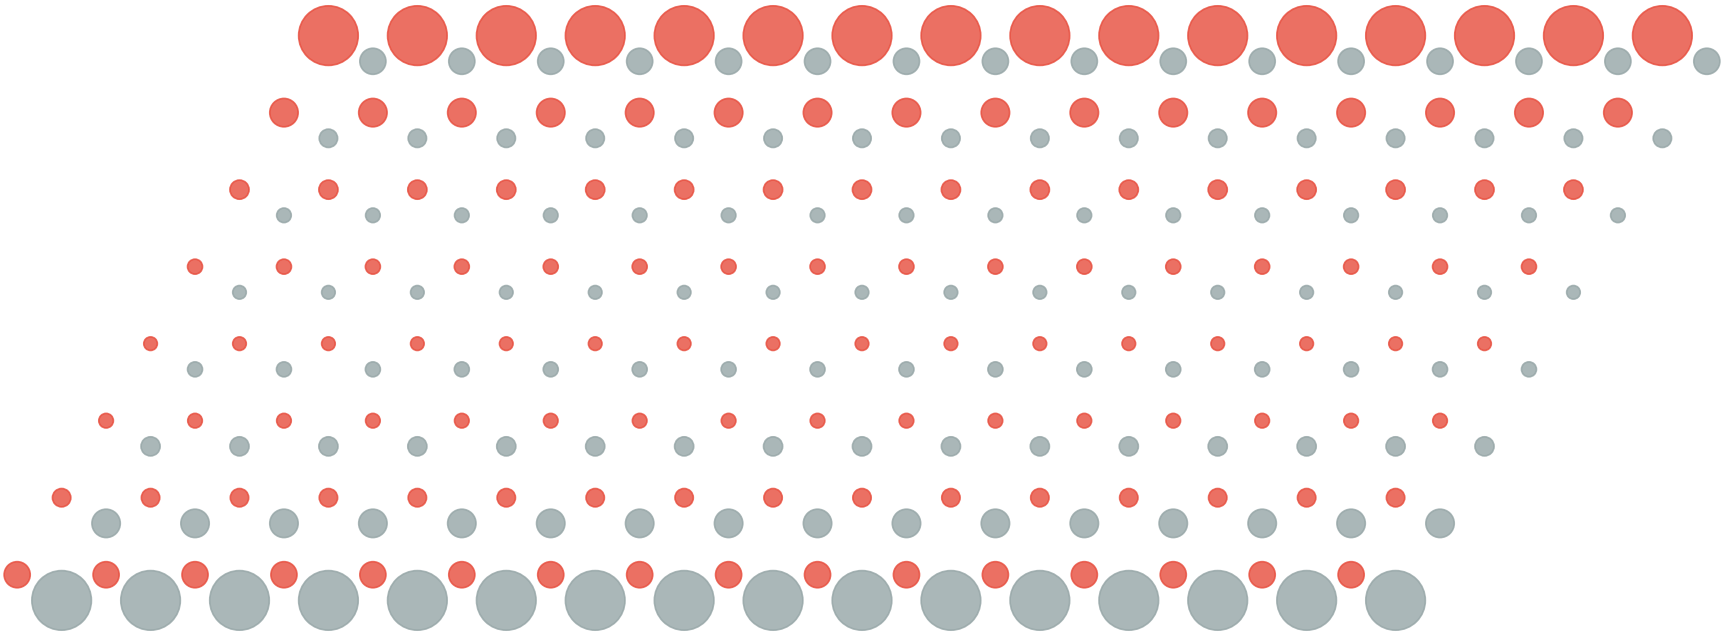
\includegraphics[scale=1.023]{Applications/MFnanoribbon.png}
\hspace{0.05cm}
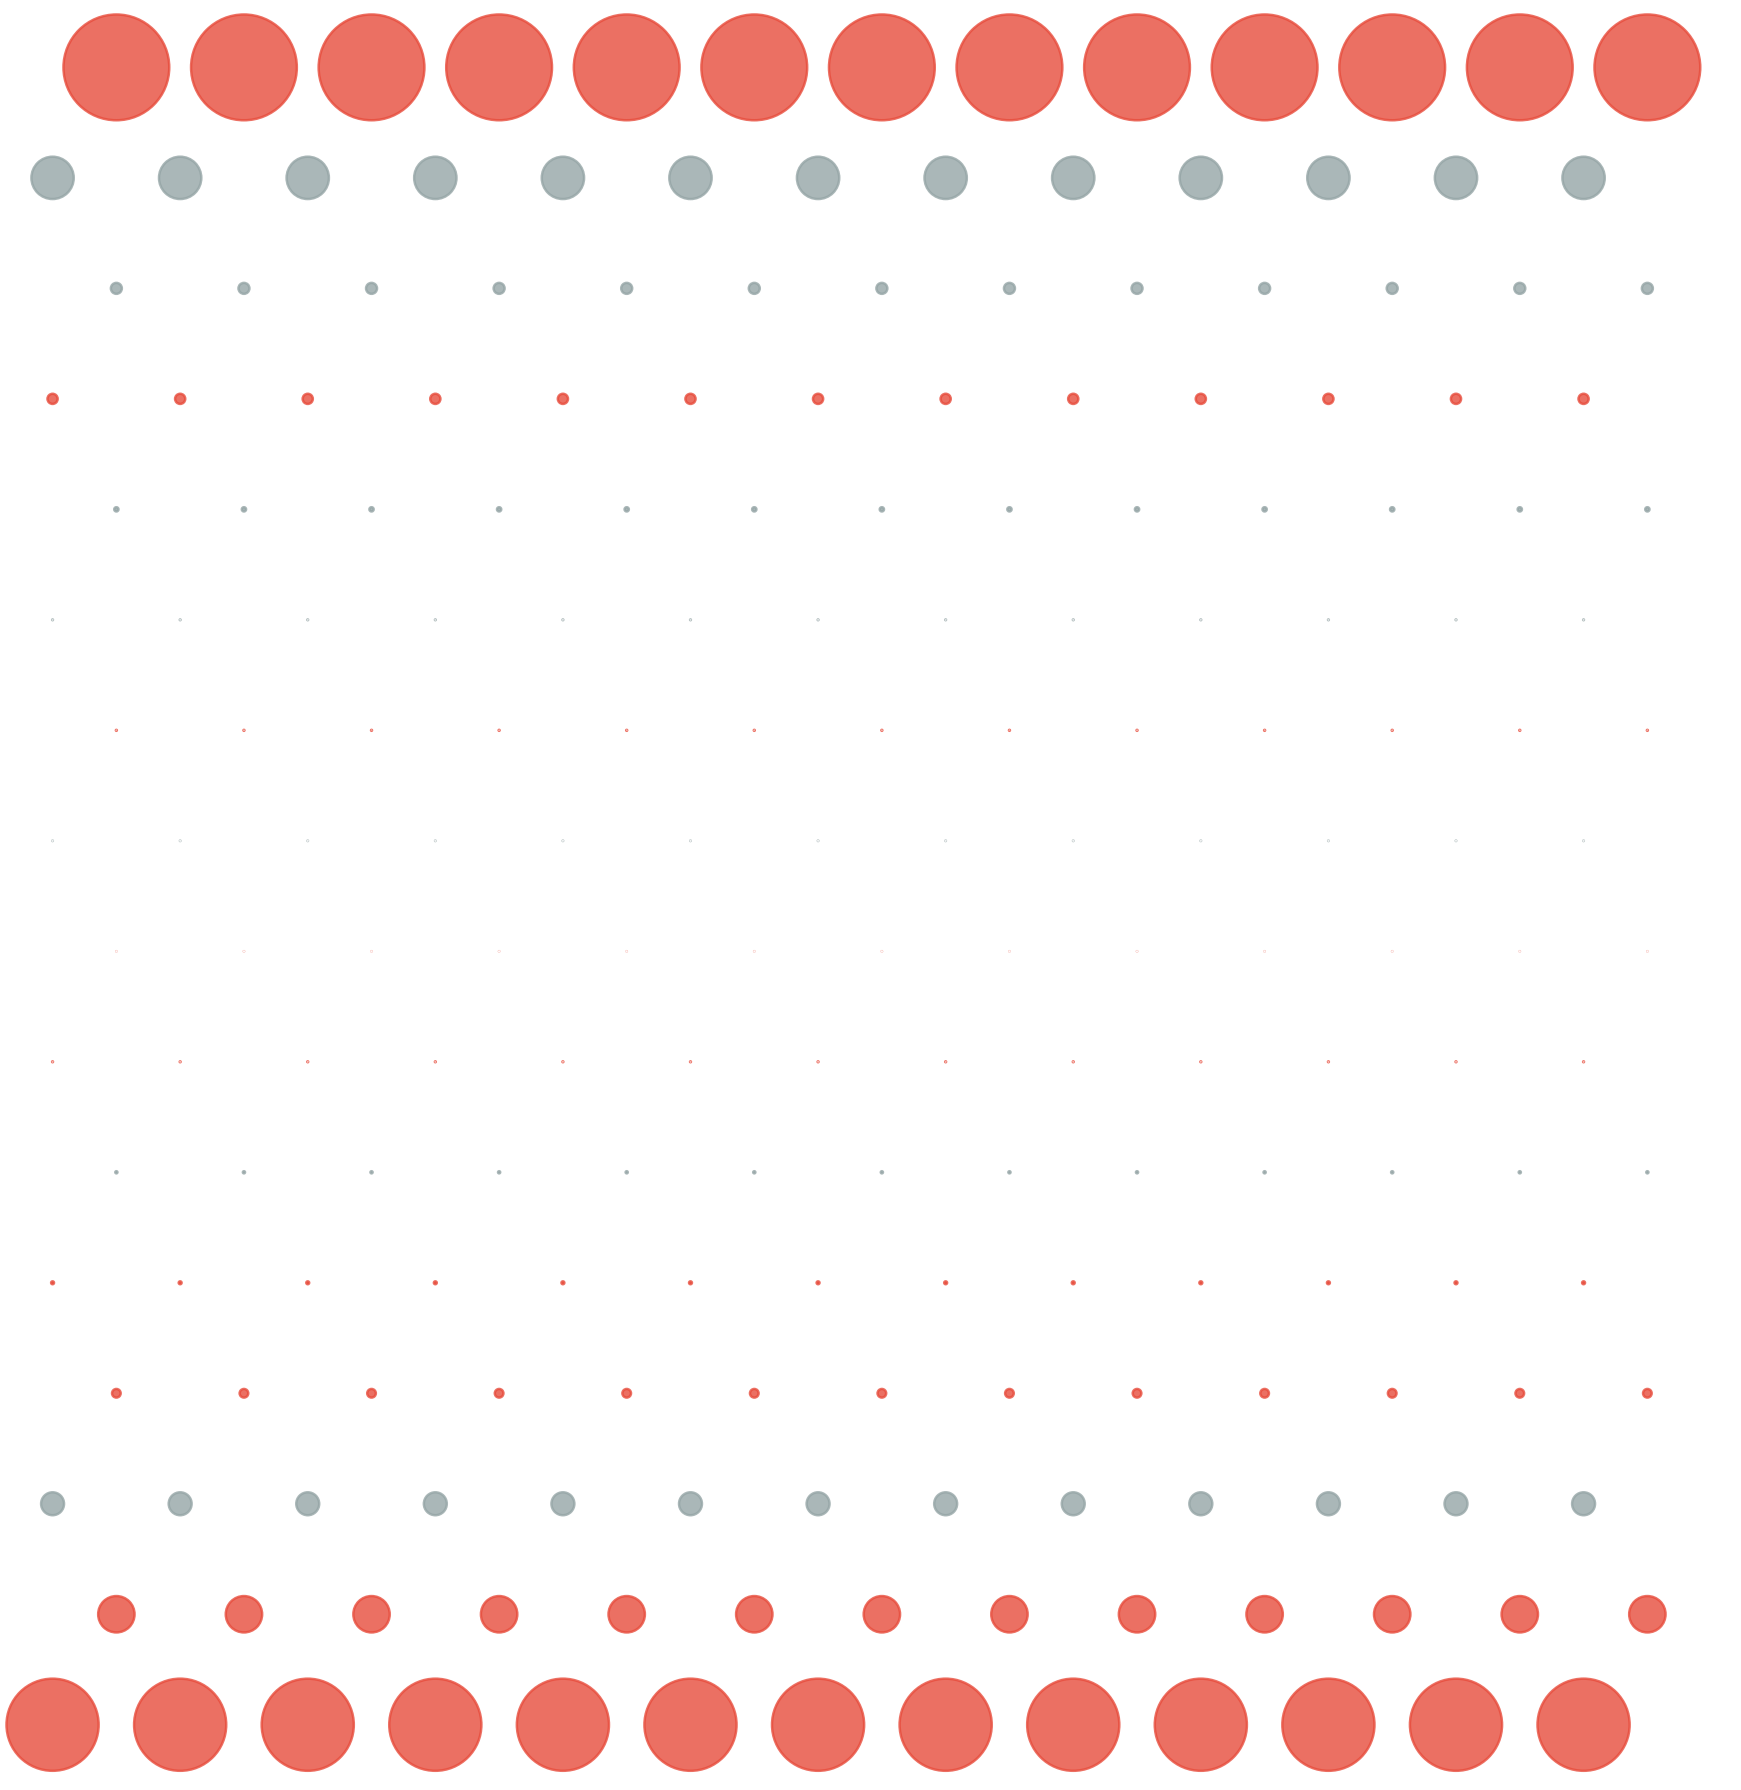
\includegraphics[scale=0.55]{Applications/lattice_Nx=512_Ny=16_U=20_beta=100.png}
\hspace{1cm}
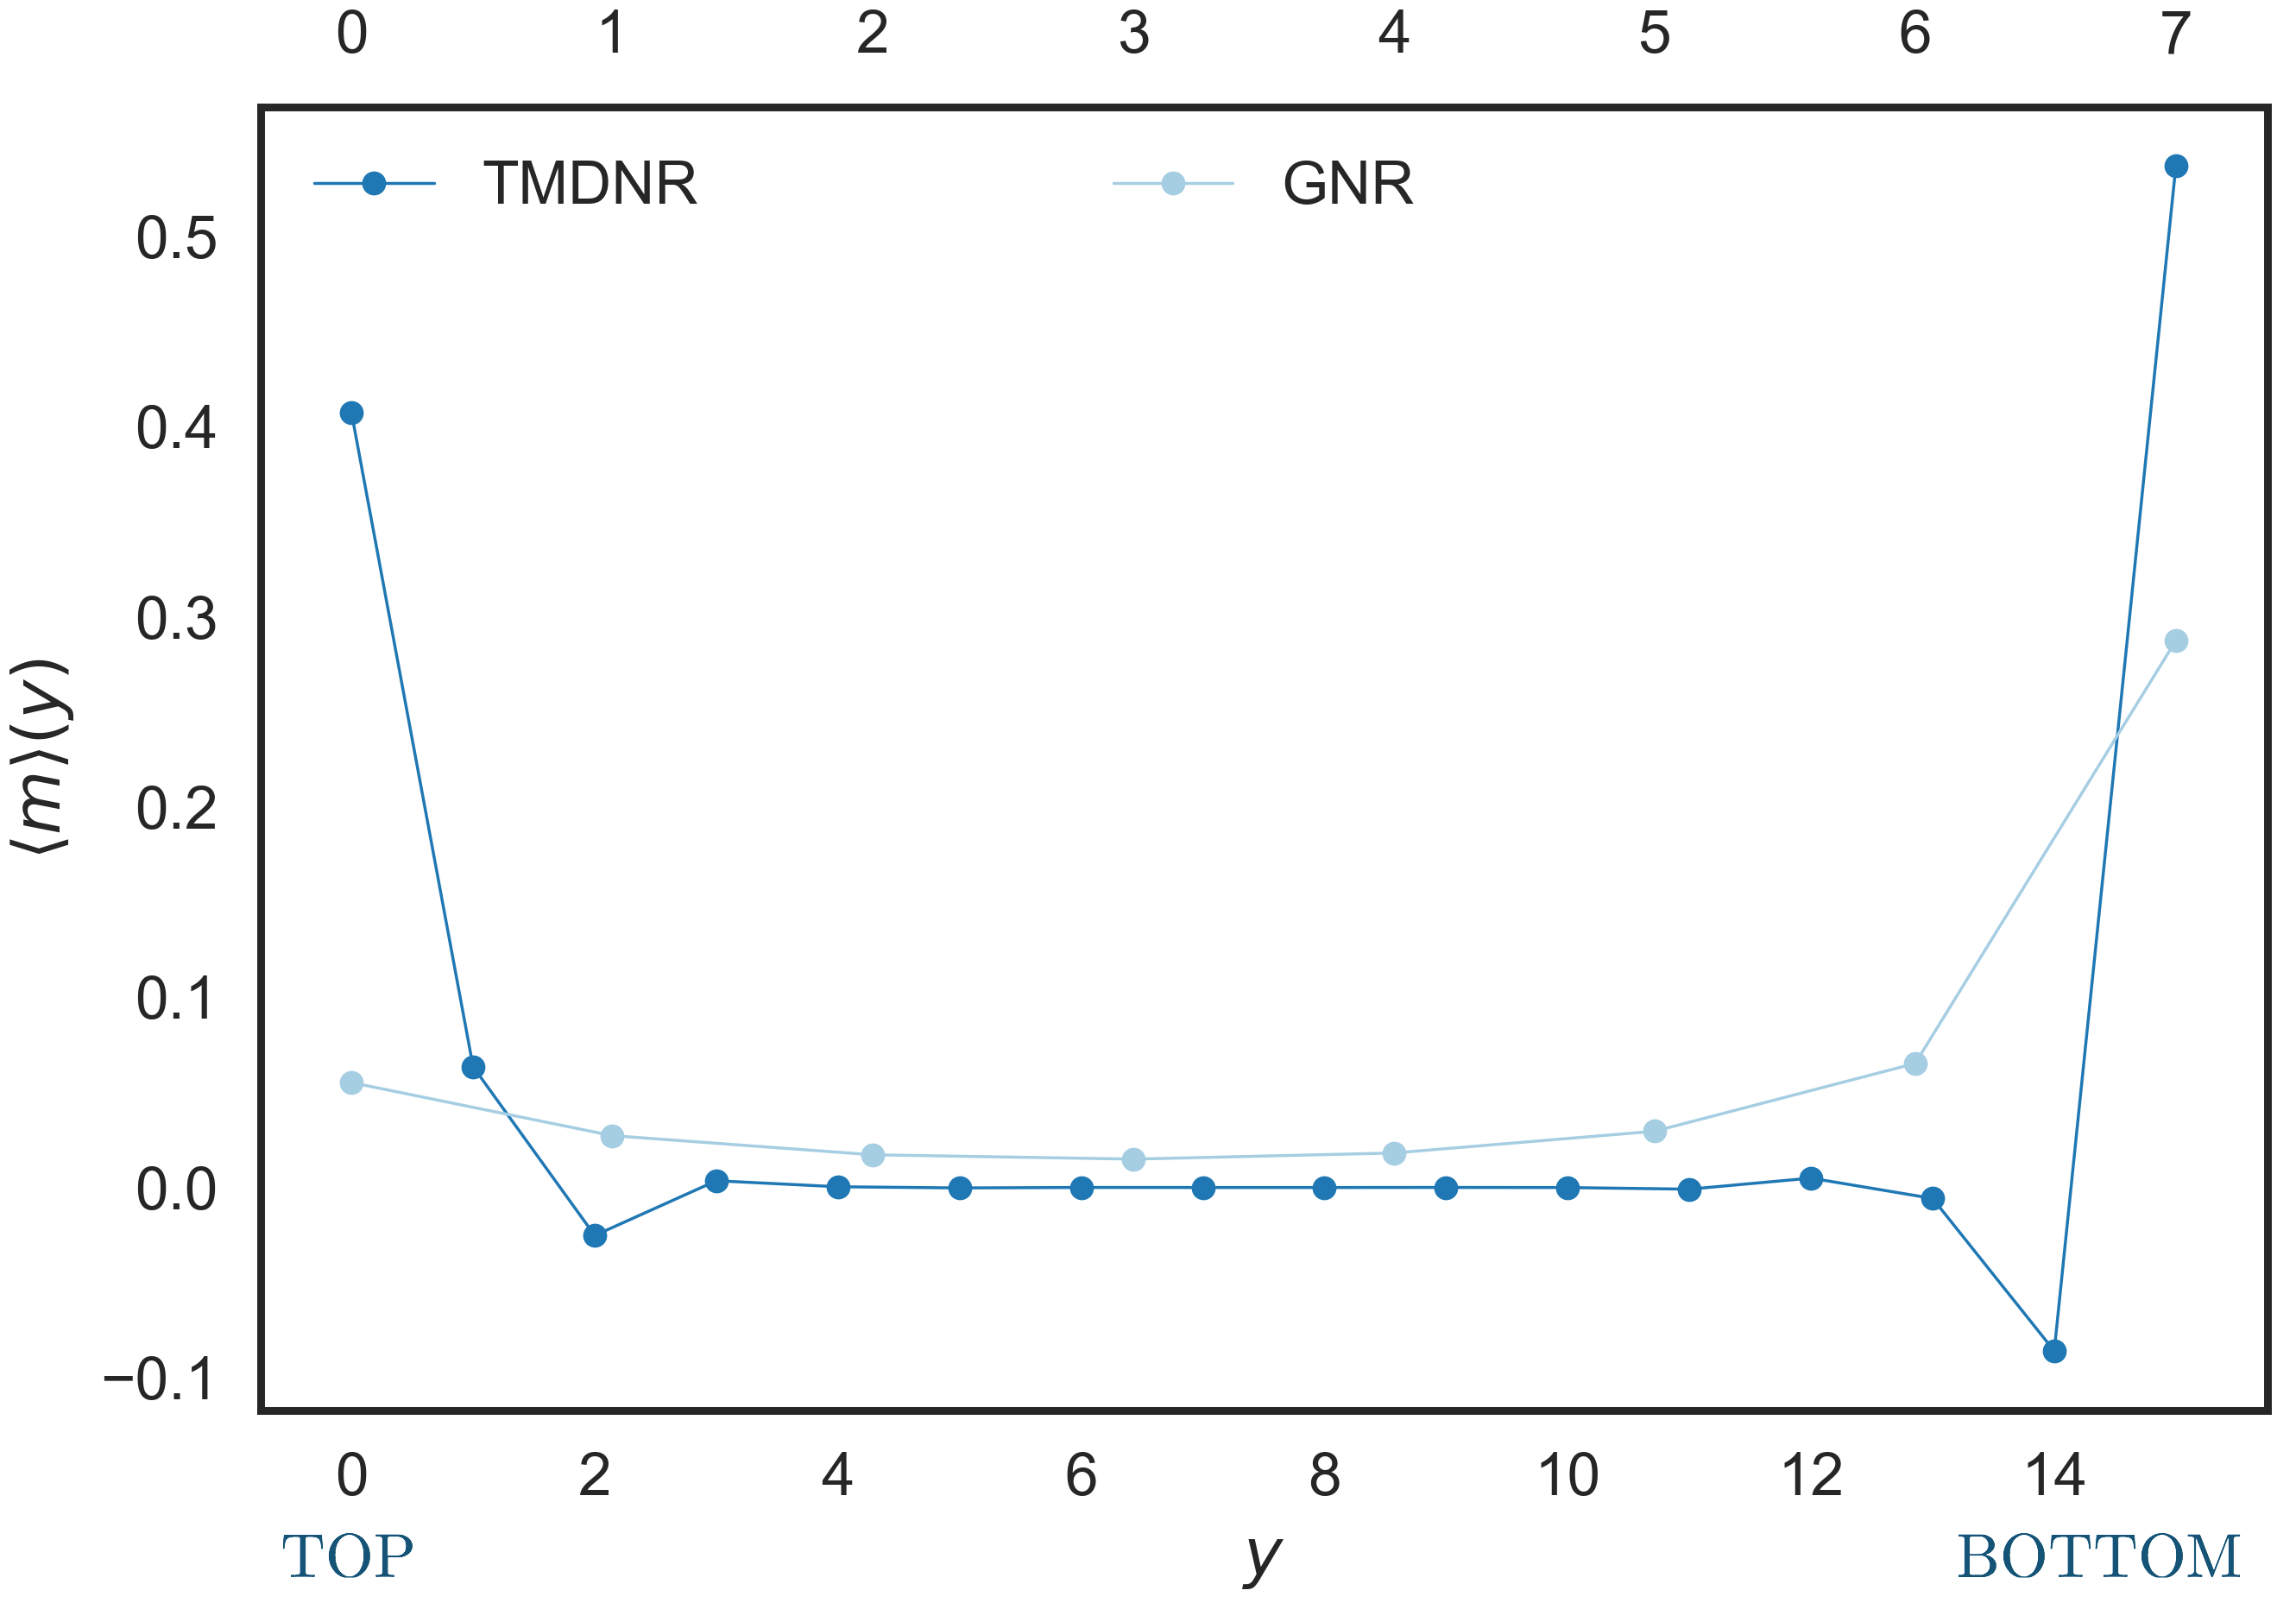
\includegraphics[scale=0.462]{Applications/magProf.png}
	\caption[Comparison between the MF solutions of the Hubbard model for a graphene nanoribbon (GNR) and a \acs{TMDNR}. Spin density profile along the ribbon's transverse direction.]{Left: Comparison between the MF solutions of the Hubbard model at half filling for a graphene nanoribbon (GNR) at $U=1.2$ with $\beta t = 20$ (left) and a \acs{TMDNR}.
	Right: Comparison between the spin density profile along the ribbon's transverse direction $\left\langle m \right\rangle (y)$ (the obtained solution is constant along $x$) for the GNR and the \acs{TMDNR}).}
	\label{fig:nanoGraphVsTMD}
\end{figure}
\begin{figure}[H]
\centering
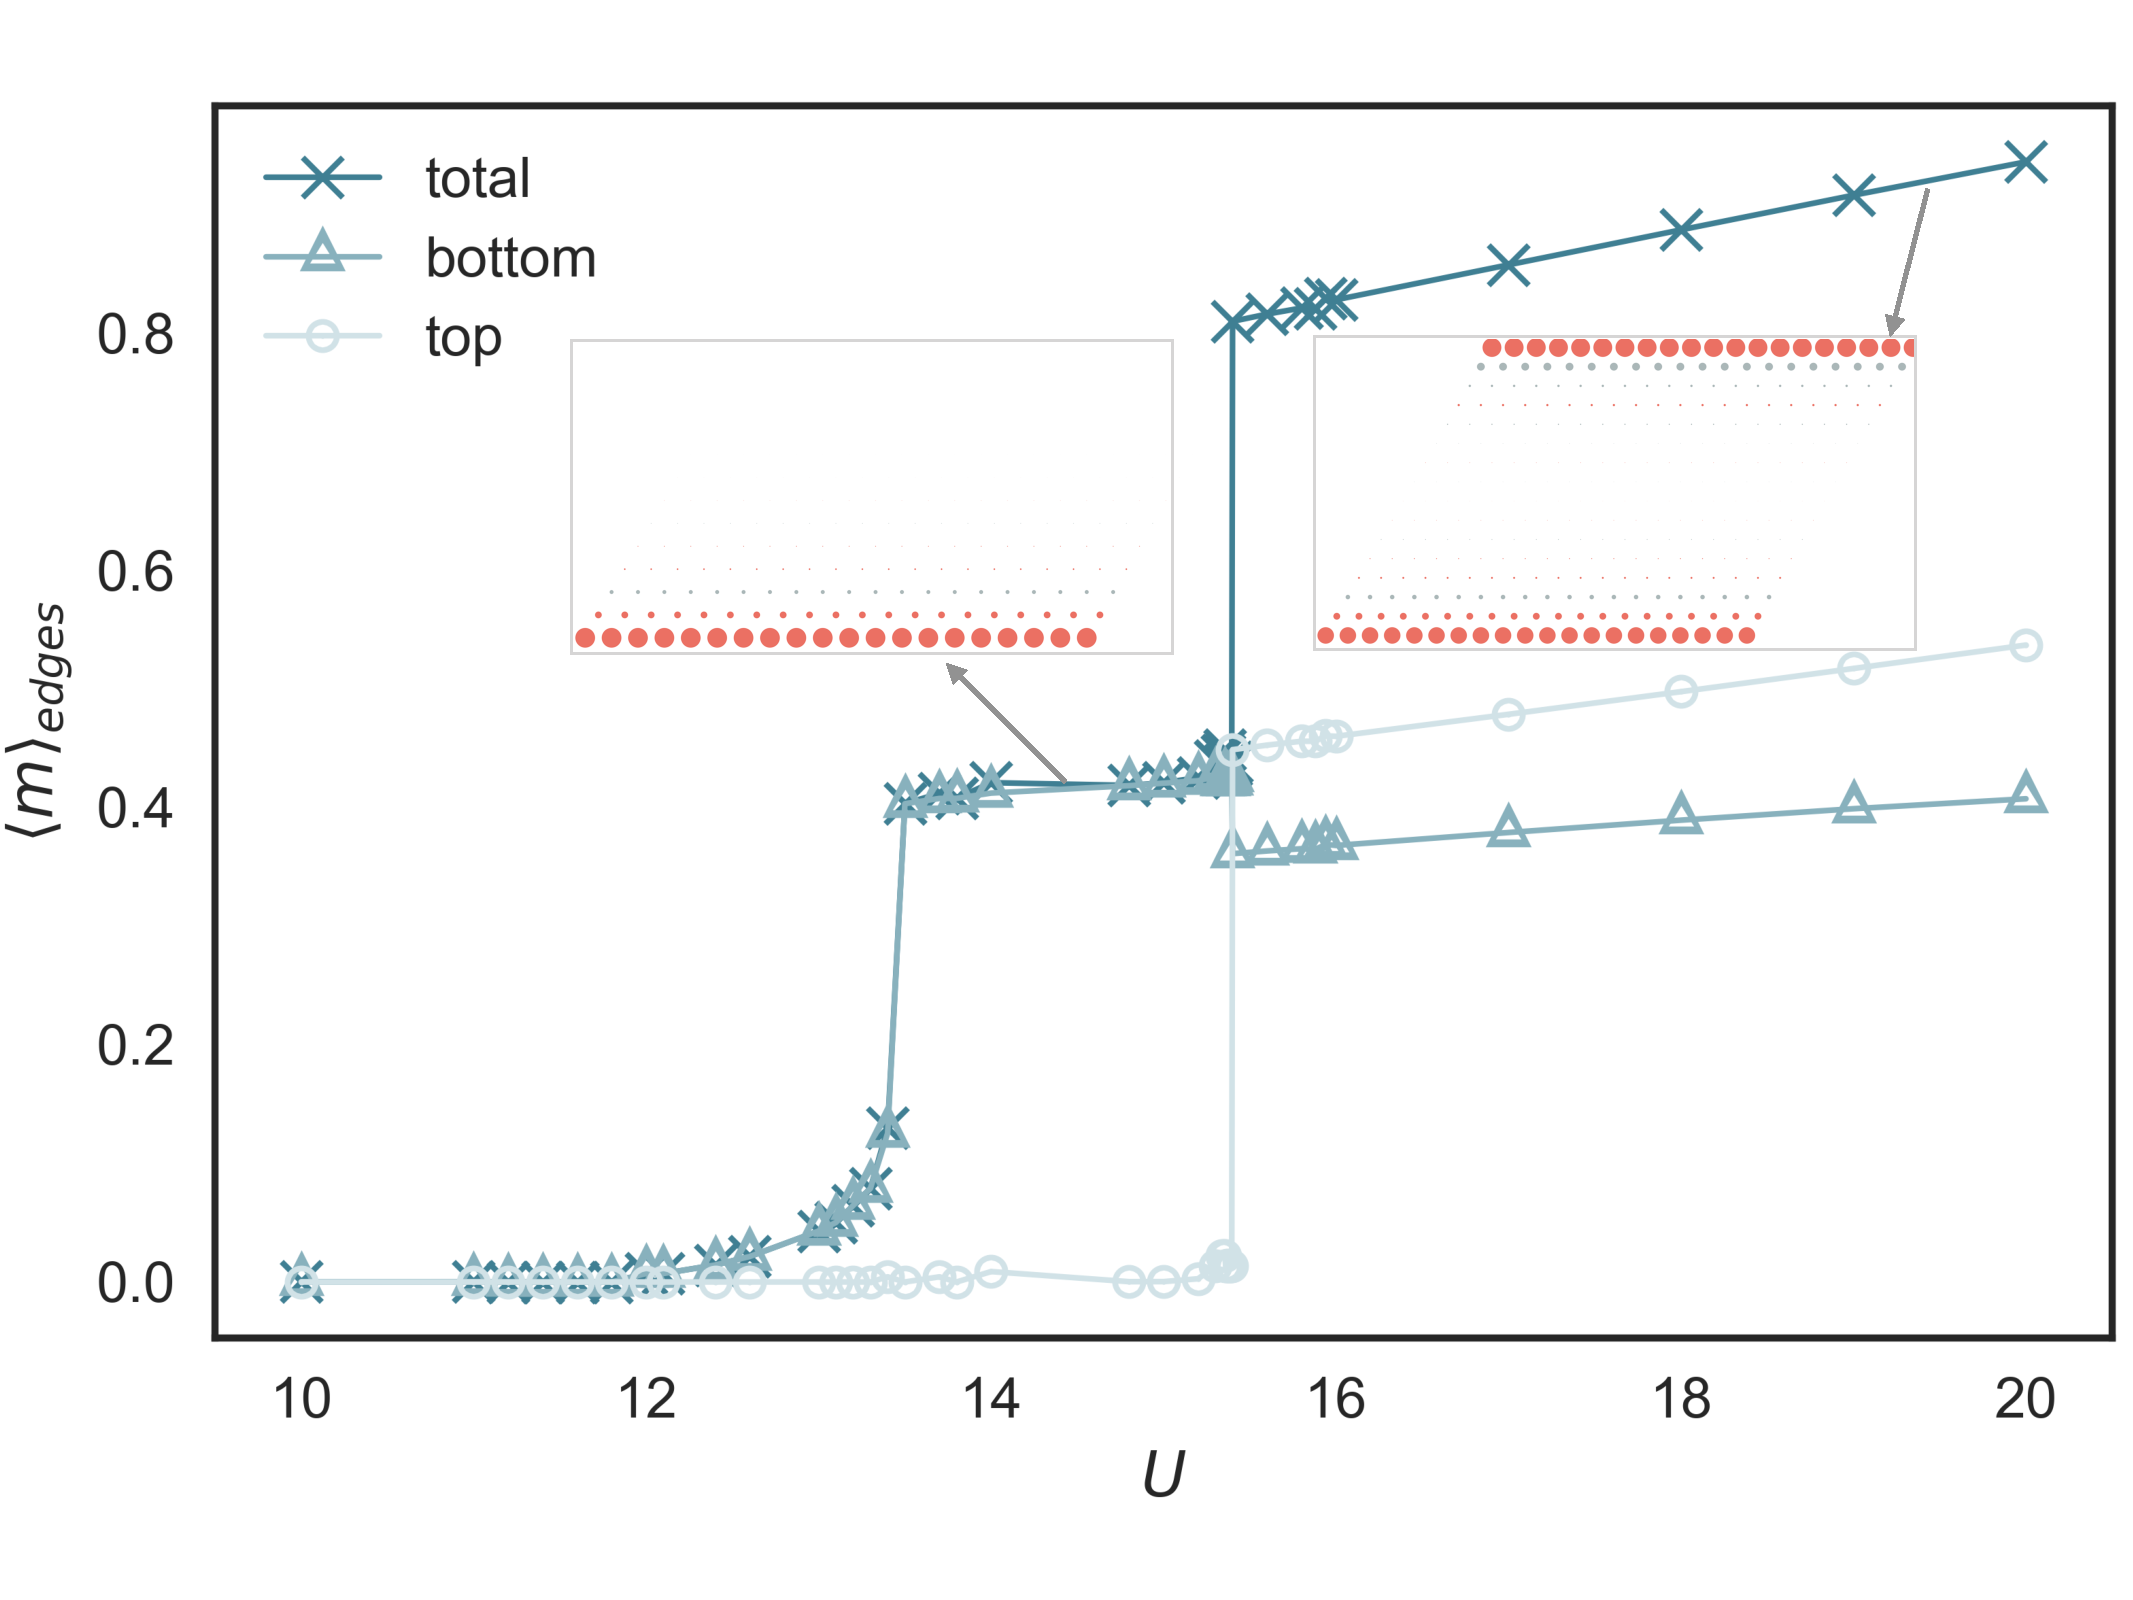
\includegraphics[trim={0cm 1.5cm 0cm 1.5cm},clip, scale =0.23]{Applications/tmd-mf/edge-mag.pdf}
	\caption[]{}
	\label{fig:zeroTphaseDiagram}
\end{figure}
\begin{figure}[H]
\centering
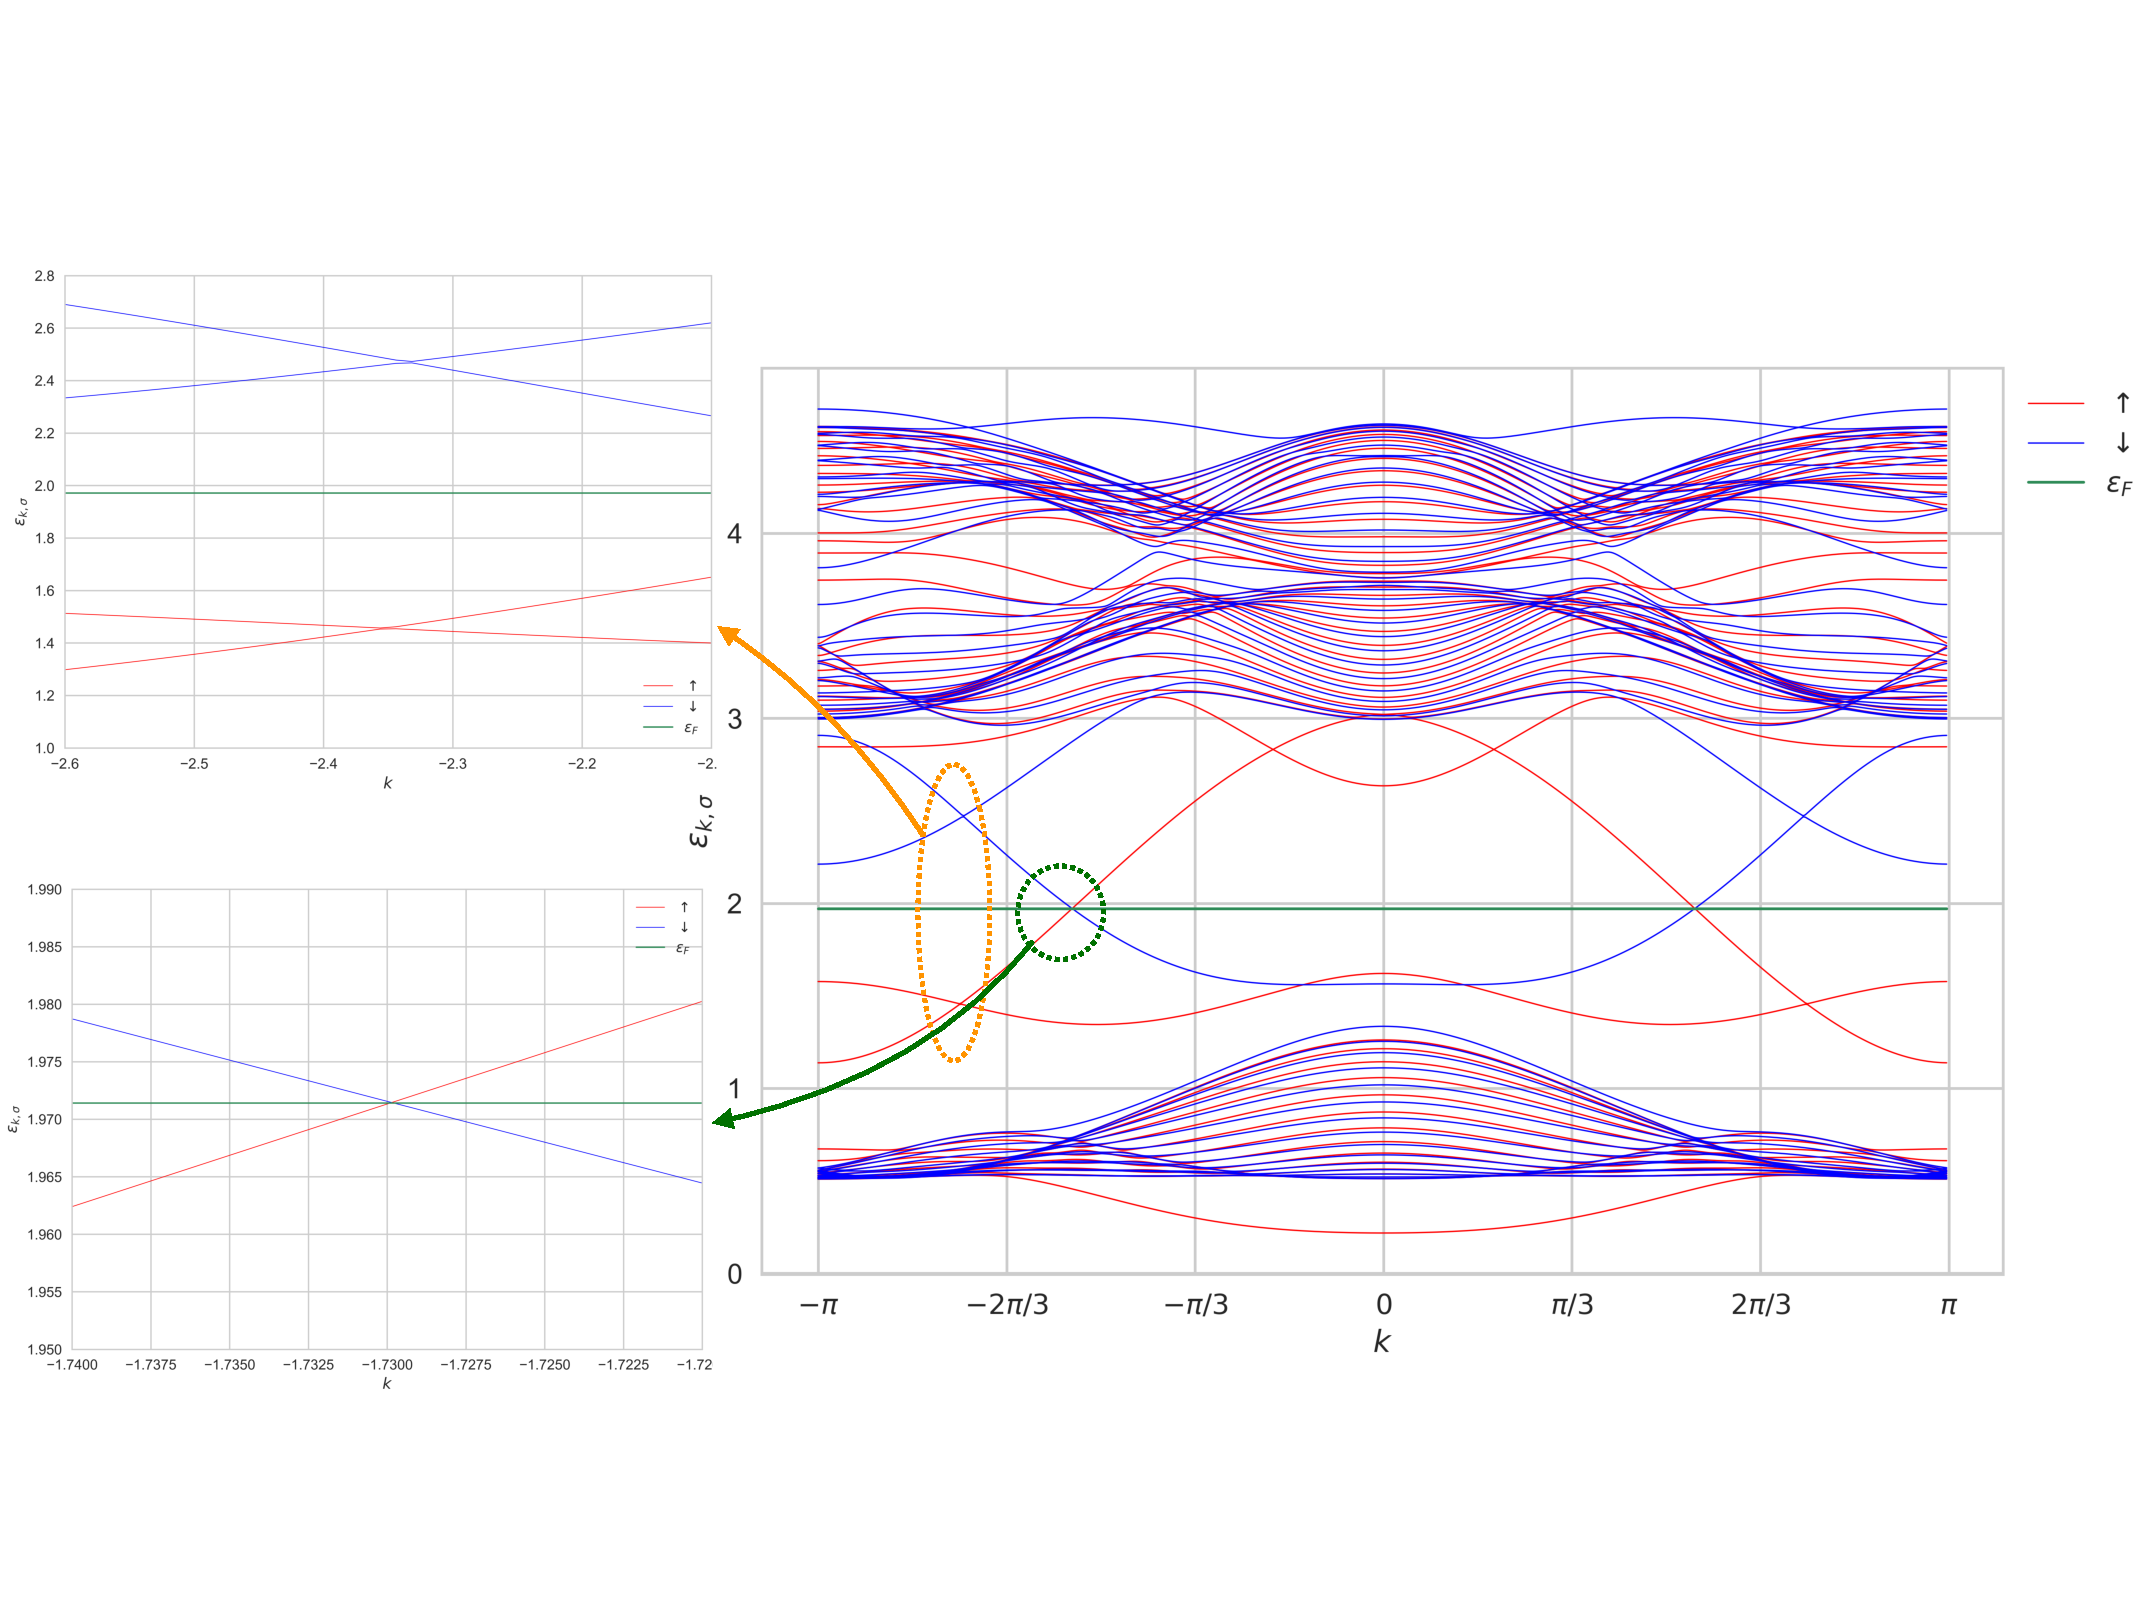
\includegraphics[trim={0cm 1.5cm 0cm 1.5cm},clip, scale =0.3]{Applications/tmd-mf/bandsZoomed.pdf}
	\caption[]{}
	\label{fig:bandsZoomed}
\end{figure}
\begin{figure}[H]
\centering
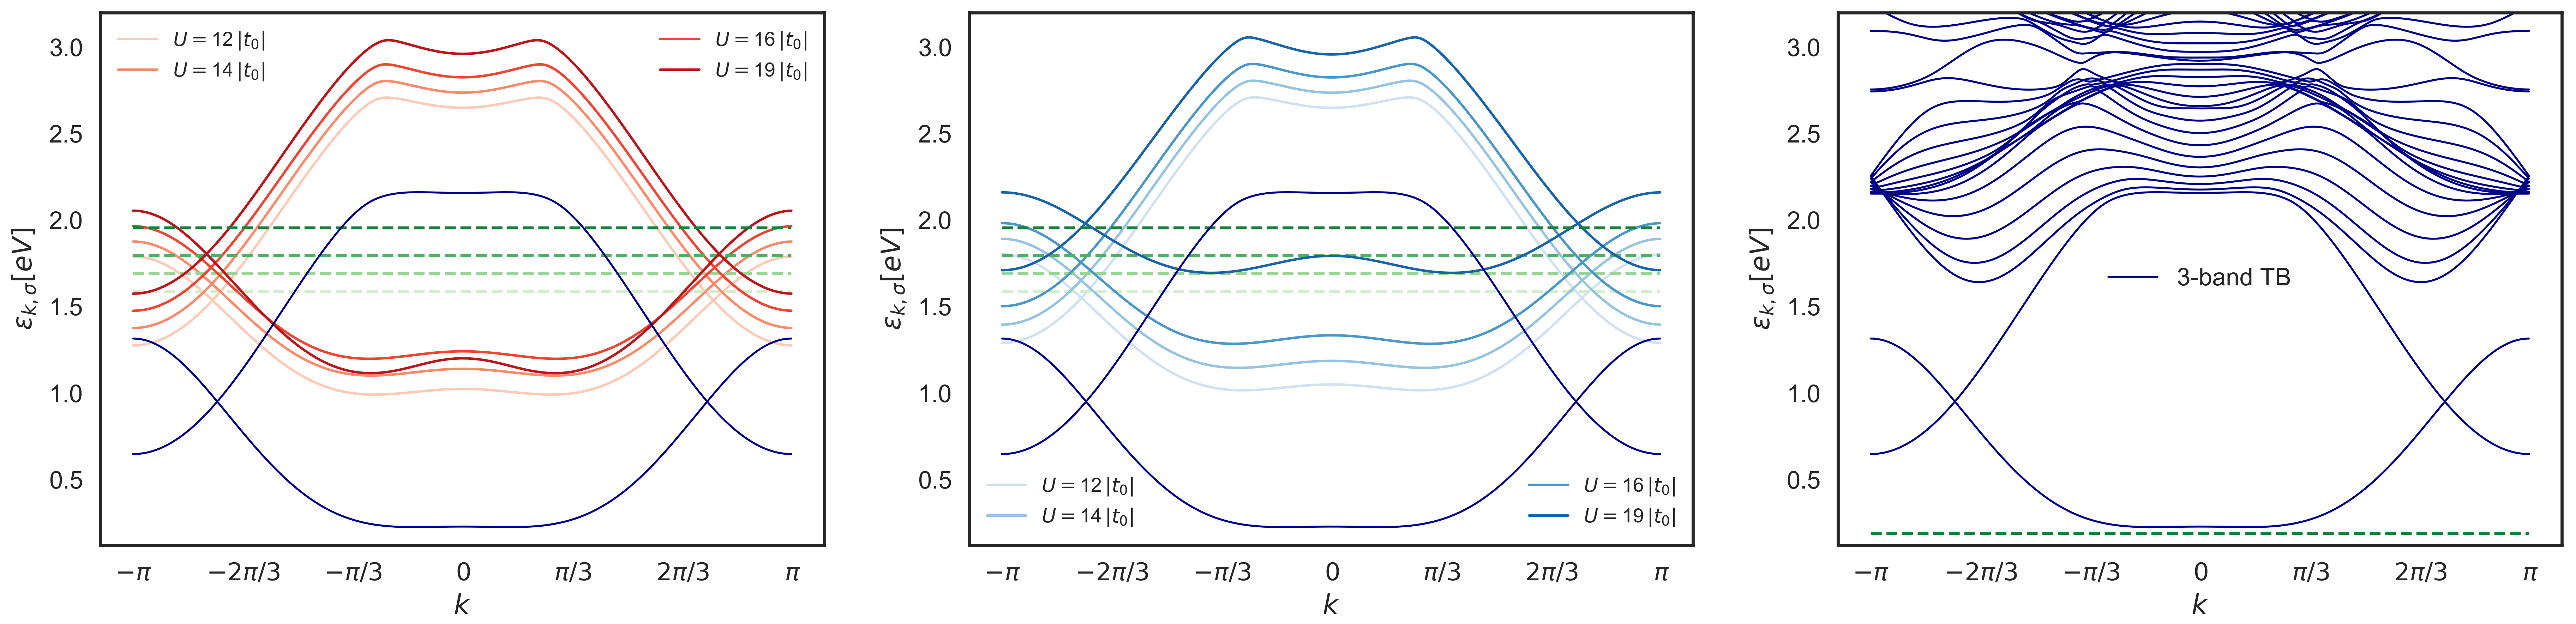
\includegraphics[scale=0.4]{Applications/tmd-mf/superposedBands05} \\
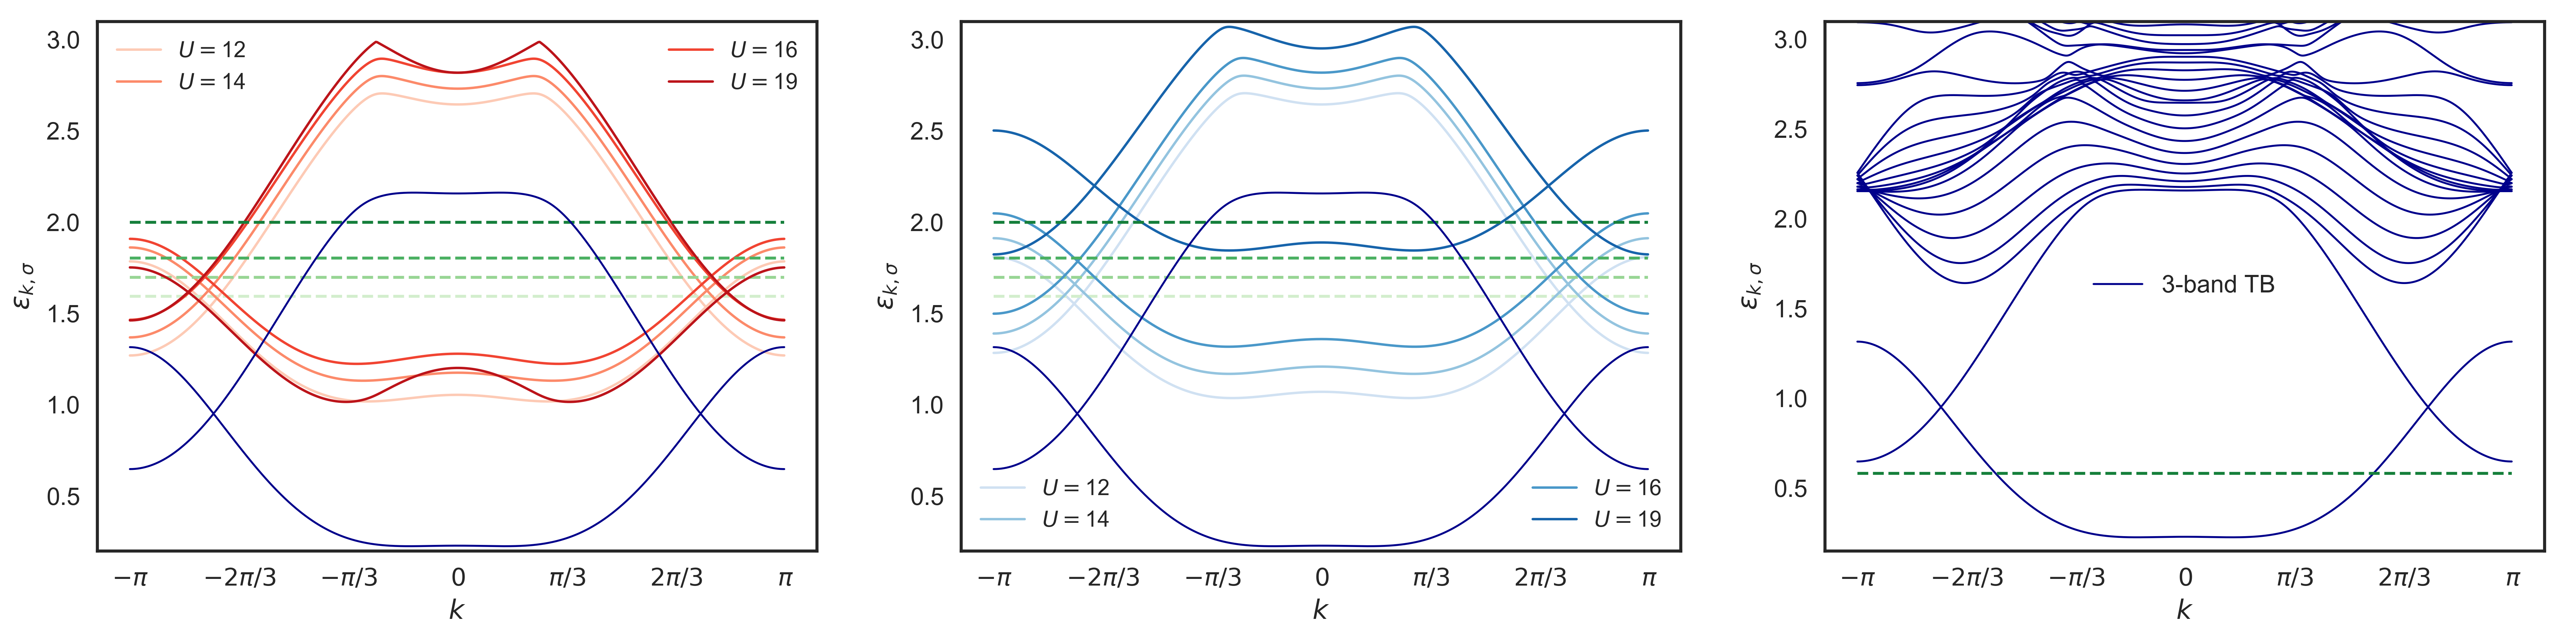
\includegraphics[scale=0.4]{Applications/tmd-mf/superposedBands075} \\
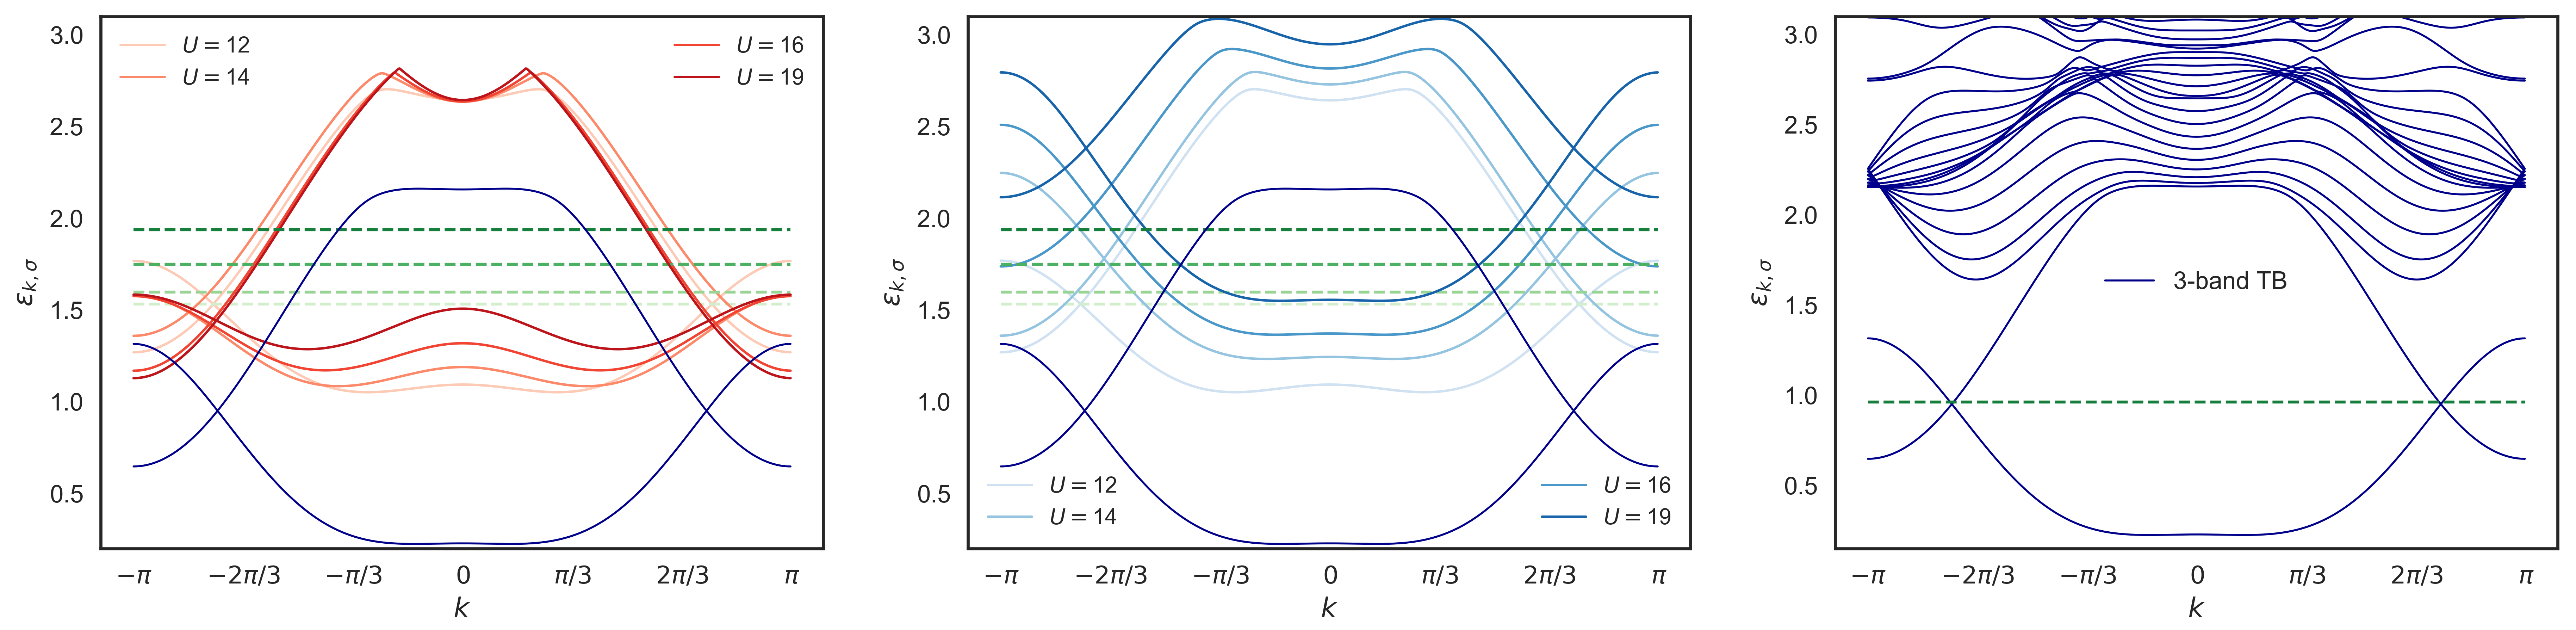
\includegraphics[scale=0.4]{Applications/tmd-mf/superposedBands4} \\
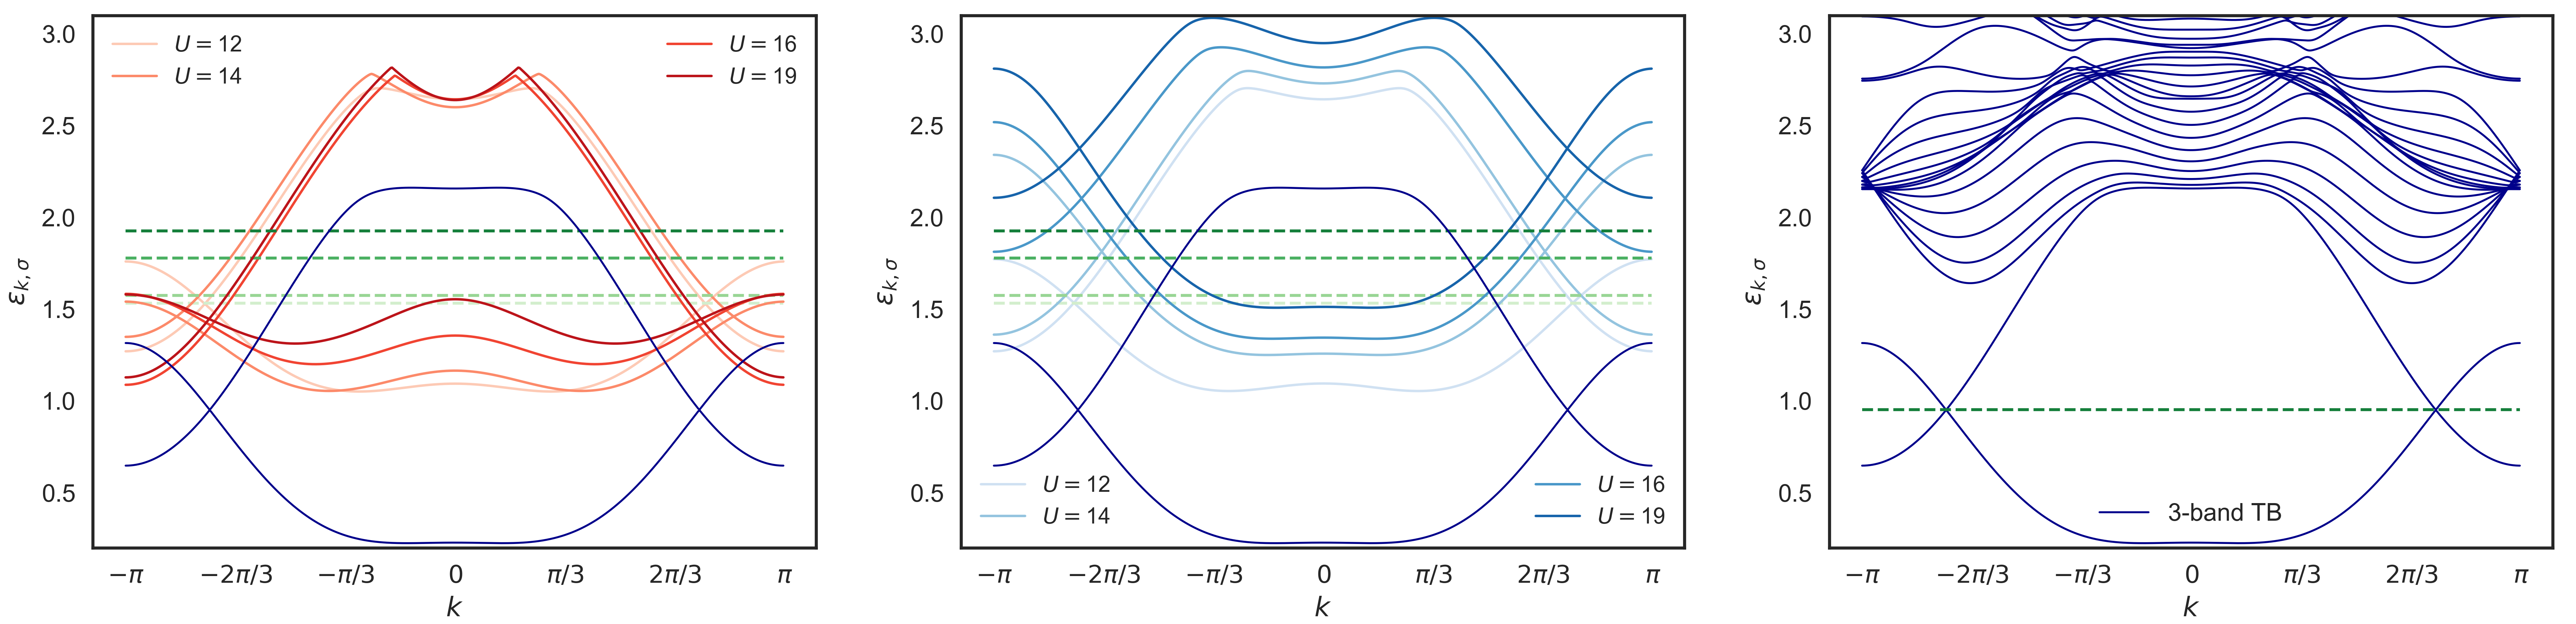
\includegraphics[scale=0.4]{Applications/tmd-mf/superposedBands100} \\
	\caption[]{}
	\label{fig:band-structures}
\end{figure}
\begin{figure}[H]
\hspace{1cm}
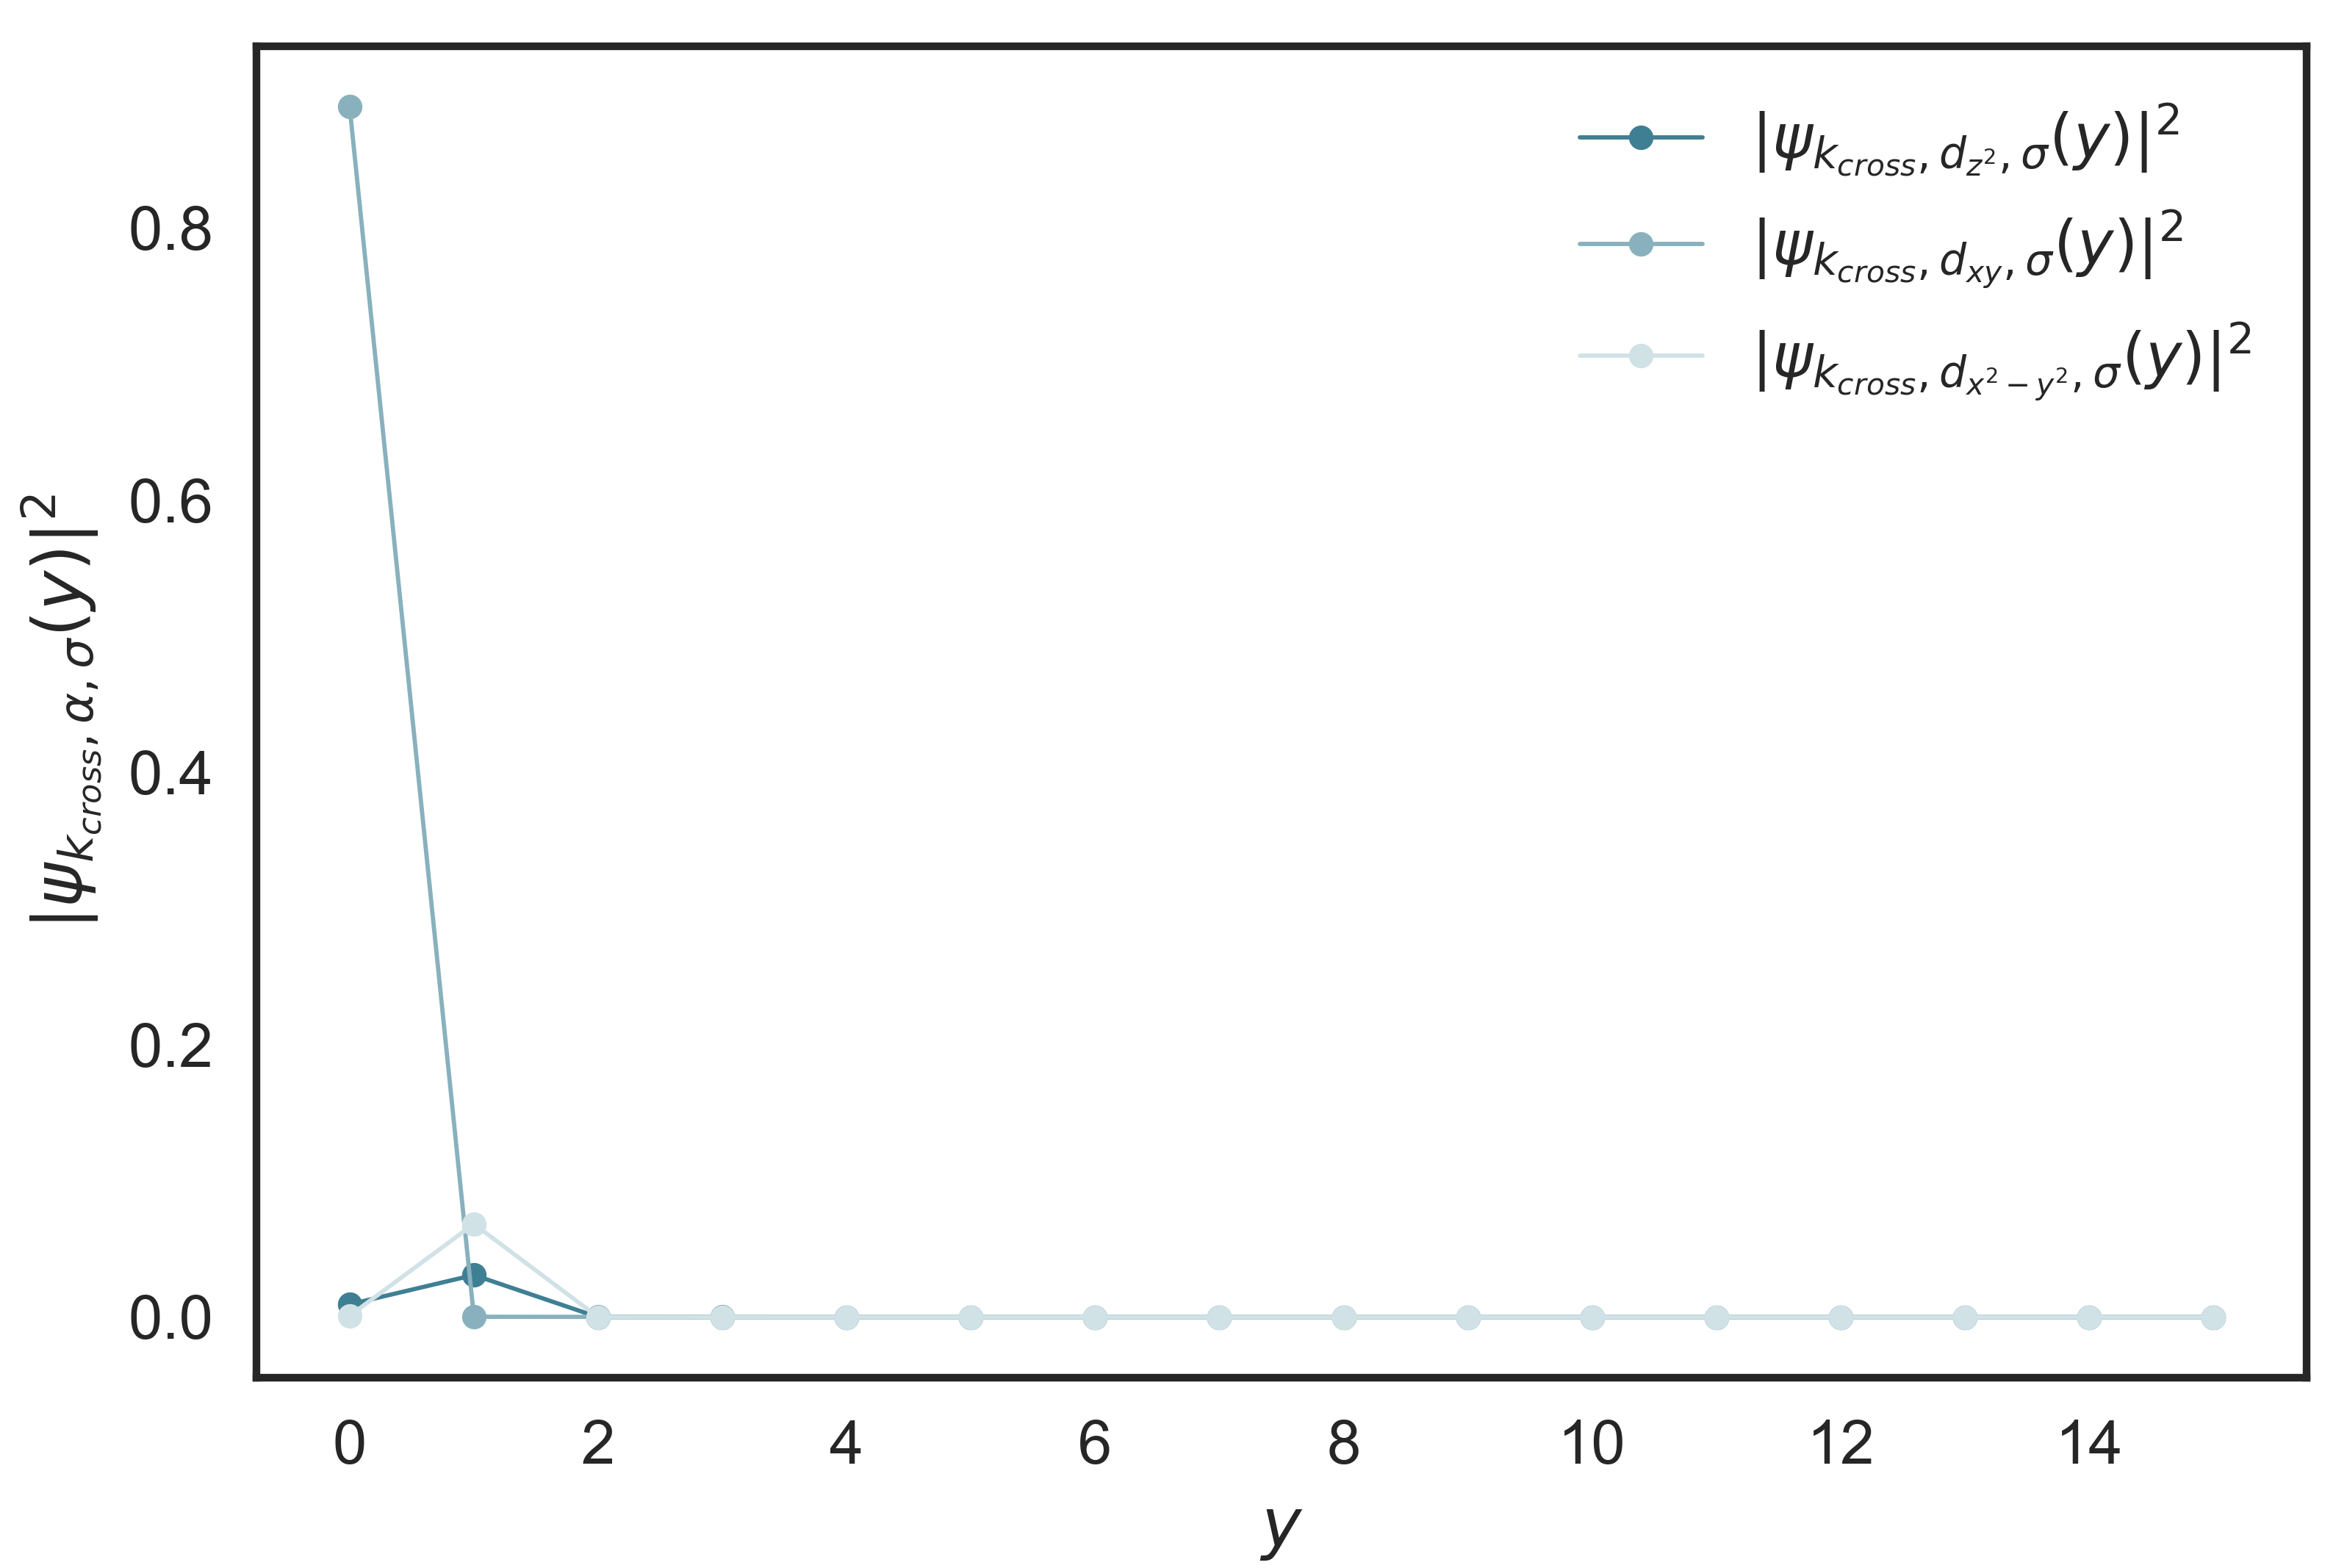
\includegraphics[scale=0.5]{Applications/tmd-mf/wfAroundK1}
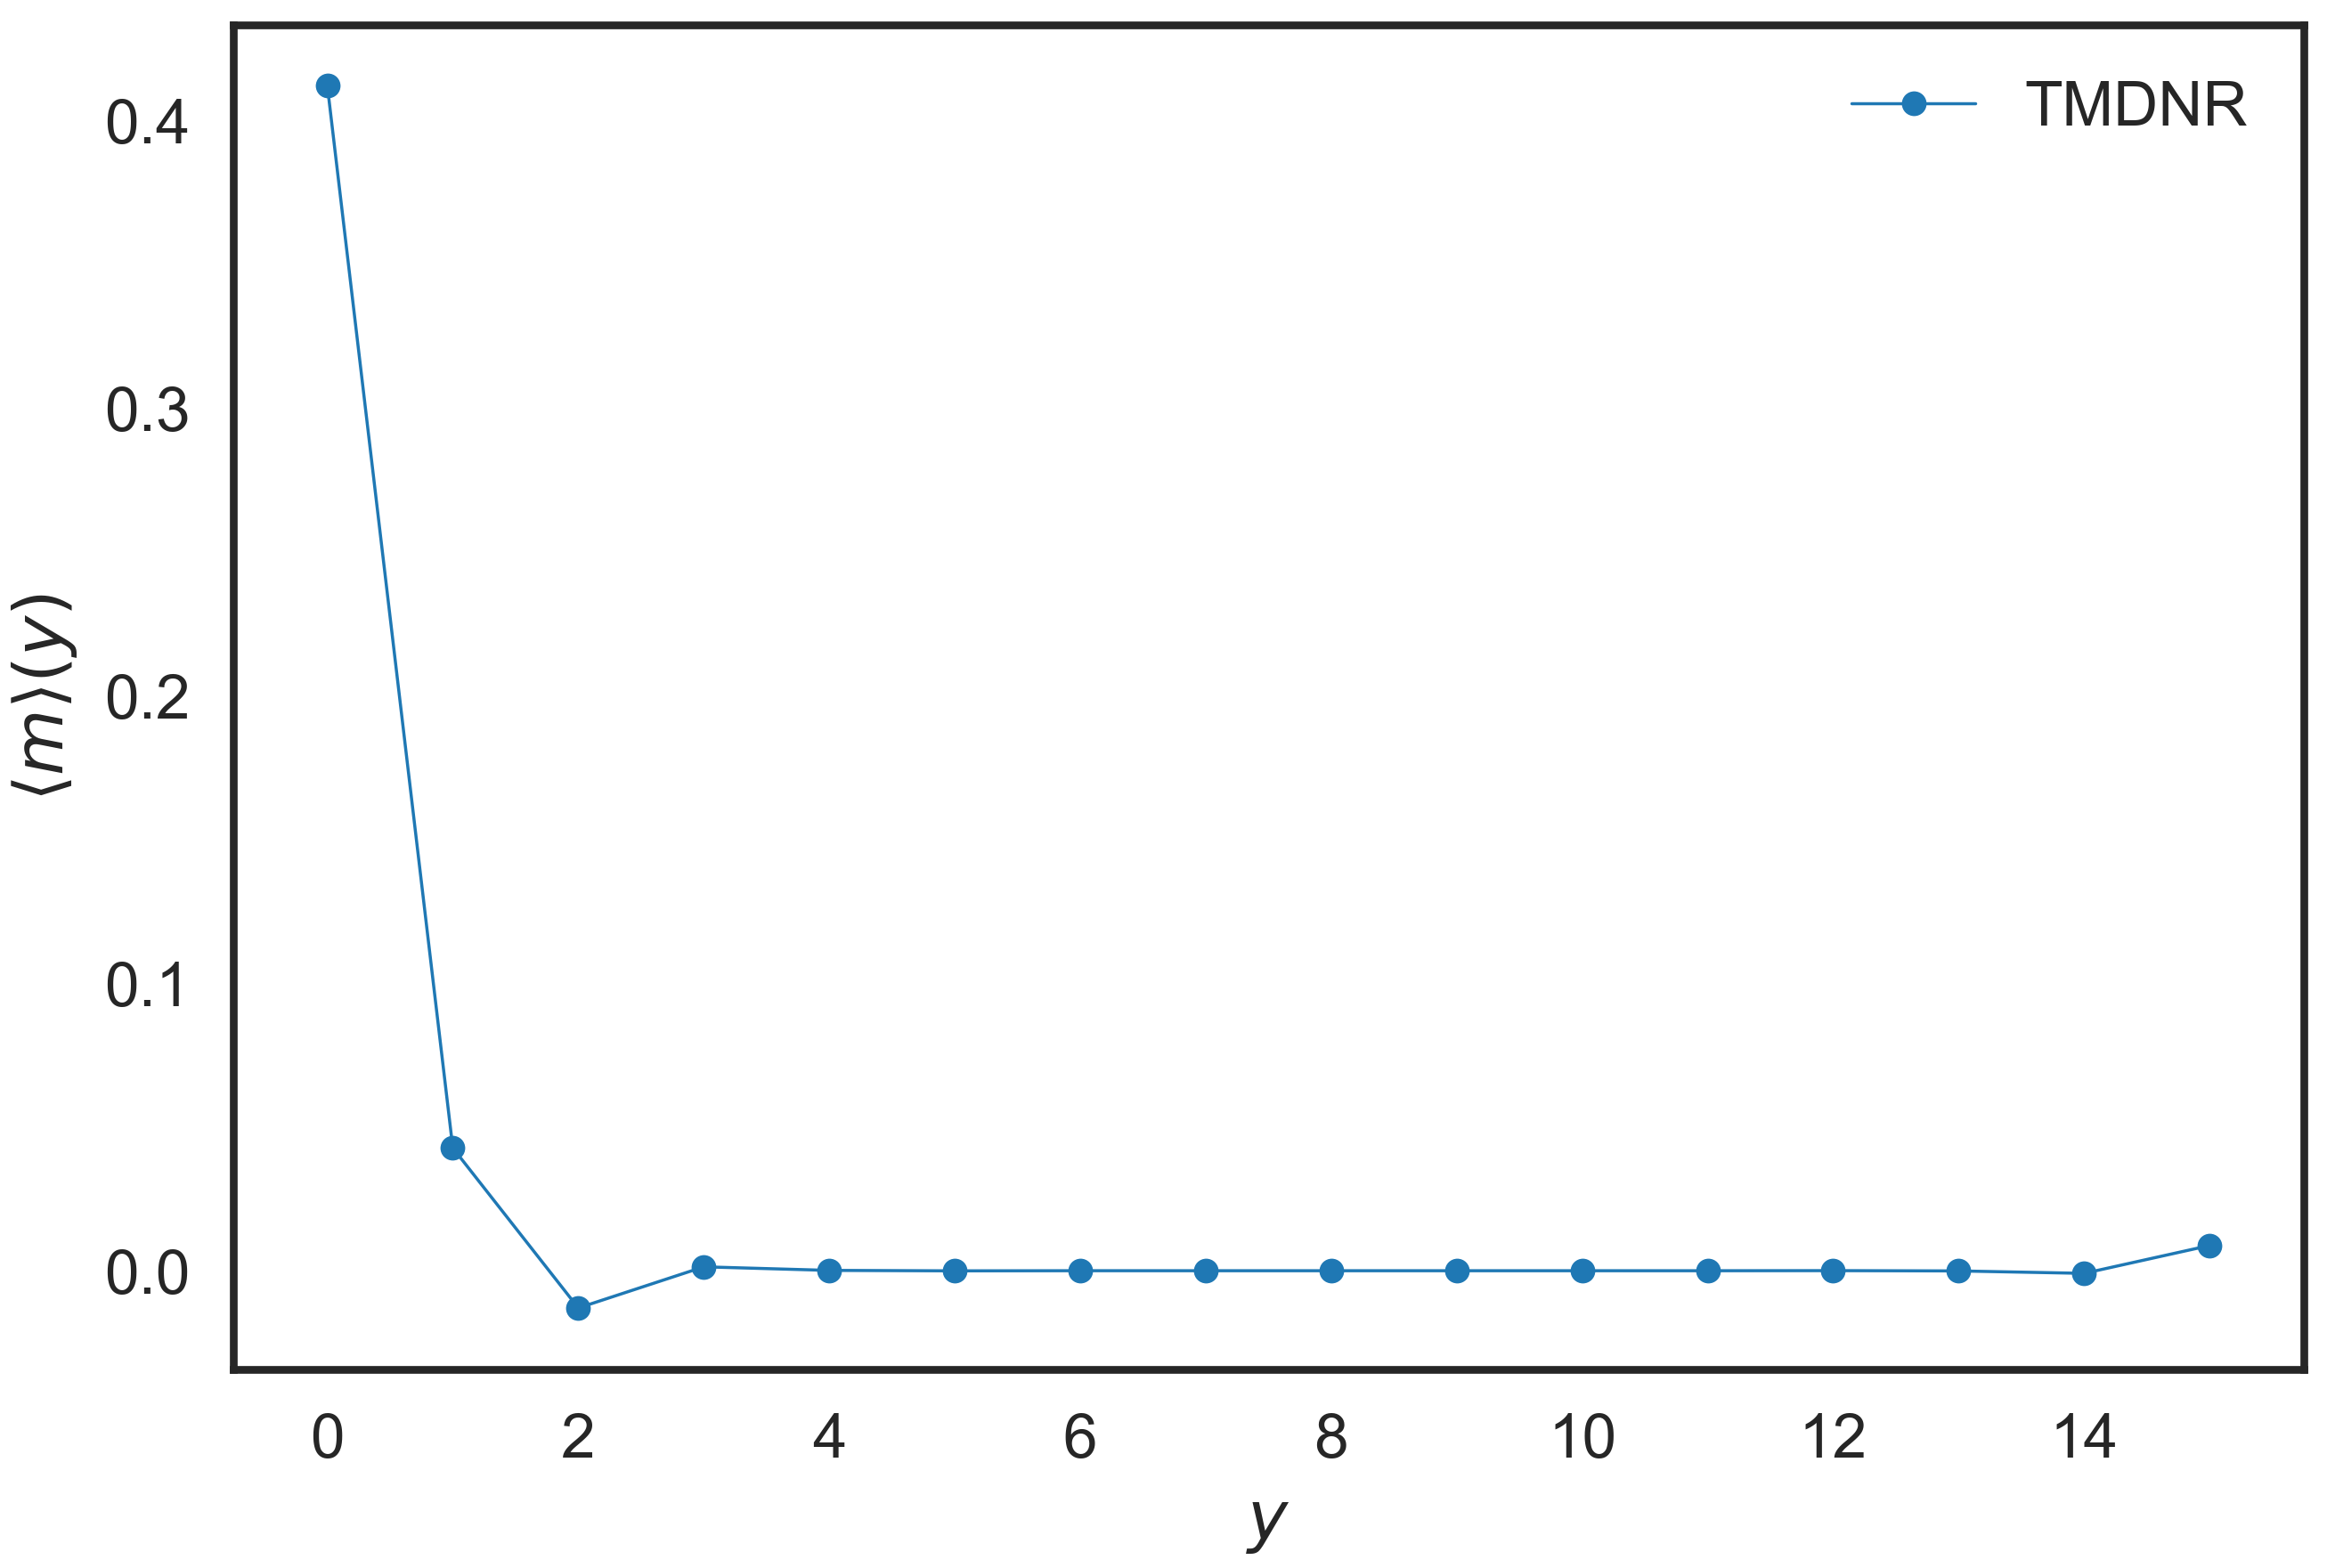
\includegraphics[scale=0.5]{Applications/tmd-mf/magProfU14}
	\caption[]{}
	\label{fig:wfs}
\end{figure}
\begin{figure}[H]
\hspace{1.2cm}
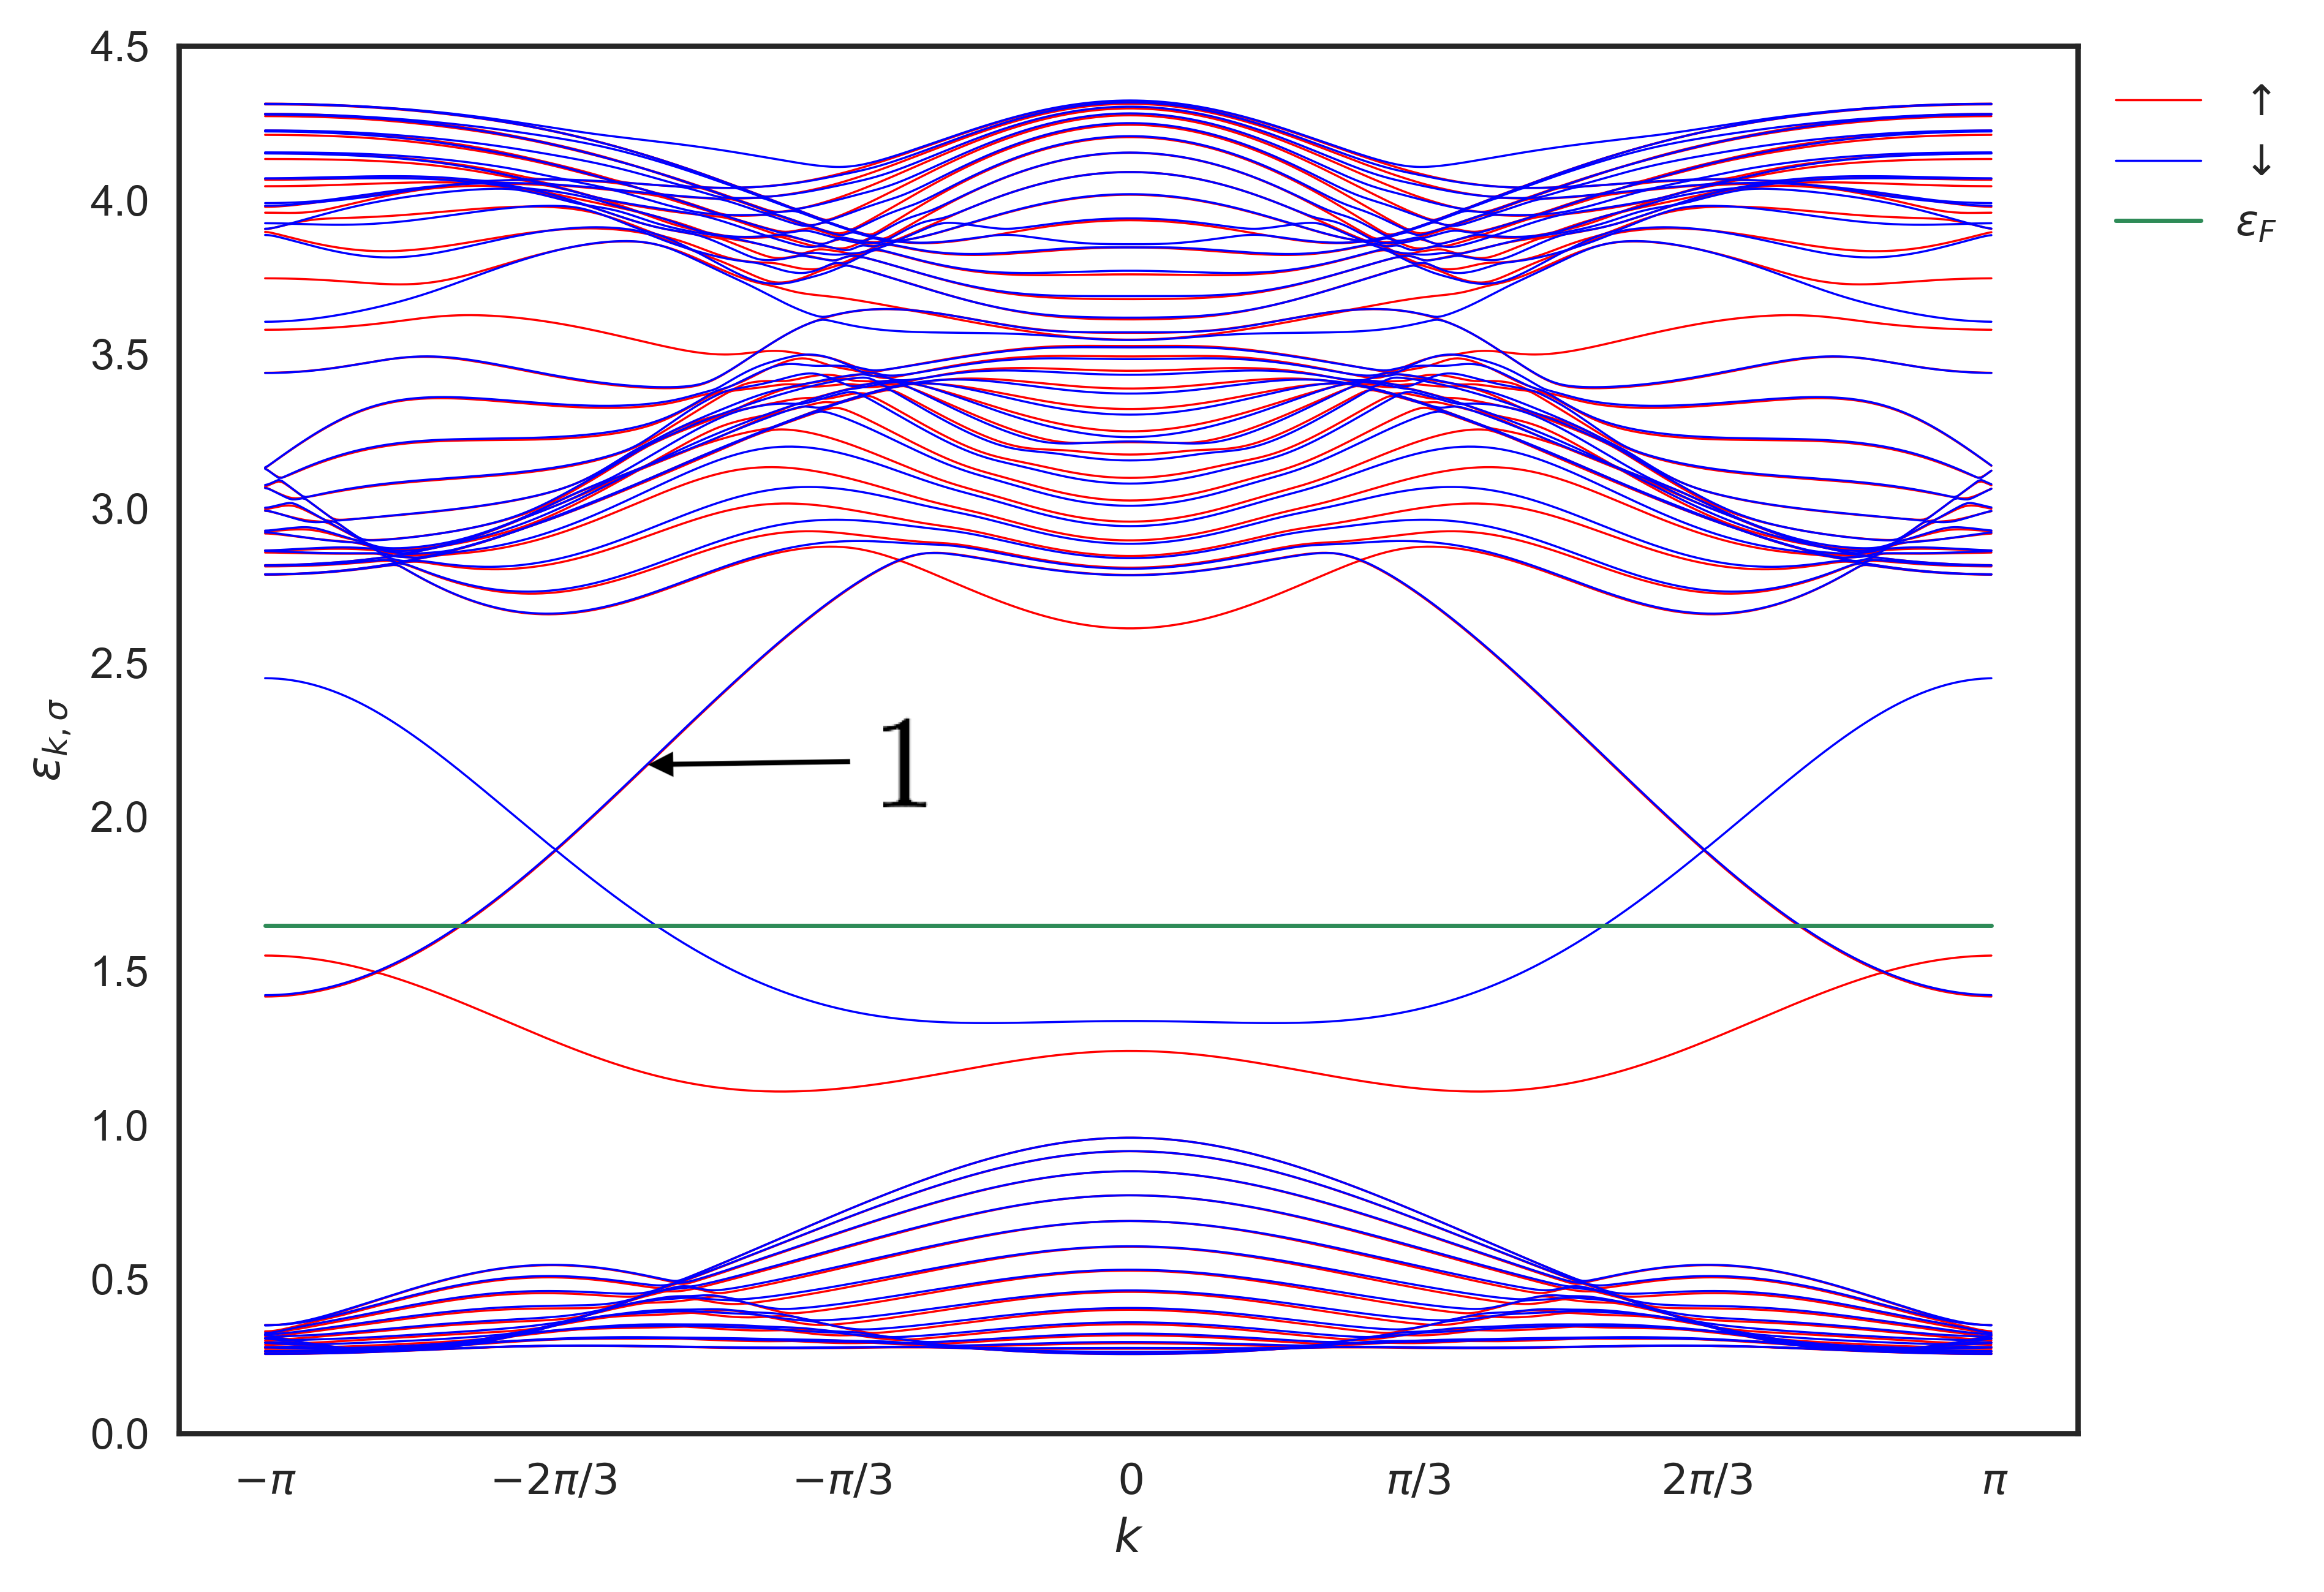
\includegraphics[scale=0.35]{Applications/tmd-mf/bands152.png}
\hspace{4mm}
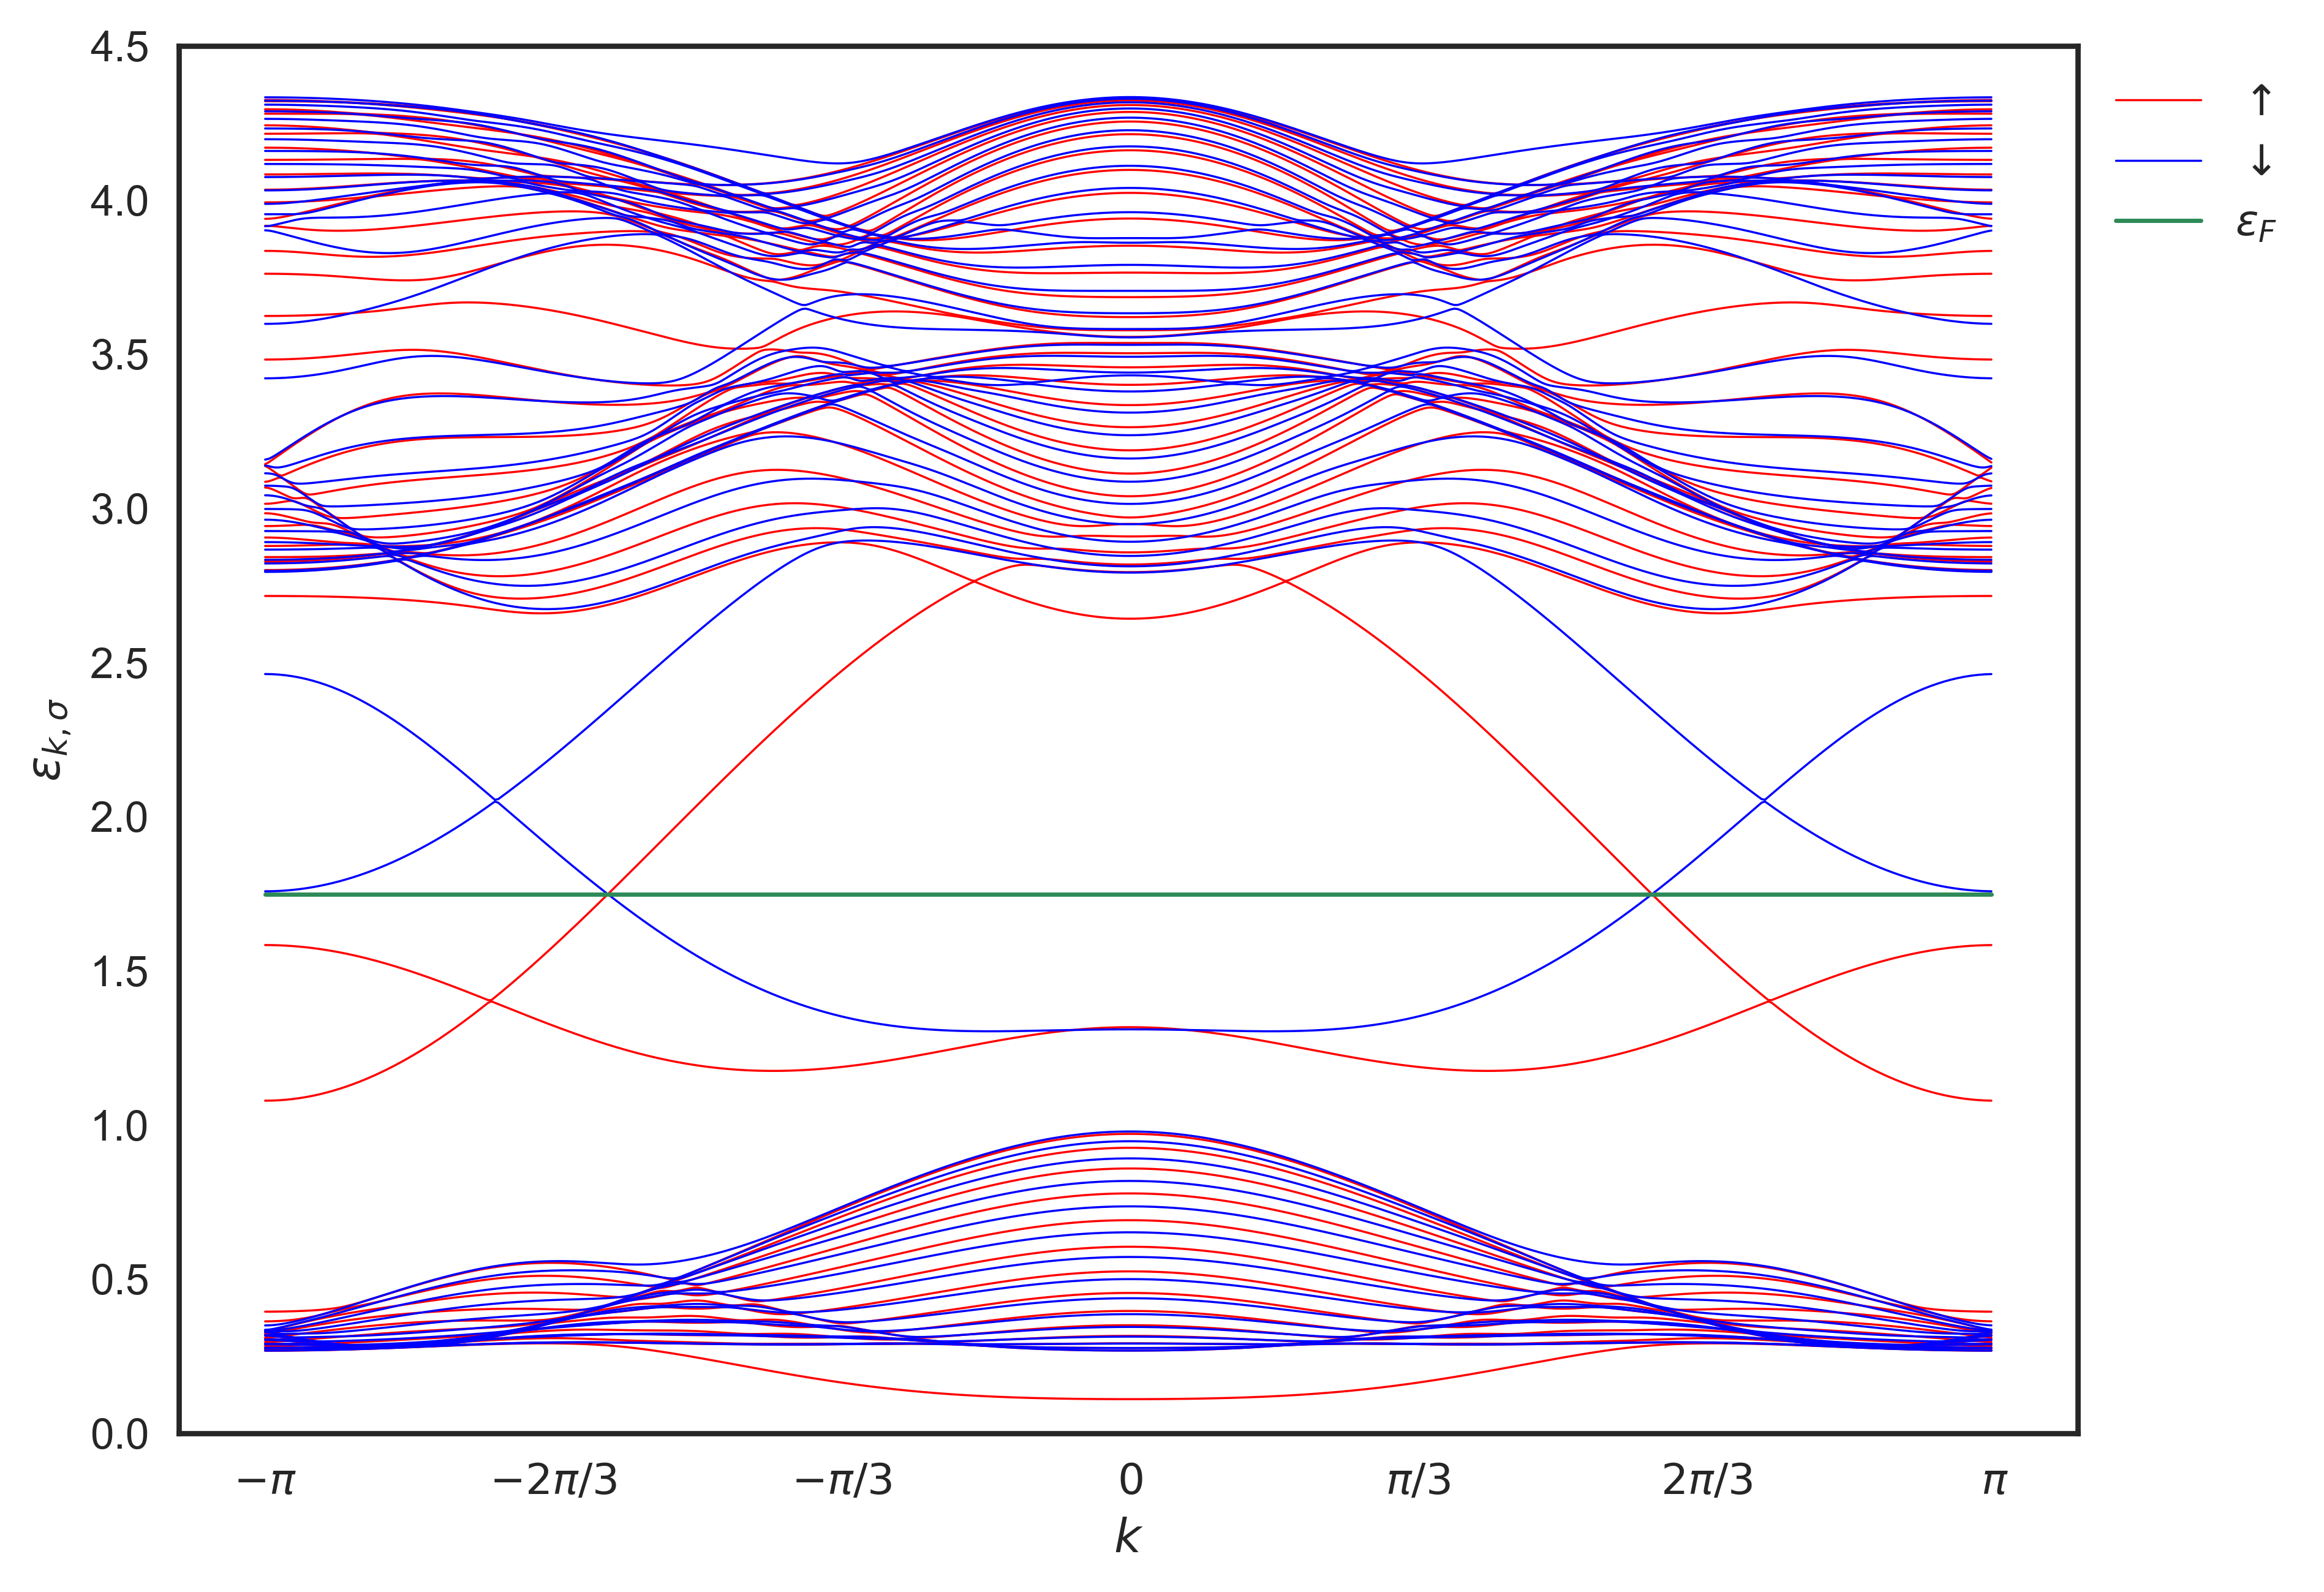
\includegraphics[scale=0.35]{Applications/tmd-mf/bands154.png}
	\caption[]{}
	\label{fig:wfs}
\end{figure}
\begin{figure}[H]
\hspace{1cm}
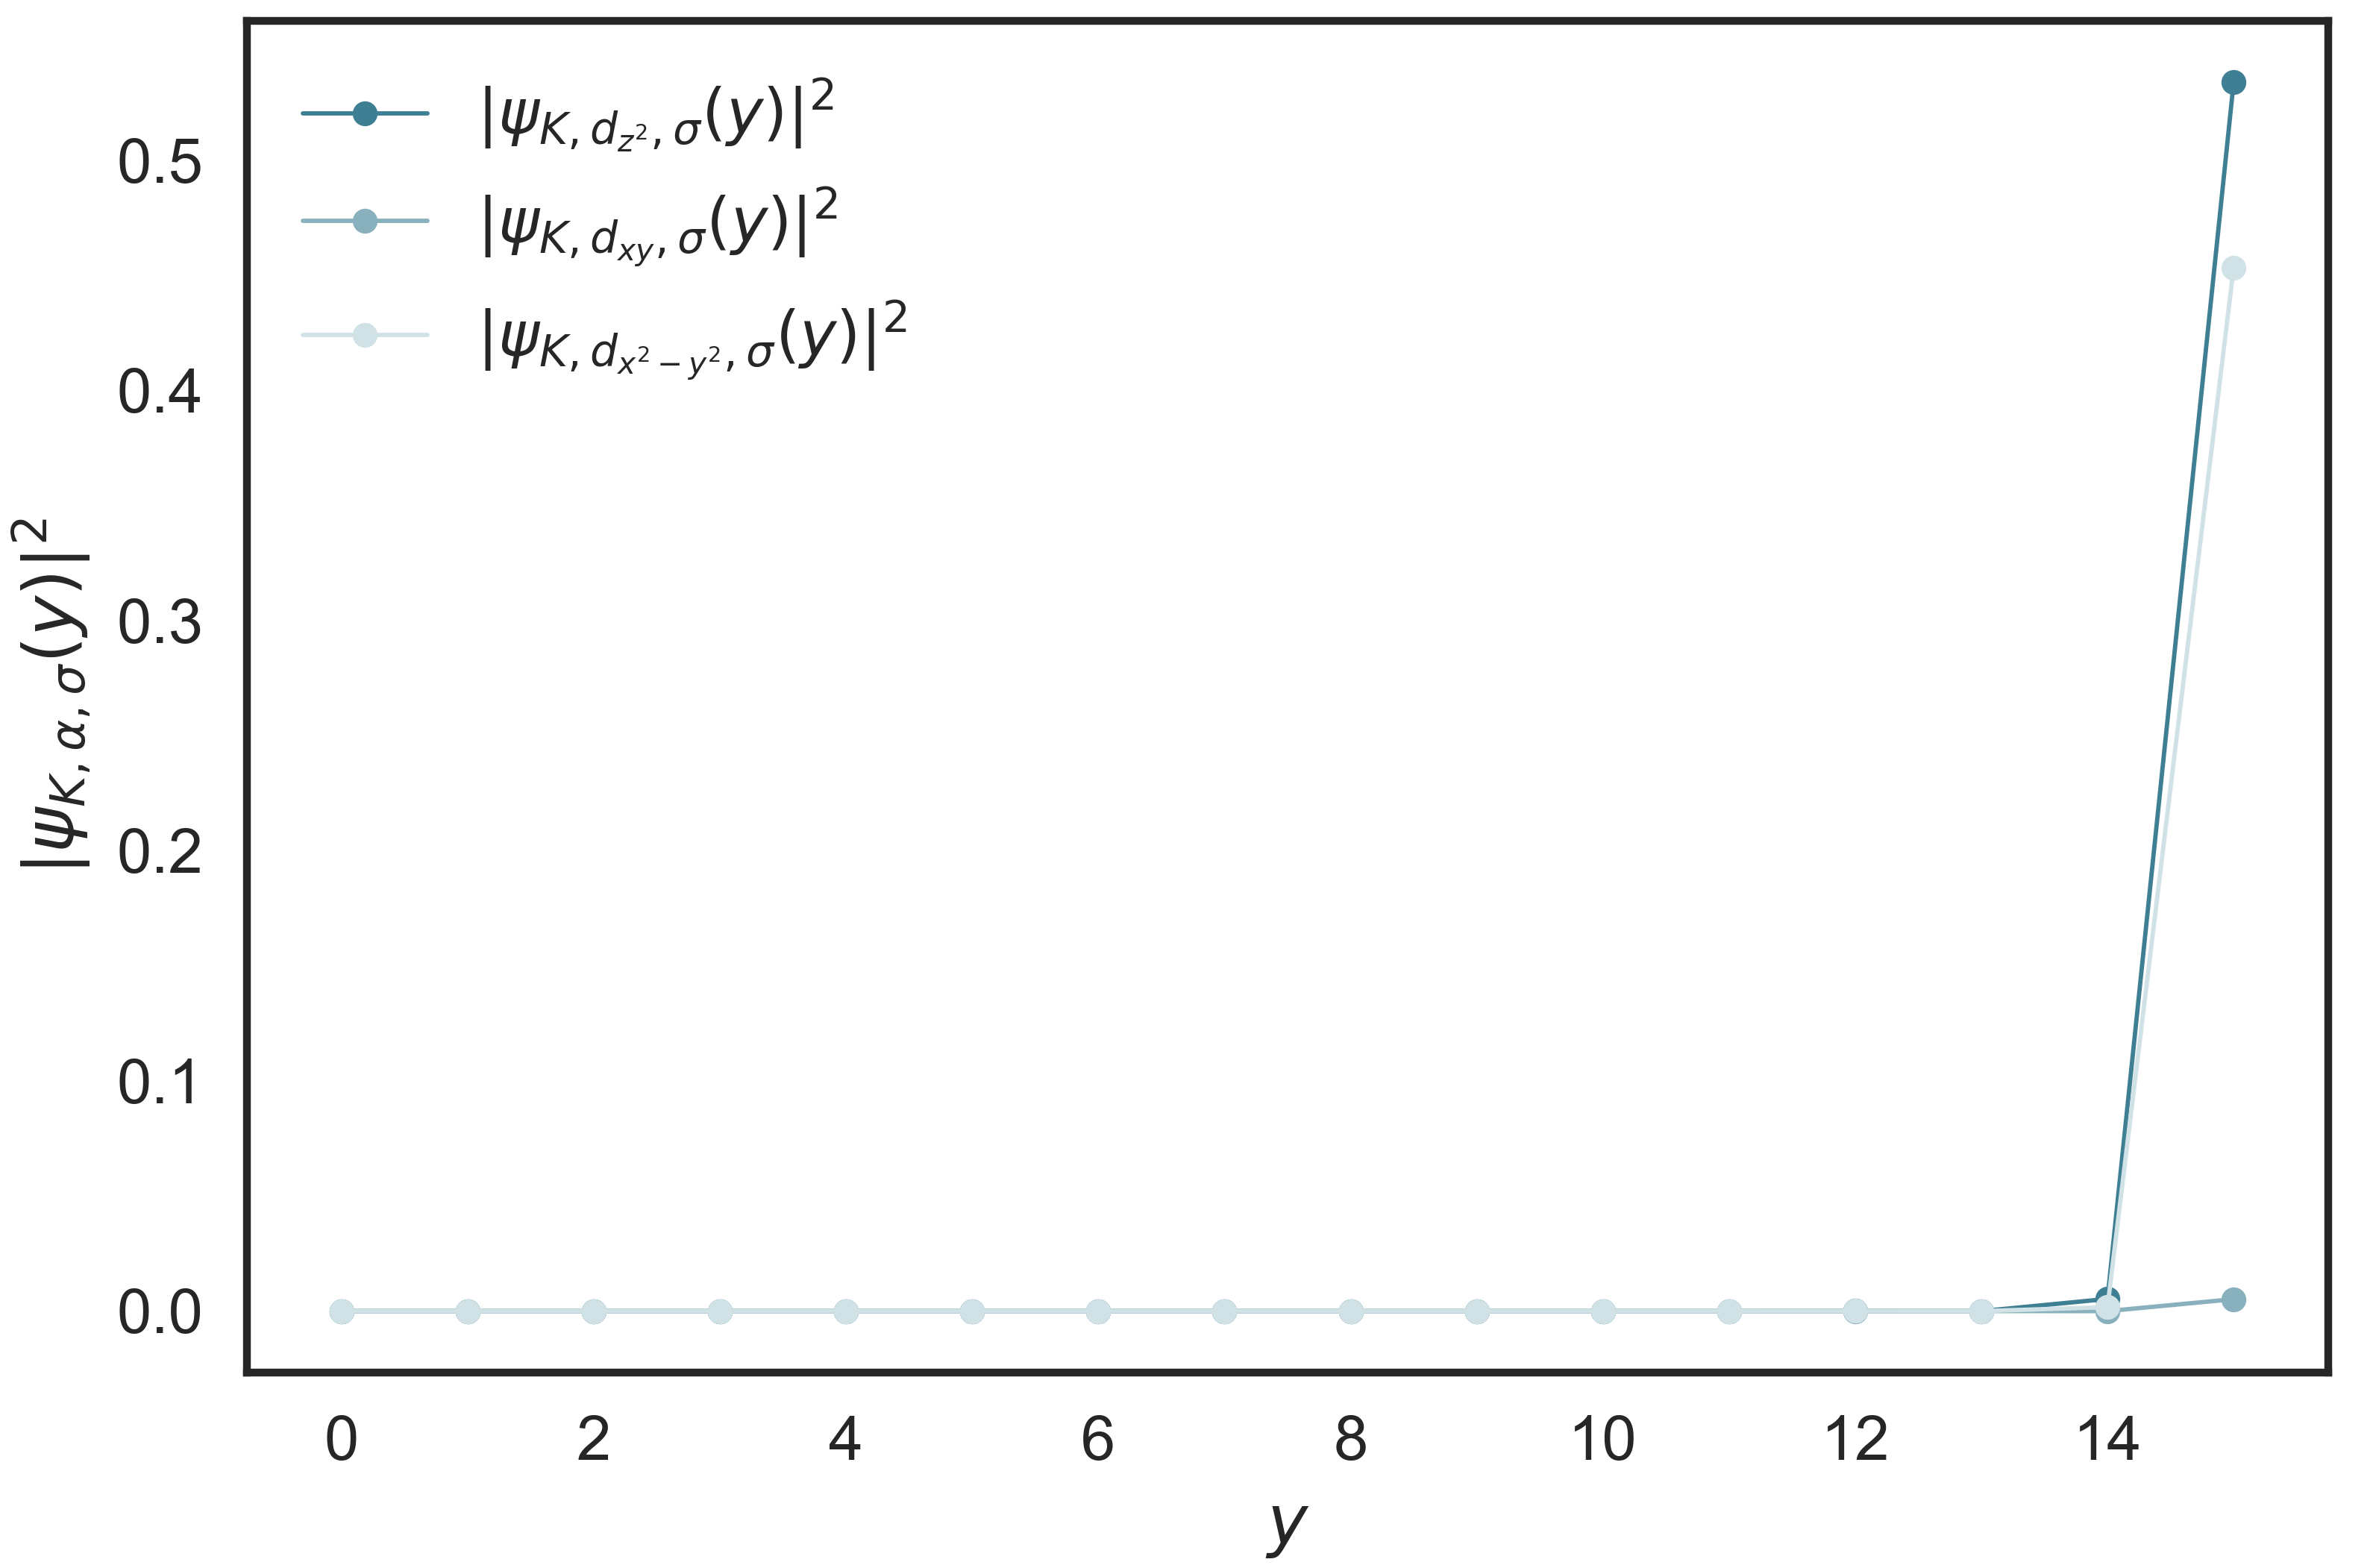
\includegraphics[scale=0.51]{Applications/tmd-mf/wfAroundK2}
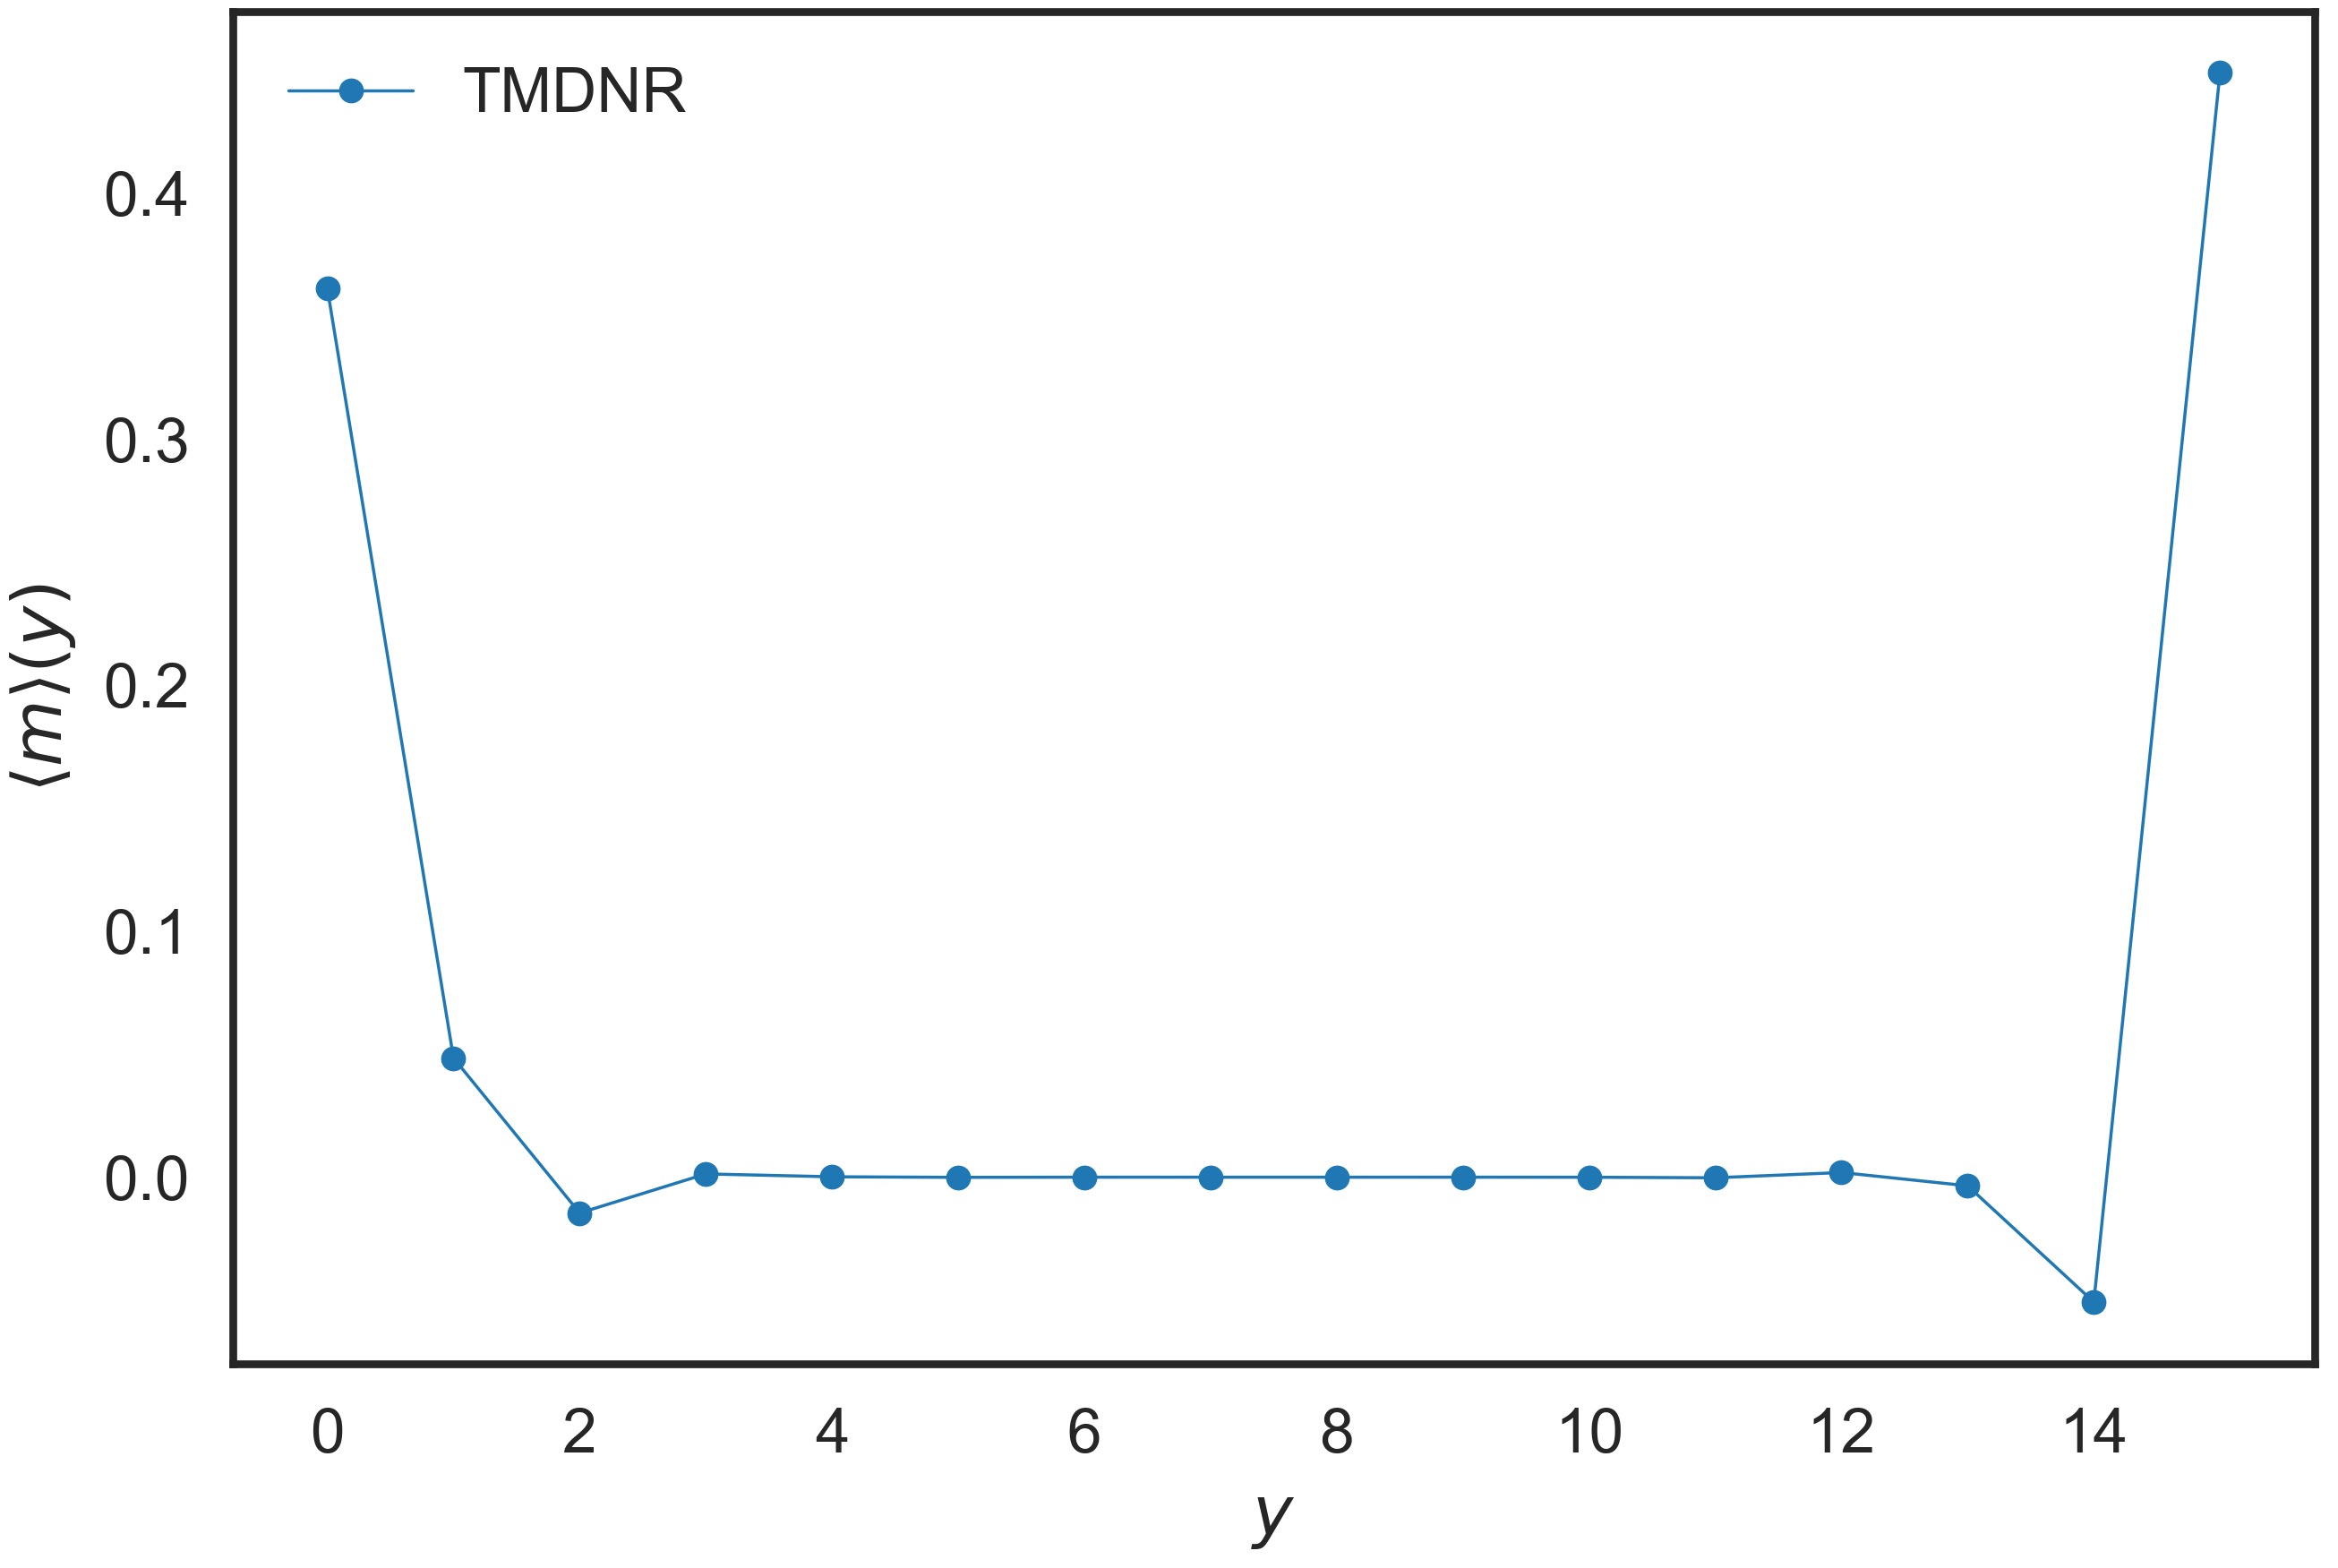
\includegraphics[scale=0.5]{Applications/tmd-mf/magProfU154}
	\caption[]{}
	\label{fig:wfs}
\end{figure}
\begin{figure}[H]
\centering
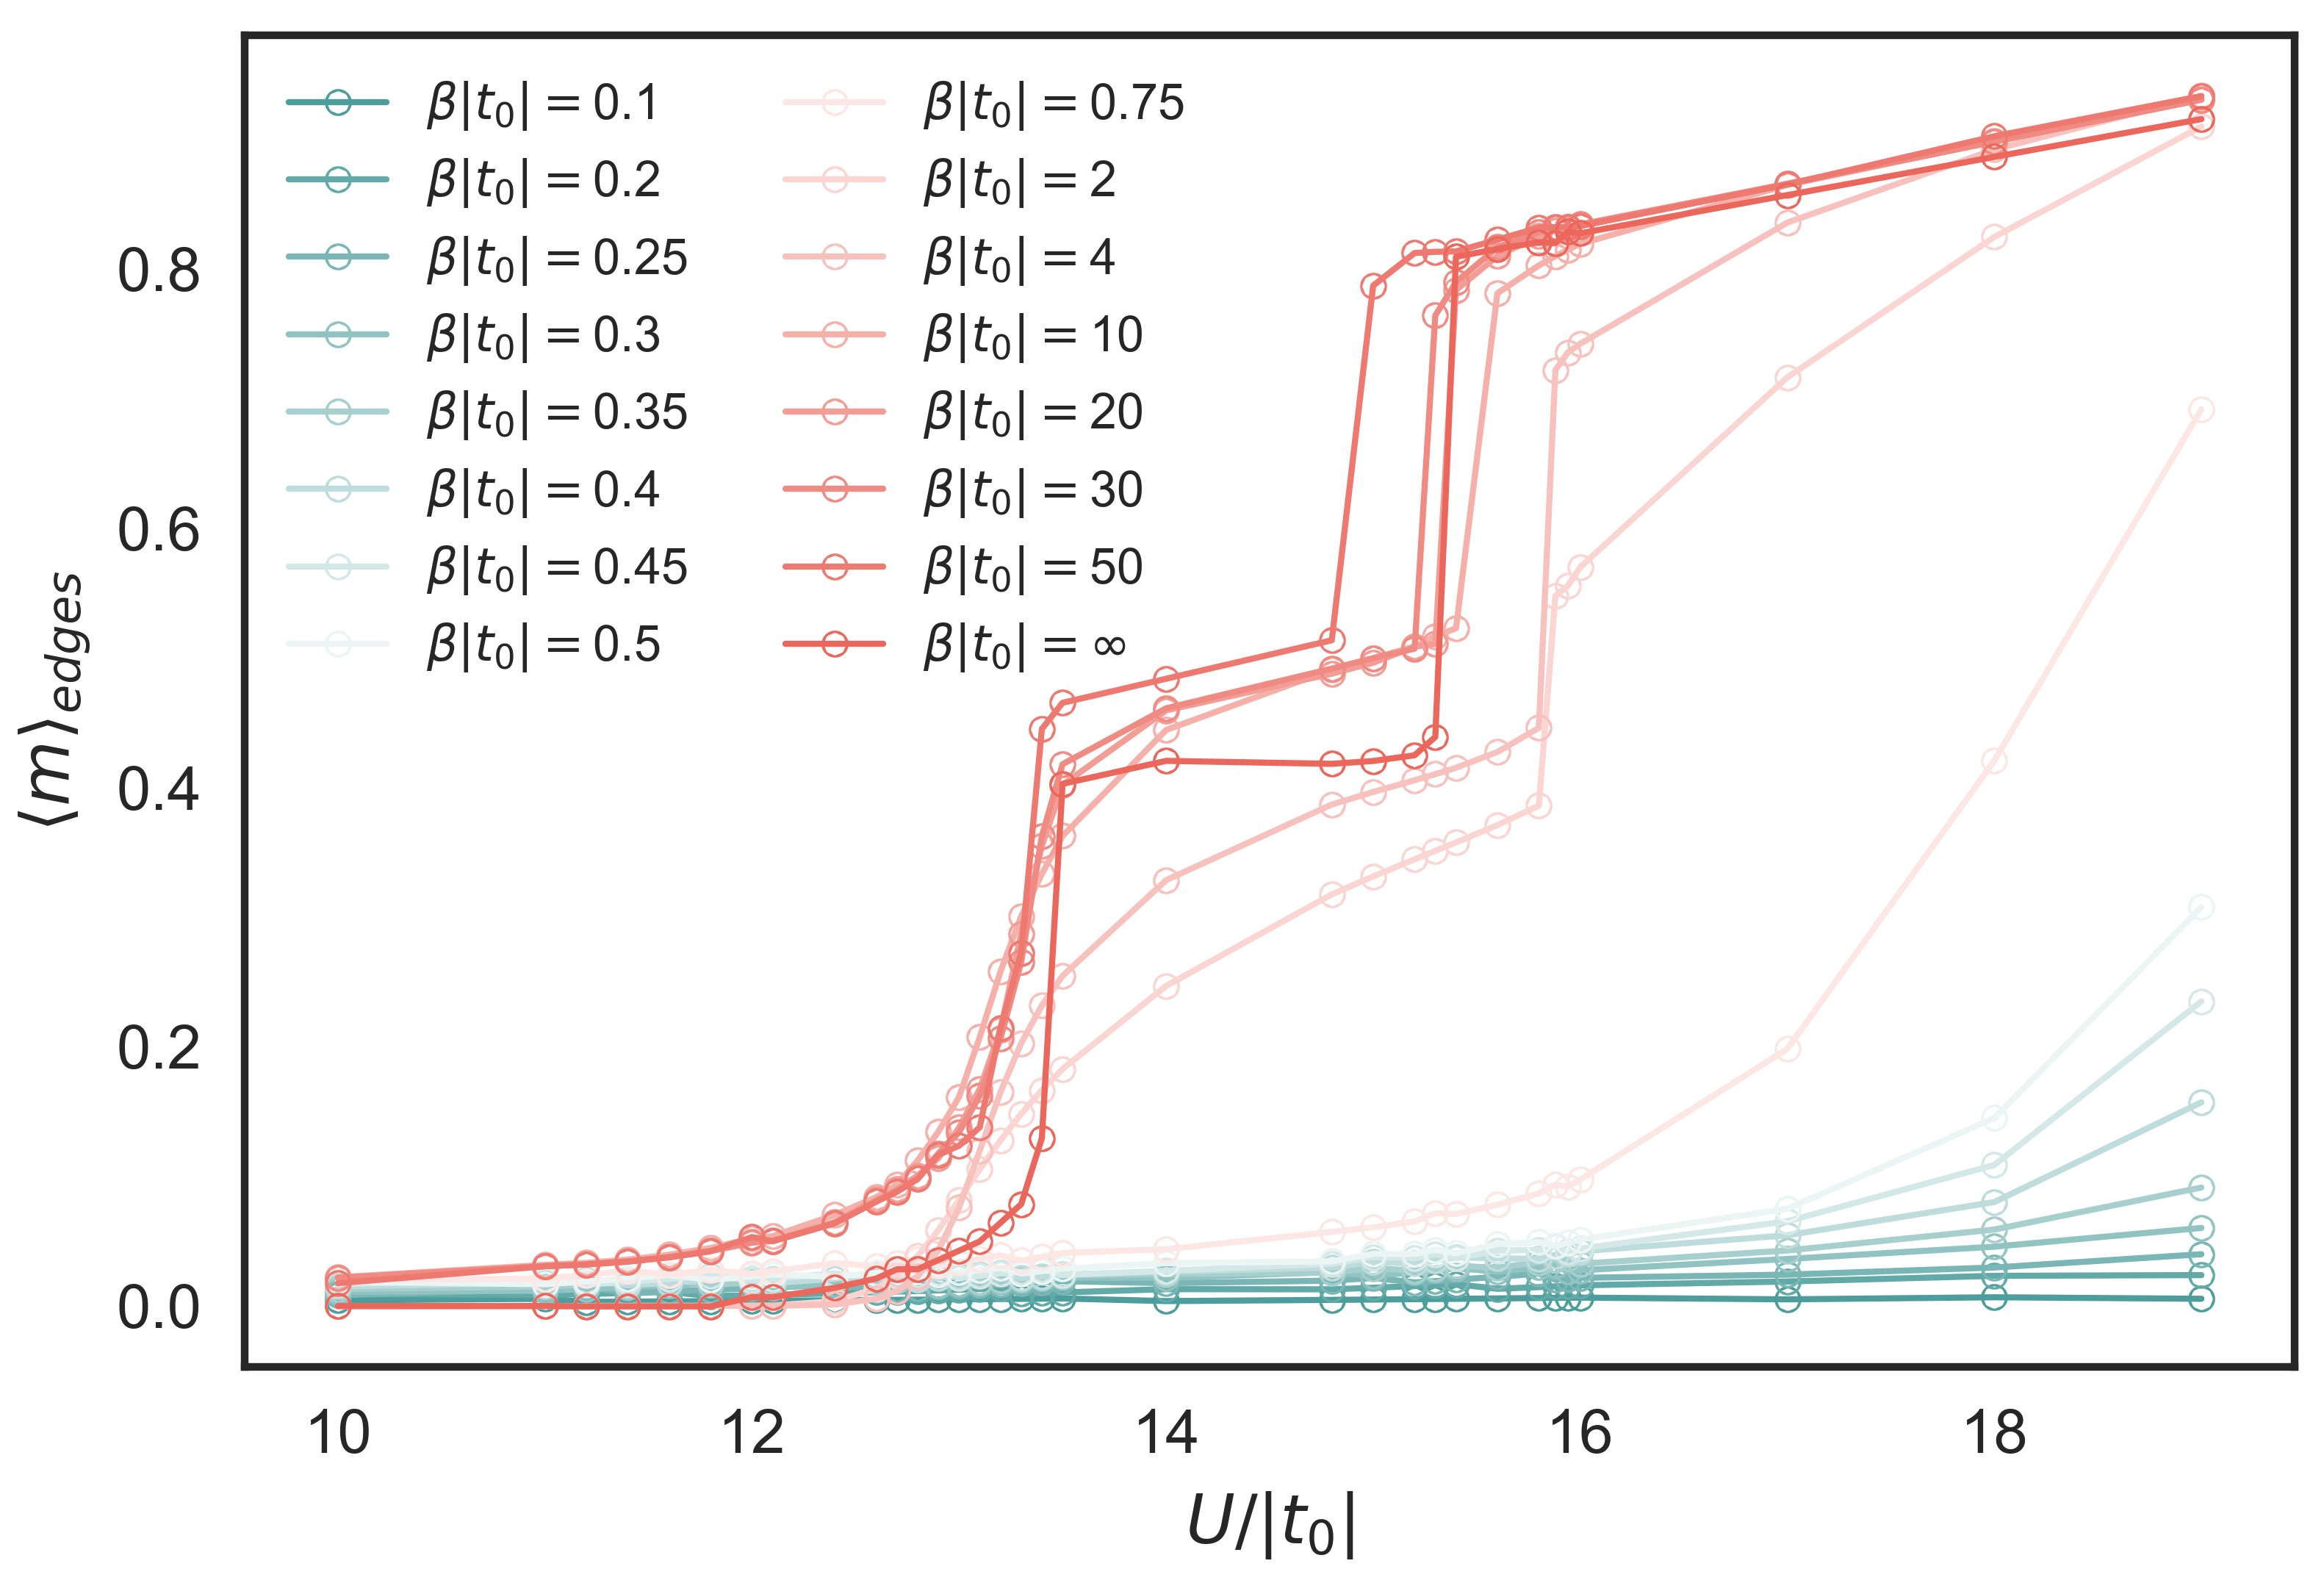
\includegraphics[scale=0.62]{Applications/tmd-mf/edge-mag-phase-diagram}
	\caption[]{}
	\label{fig:wfs}
\end{figure}
%\cleardoublepage
